%%%%%%%%%%%%%%%%%%%%%%%%%%%%%%%%%%%%%%%%%%%%%%%%%%%%%%%%%%%%%%%%%%%%%%
% Overleaf (WriteLaTeX) Example: Molecular Chemistry Presentation
%
% Source: http://www.overleaf.com
%
% In these slides we show how Overleaf can be used with standard 
% chemistry packages to easily create professional presentations.
% 
% Feel free to distribute this example, but please keep the referral
% to overleaf.com
% 
%%%%%%%%%%%%%%%%%%%%%%%%%%%%%%%%%%%%%%%%%%%%%%%%%%%%%%%%%%%%%%%%%%%%%%

\documentclass{beamer}

\mode<presentation>
{
  \usetheme{Madrid}       % or try default, Darmstadt, Warsaw, ...
  \usecolortheme{default} % or try albatross, beaver, crane, ...
  \usefonttheme{default}    % or try default, structurebold, ...
  \setbeamertemplate{navigation symbols}{}
  \setbeamertemplate{caption}[numbered]
} 

\usepackage[english]{babel}
\usepackage[utf8x]{inputenc}
\usepackage{chemfig}
\usepackage[version=3]{mhchem}

\usepackage{hyperref}
  \hypersetup{colorlinks=true}
  \hypersetup{urlcolor=blue}
  \hypersetup{linkcolor = .}
\usepackage{xcolor}
\usepackage{siunitx}
  \sisetup{separate-uncertainty = true}
\usepackage{physics}
\usepackage[font=small,labelfont=bf]{caption}
\usepackage{subcaption}
\usepackage[en-GB]{datetime2}
\usepackage{overpic}
\usepackage{feynmp}
\DeclareGraphicsRule{*}{mps}{*}{}

\usepackage{scalerel}
\newcommand{\mylbrace}[2]{\vspace{#2pt}\hspace{6pt}\scaleleftright[\dimexpr5pt+#1\dimexpr0.06pt]{\lbrace}{\rule[\dimexpr2pt-#1\dimexpr0.5pt]{-4pt}{#1pt}}{.}}
\newcommand{\myrbrace}[2]{\vspace{#2pt}\scaleleftright[\dimexpr5pt+#1\dimexpr0.06pt]{.}{\rule[\dimexpr2pt-#1\dimexpr0.5pt]{-4pt}{#1pt}}{\rbrace}\hspace{6pt}}

% Here's where the presentation starts, with the info for the title slide
\title[University of Oxford]{BESIII Physics \& Software Meeting \\Measurement of the CP even fraction \texorpdfstring{$F_+$}{F+} in \texorpdfstring{$D^0\to K^+K^-\pi^+\pi^-$}{D2KKpipi}}
\author[Martin Tat]{\textbf{Martin Tat} \hspace{0.54em} Guy Wilkinson \hspace{0.54em} Sneha Malde \hspace{0.54em} Yu Zhang}
%\author{Martin Tat}
\institute{University of Oxford}
\date{10th June 2022}

\titlegraphic{
\includegraphics[width = 2.0cm, height = 2.0cm]{OxfordLogo.pdf}\hspace{1cm}~%
              
\includegraphics[width = 3.2cm, height = 2.0cm]{bes3.jpg}}

\begin{document}

\begin{frame}
  \titlepage
\end{frame}

% These three lines create an automatically generated table of contents.
\begin{frame}{Outline}
  \tableofcontents
\end{frame}

\section{Introduction and motivation}

\begin{frame}{Introduction}
  \begin{itemize}
    \setlength\itemsep{1.5em}
    \item{Perform strong-phase analysis of $D^0\to K^+K^-\pi^+\pi^-$}
    \item{This analysis: Phase space integrated analysis}
    \begin{itemize}
      \item{$\SI{2.93}{\per\femto\barn}$ $\psi(3770)$ data from 2010-2011}
      \item{Measure CP even fraction $F_+$}
    \end{itemize}
    \item{Future analysis: Binned phase space analysis}
    \begin{itemize}
      \item{Expect $\approx\SI{20}{\per\femto\barn}$ $\psi(3770)$ data from 2010-2011 and 2021-2023}
      \item{Measure amplitude-averaged cosine and sine of strong-phase $c_i$ and $s_i$}
      \item{Plan to analyse 2021-2022 data initially}
    \end{itemize}
  \end{itemize}
\end{frame}

\begin{frame}{Introduction to GGSZ analysis of $\gamma$}
  \begin{itemize}
    \setlength\itemsep{0.5em}
    \item{Main motivation: Measure $\gamma$ in $B^\pm\to DK^\pm$ with self-conjugate multi-body $D$ decay}
    \begin{itemize}
      \item{Model independent measurement: Bins of $D$ decay phase space}
      \item{External inputs: Measure $c_i$ and $s_i$ at BESIII}
      \item{Poor binning reduces statistical sensitivity $\to$ No bias!}
    \end{itemize}
    \item{J. High Energ. Phys. 2021, 169 (2021): $B^\pm\to Dh^\pm$, $D\to K_S^0 h^+h^-$}
    \begin{itemize}
      \item{Single most precise measurement: $\gamma = (68.7^{+5.2}_{-5.1})^\circ$}
    \end{itemize}
  \end{itemize}
  \begin{figure}
    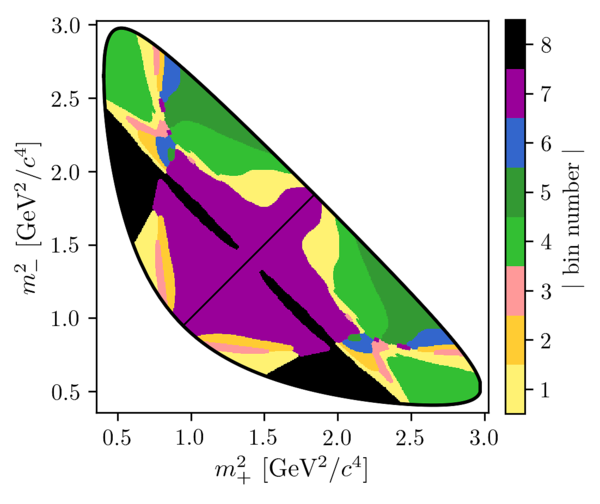
\includegraphics[height = 4cm]{Plots/KsPiPi_optimal.png}
    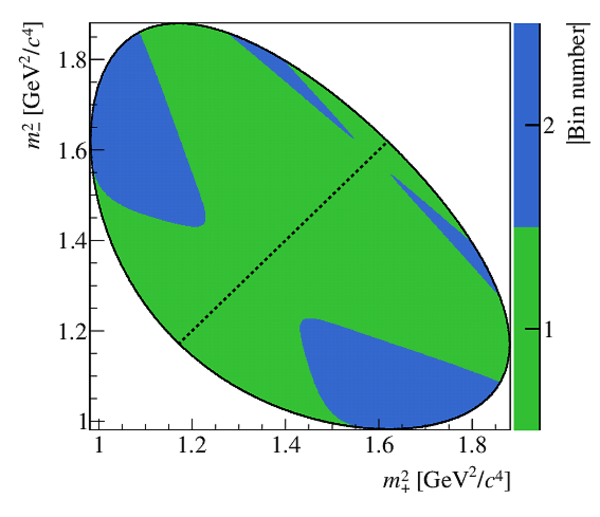
\includegraphics[height = 4cm]{Plots/KsKK_binning.png}
  \end{figure}
\end{frame}

\begin{frame}{Introduction to GGSZ analysis of $\gamma$}
  \begin{itemize}
    \setlength\itemsep{0.5em}
    \item{Our aim: Analyse $B^\pm\to[K^+K^-\pi^+\pi^-]_D h^\pm$ in bins of phase space}
    \begin{itemize}
    \setlength\itemsep{0.5em}
      \item{Develop binning scheme using LHCb model \href{https://arxiv.org/abs/1811.08304}{JHEP 02 (2019) 126}}
      \item{Simultaneously analyse $c_i$/$s_i$ at BESIII and $\gamma$ at LHCb}
      \item{Expected precision $\Delta\gamma\approx 12^\circ$ with LHCb Run\,1+2}
    \end{itemize}
  \end{itemize}
  \begin{figure}
    \centering
    \begin{subfigure}{0.5\textwidth}
      \centering
      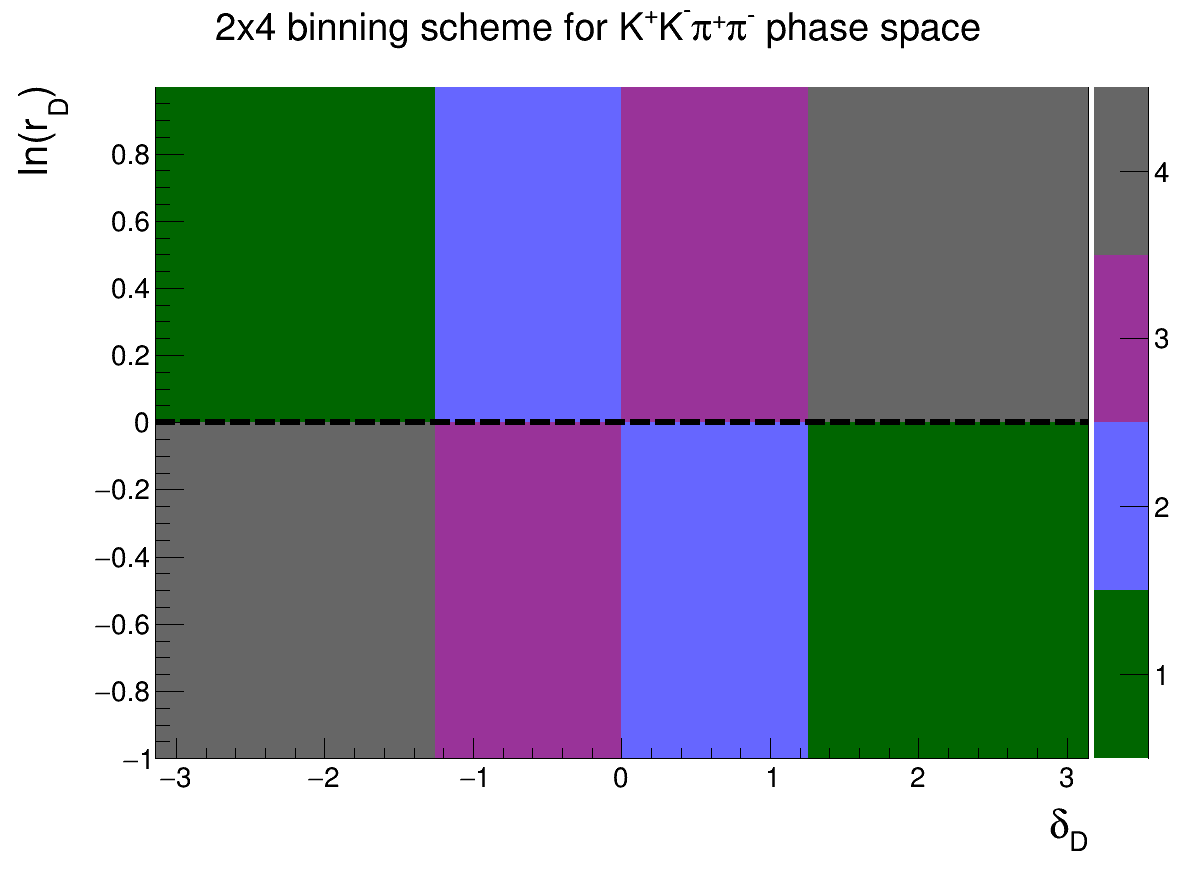
\includegraphics[width=1.0\textwidth]{Plots/BinningSchemePlot_4Bins.png}
      \caption{$2\times 4$ bins}
    \end{subfigure}%
    \begin{subfigure}{0.5\textwidth}
      \centering
      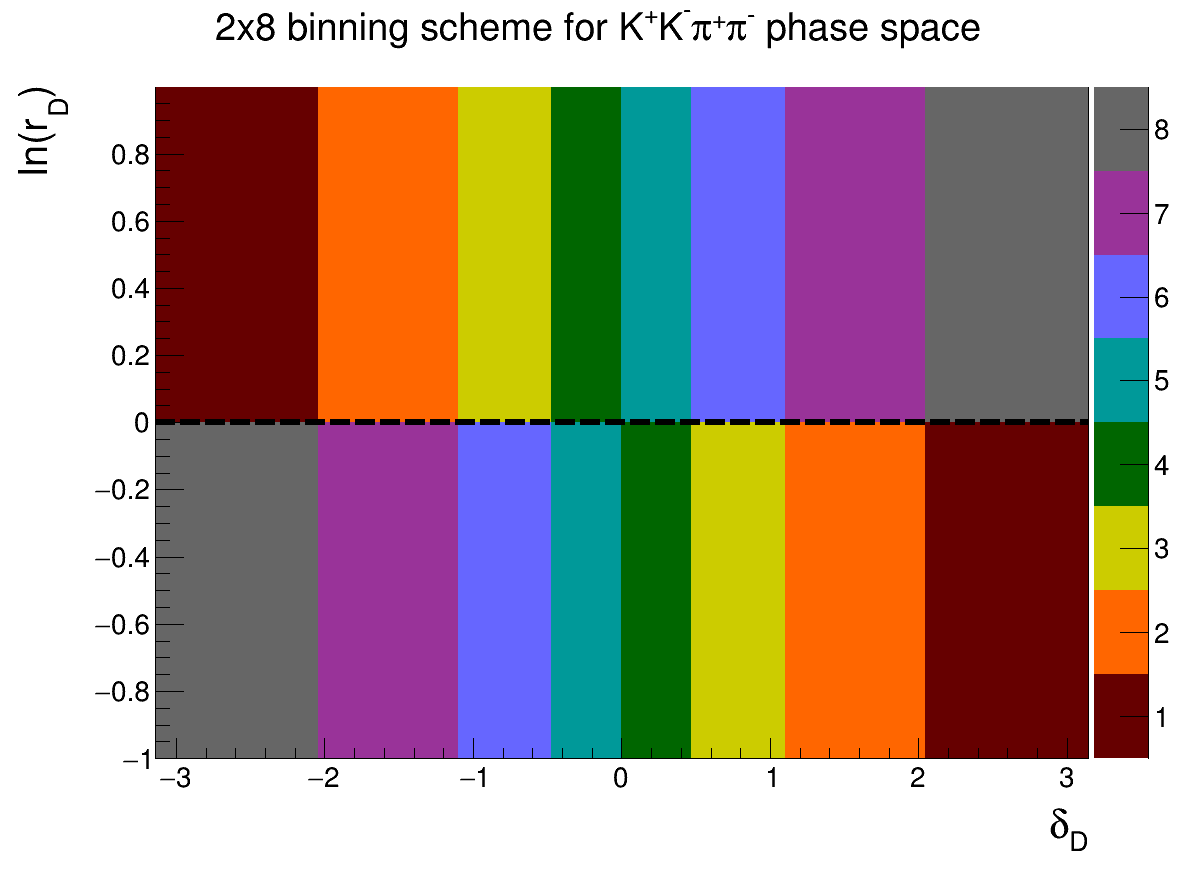
\includegraphics[width=1.0\textwidth]{Plots/BinningSchemePlot_8Bins.png}
      \caption{$2\times 8$ bins}
    \end{subfigure}
    \caption{Binning scheme for $D^0\to K^+K^-\pi^+\pi^-$}
  \end{figure}
\end{frame}

\begin{frame}{Introduction to $D$ mixing and CP-violation}
  \begin{itemize}
    \setlength\itemsep{0.0em}
    \item{$D\to KK\pi\pi$ can also be used to study $D$-mixing}
    \item{Phase space integrated analysis:}
    \begin{itemize}
      \item{\href{https://arxiv.org/abs/1502.04560}{Physical Review D, 91(9), 2015}}
      \item{Measure mixing parameter $y_{\rm CP}$ and CP-violation parameter $A_\Gamma$ in self-conjugate multi-body decays}
    \end{itemize}
    \item{Analysis in bins of phase space:}
    \begin{itemize}
      \item{\href{https://arxiv.org/abs/2106.03744}{Phys. Rev. Lett. 127, 111801 (2021)}}
      \item{Bin-flip analysis of $D\to K_S\pi\pi$}
      \item{Measure mixing parameters $x$, $y$ and CP-violation parameters $|q/p|$, $\varphi$}
    \end{itemize}
  \end{itemize}
  \begin{figure}
    \centering
    \begin{subfigure}{0.4\textwidth}
      \centering
      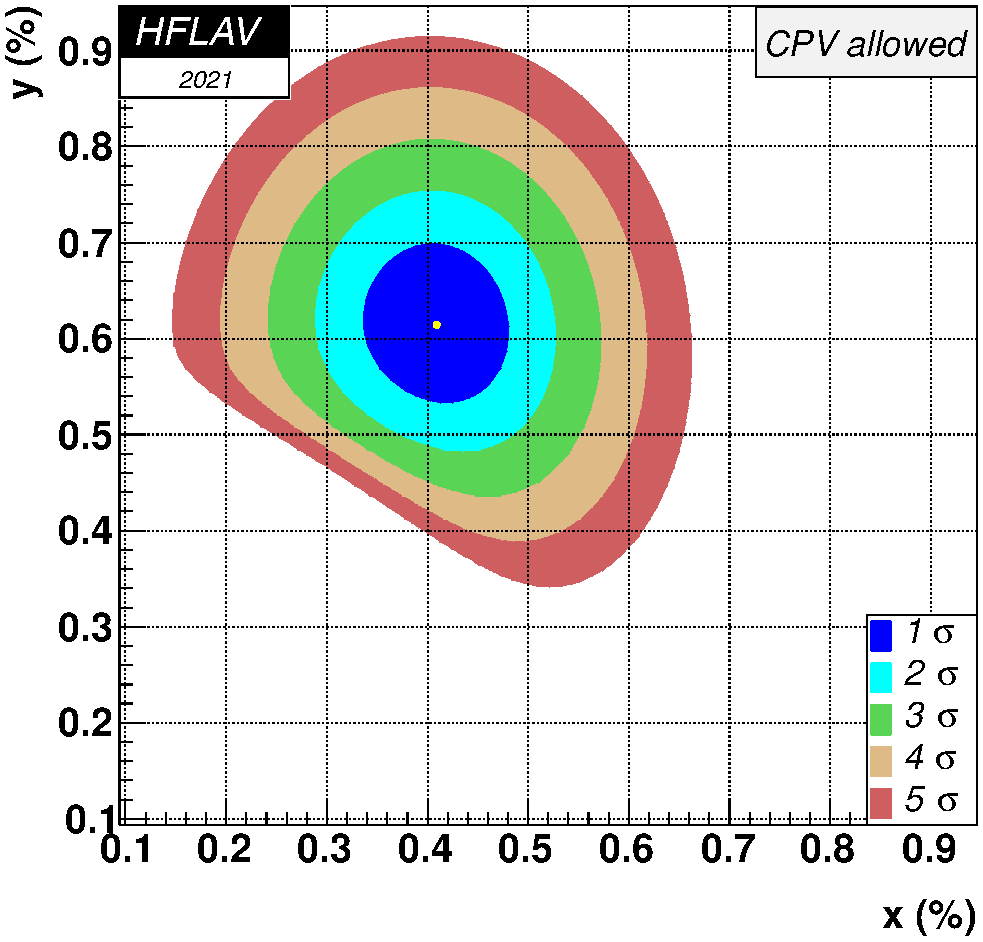
\includegraphics[width=0.6\textwidth]{Plots/fig_plot_xy2d.pdf}
      \caption{Source: \href{https://hflav-eos.web.cern.ch/hflav-eos/charm/CKM21/results_mix_cpv.html}{HFLAV}}
    \end{subfigure}%
    \begin{subfigure}{0.4\textwidth}
      \centering
      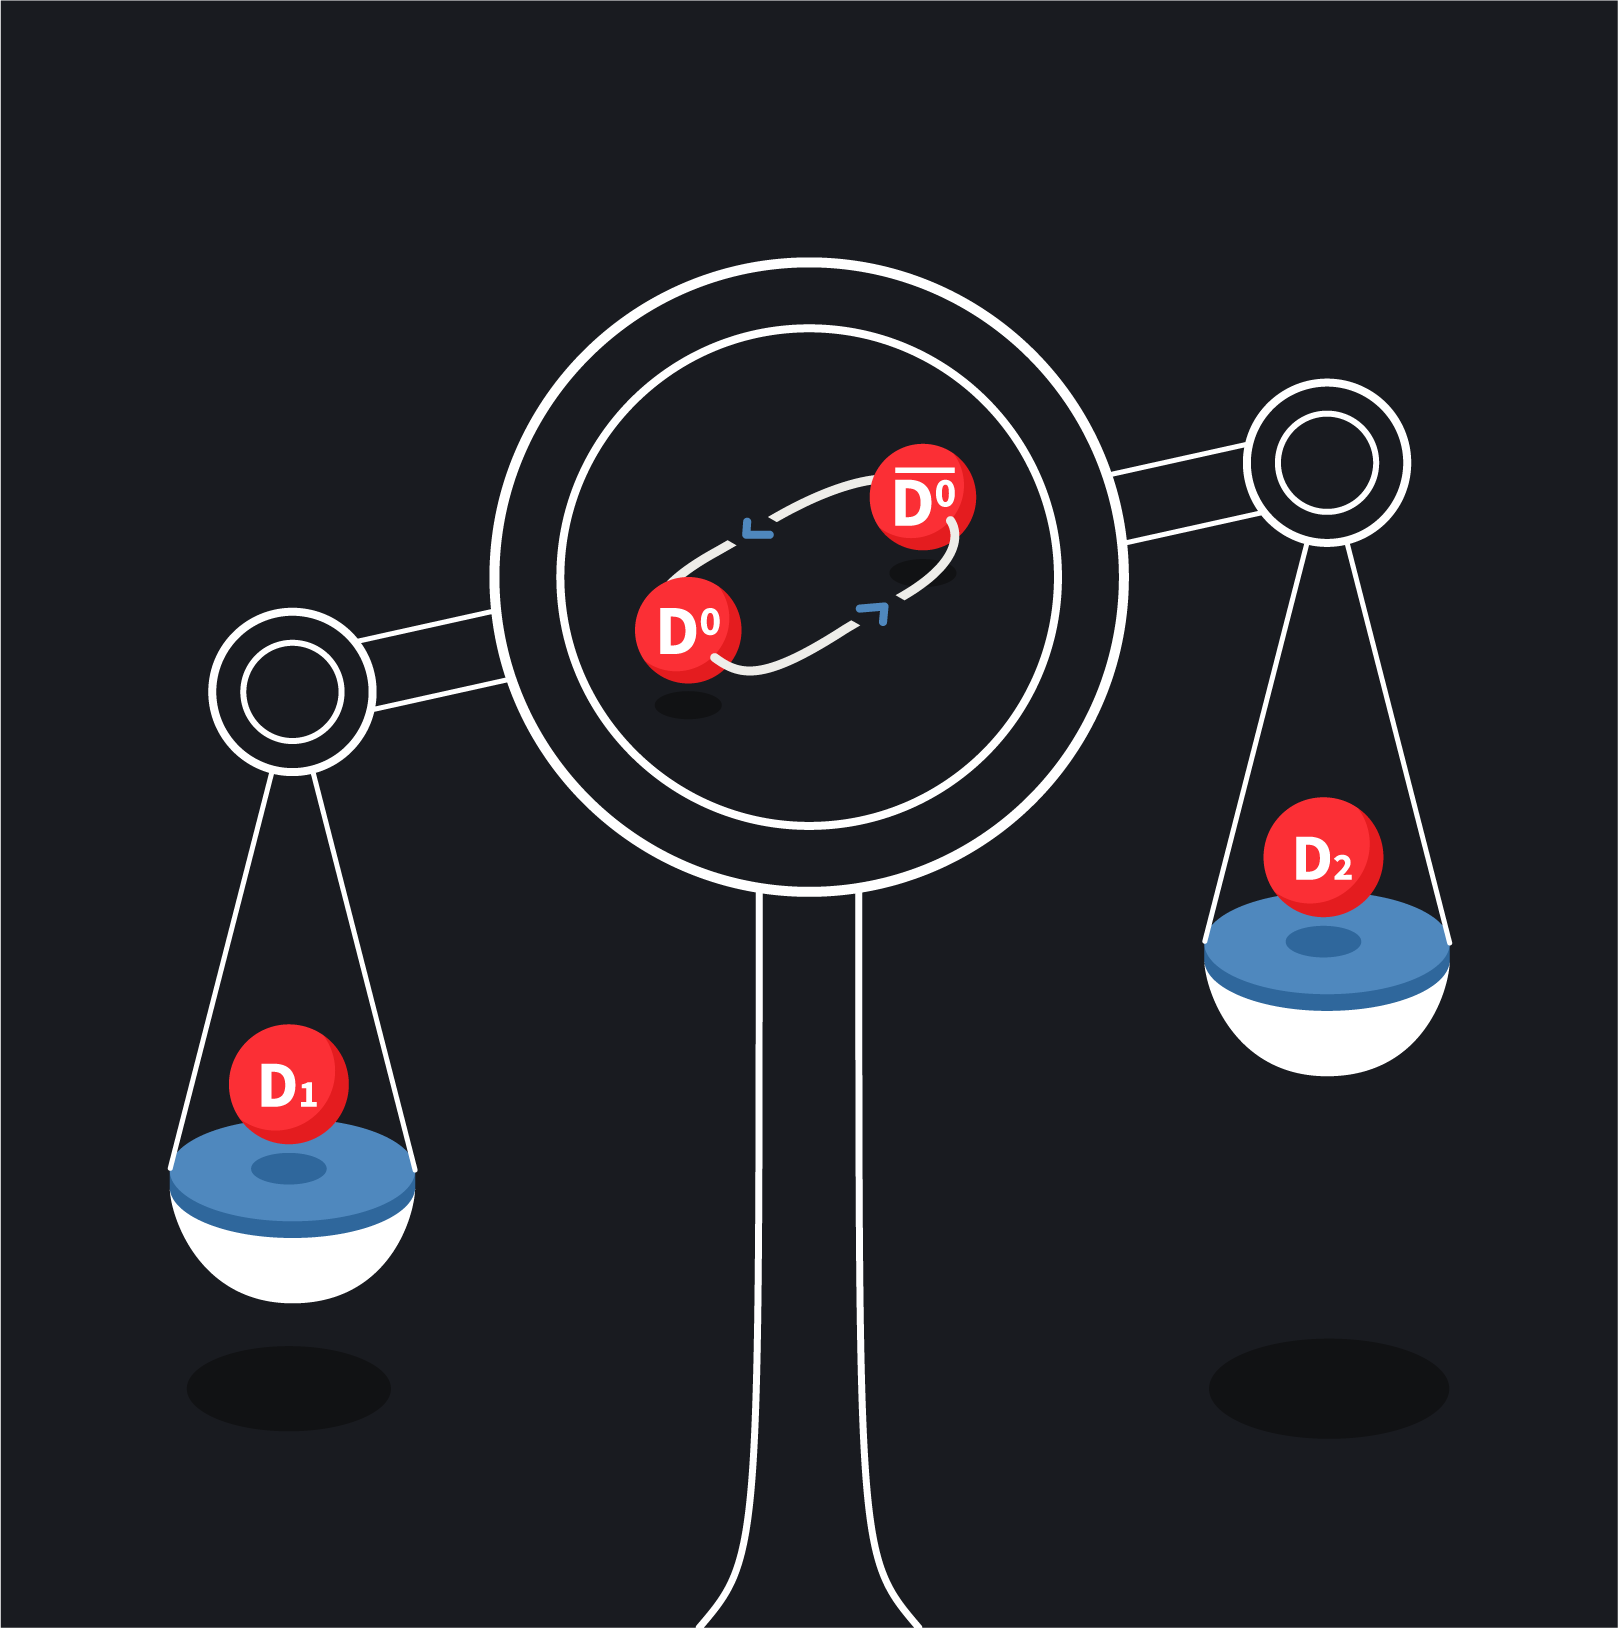
\includegraphics[width=0.55\textwidth]{Plots/D0OscArt.png}
      \caption{Source: \href{https://lhcb-outreach.web.cern.ch/2021/06/08/first-observation-of-the-mass-difference-between-neutral-charm-mesons/}{LHCb outreach}}
    \end{subfigure}
  \end{figure}
\end{frame}


\begin{frame}{Motivation for $F_+$ measurement}
  \begin{itemize}
    \setlength\itemsep{1.0em}
    \item{$F_+$ describes the CP content of a self-conjugate multi-body decay}
    \begin{itemize}
      \item{$F_+ = 1$ ($0$) for CP even (odd) final states}
    \end{itemize}
    \item{$F_+$ can be measured with current $\SI{3}{\per\femto\barn}$ dataset}
    \begin{itemize}
      \item{First model independent measurement of $F_+^{KK\pi\pi}$!}
      \item{Useful to test agreement with LHCb model prediction: $F_+ = 0.736$}
    \end{itemize}
    \item{Important input to quasi-GLW analysis of the CKM angle $\gamma$}
    \begin{itemize}
      \item{Current GLW modes: $KK$, $\pi\pi$, $\pi\pi\pi\pi$}
      \item{Minimal effort to include $KK\pi\pi$ in GLW analyses $\implies$ More statistics}
    \end{itemize}
    \item{Other $F_+$ measurements:}
    \begin{itemize}
      \item{$D^0\to\pi^+\pi^-\pi^+\pi^-$ \href{https://arxiv.org/abs/1709.03467}{JHEP 01 (2018) 144}}
      \item{$D^0\to K_S\pi^+\pi^-\pi^0$ \href{https://arxiv.org/abs/1710.10086}{JHEP 01 (2018) 82}}
      \item{$D^0\to h^+h^-\pi^0$ \href{https://arxiv.org/abs/1504.05878}{Physics Letters B 747 (2015)}}
      \item{Measurements are from CLEO-c, BESIII analyses ongoing}
    \end{itemize}
  \end{itemize}
\end{frame}

\section{Strategy of strong-phase analysis}
\begin{frame}{Strategy for strong-phase analysis}
  \begin{enumerate}
    \setlength\itemsep{0.5em}
    \item{Select double tags of $KK\pi\pi$ vs flavour, CP and self-conjugate tags}
    \item{Normalise double tag yields by the corresponding single tag yields}
    \item{Measure flavour tag yields $K_i$}
    \item{Fit $c_i$ with CP tags and $c_i$+$s_i$ with self-conjugate tags:}
  \end{enumerate}
  \begin{block}{$c_i$/$s_i$ analysis: Bins of $KK\pi\pi$ phase space}
    CP: $M_i\propto\big(K_i + K_{-i} - 2c_i\sqrt{K_iK_{-i}}(2F_+^{\rm tag} - 1)\big)$ \\
    Self-conjugate: $M_{ij}\propto\big(K_iK_{-j}^\prime + K_{-i}K_j^\prime - 2\sqrt{K_iK_{-i}K_j^\prime K_{-j}^\prime}(c_ic_j^\prime + s_is_{-j}^\prime\big)$
  \end{block}
  \begin{block}{$F_+$ analysis: Sum over all $KK\pi\pi$ phase space bins}
    CP: $M\propto\big(1 - 2(2F_+^{KK\pi\pi} - 1)(2F_+^{\rm tag} - 1)\big)$ \\
    Self-conjugate: $M_j\propto\big(K_j^\prime + K_{-j}^\prime - 2c_j^{\prime}\sqrt{K_j^\prime K_{-j}^\prime}(2F_+^{KK\pi\pi} - 1)\big)$
  \end{block}
\end{frame}

\section{Selection}
\begin{frame}{Selection}
  \begin{itemize}
    \item{Selection of charged and neutral particles follow standard track and shower requirements}
    \item{Require flight significance $> 2$ for $K_S$}
    \item{$K_S$ veto for $KK\pi\pi$ and $\pi\pi\pi^0$ tags}
    \item{$\Delta E$ cut of $3\sigma$}
    \item{$\Delta E$ fit for 4-body modes allows a non-smooth background at $\Delta E = 0$}
  \end{itemize}
  \begin{figure}
    \centering
    \begin{subfigure}{0.5\textwidth}
      \centering
      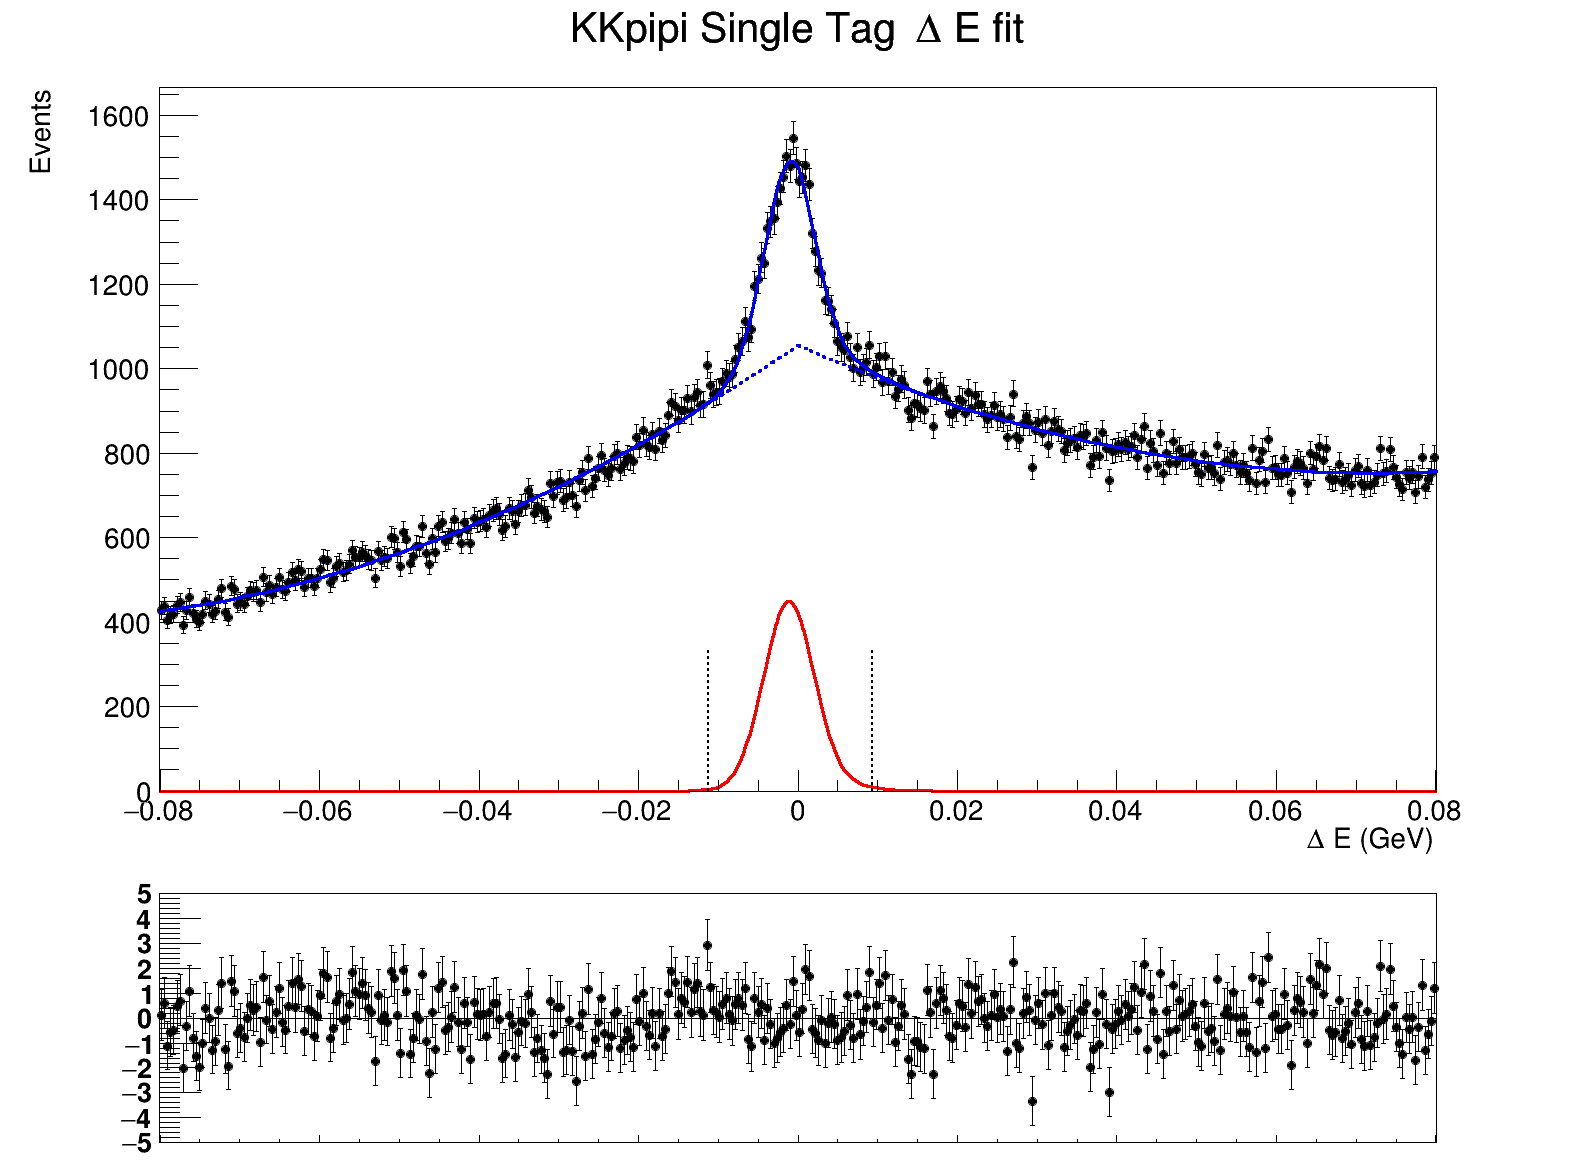
\includegraphics[width=\textwidth, clip = true, trim = {0 11cm 0 0 }]{Plots/KKpipi_SingleTag_DeltaE_Plot.png}
    \end{subfigure}%
    \begin{subfigure}{0.5\textwidth}
      \centering
      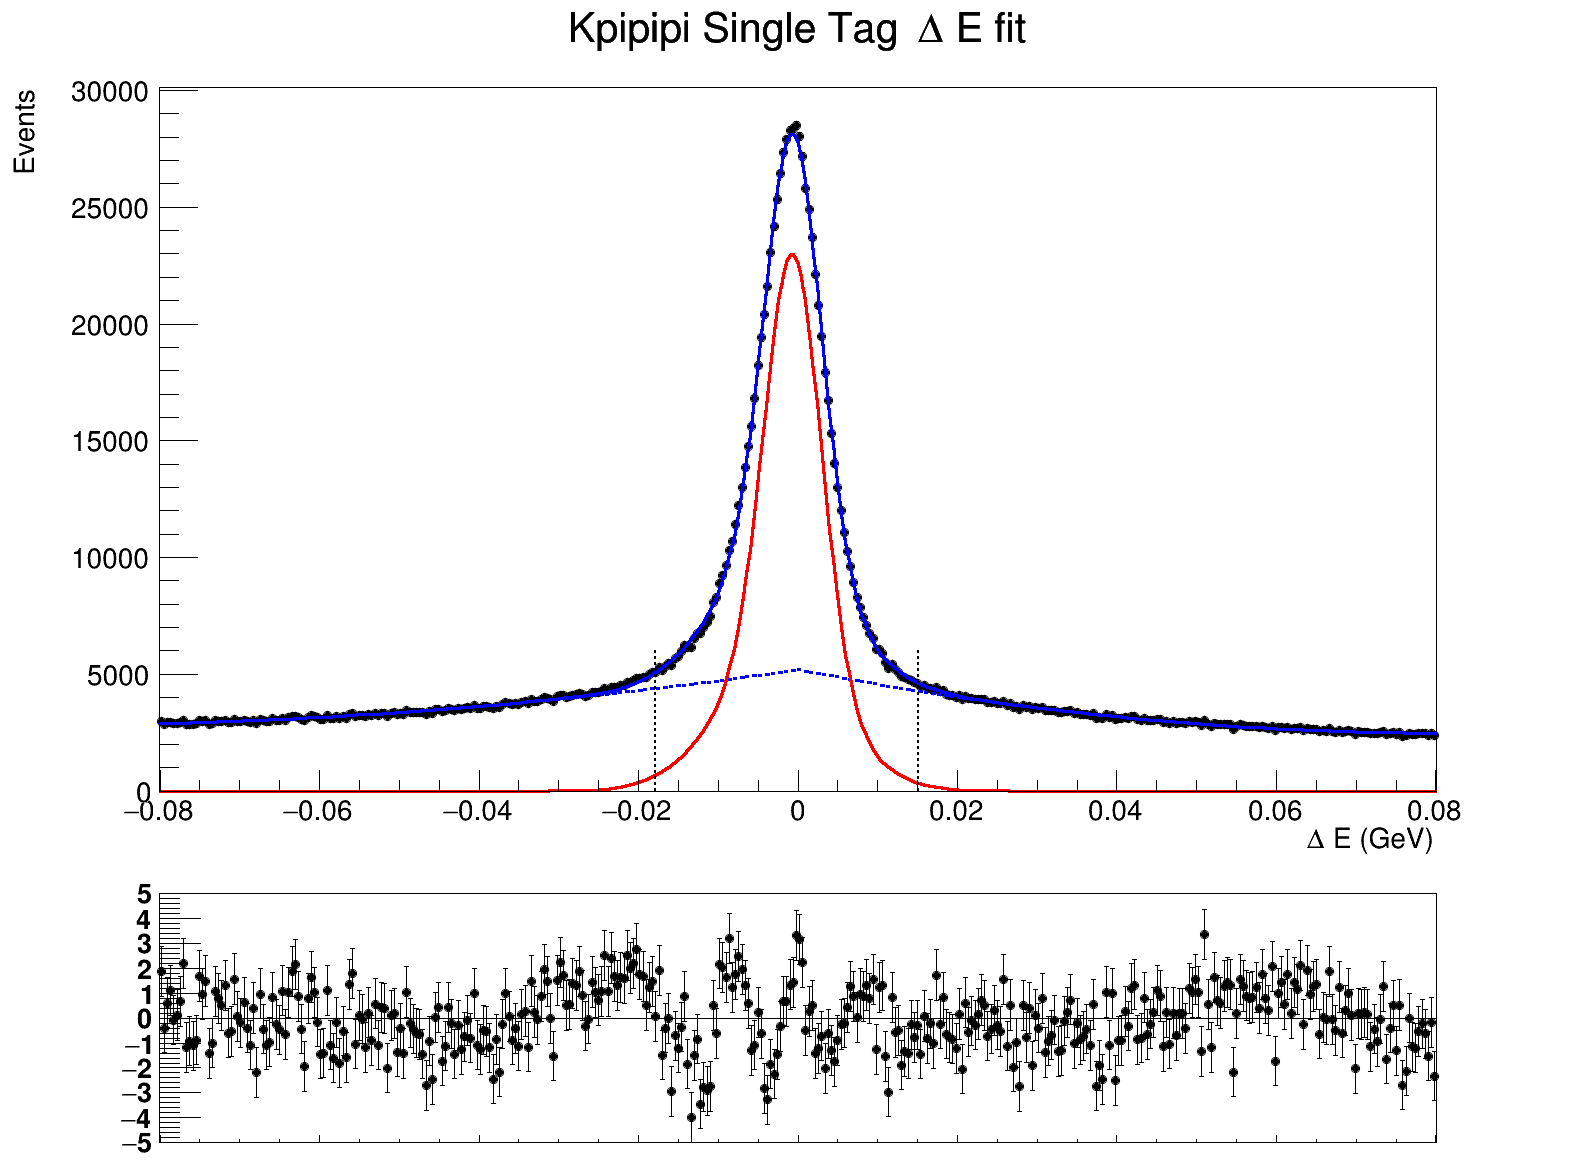
\includegraphics[width=\textwidth, clip = true, trim = {0 11cm 0 0 }]{Plots/Kpipipi_SingleTag_DeltaE_Plot.png}
    \end{subfigure}
    \caption{Double Gaussian signal and Chebychev polynomial background}
  \end{figure}
\end{frame}

\section{Fit of single tag yields}
\begin{frame}{Single tag fits}
  \begin{itemize}
    \item{Fit strategy: Fit $m_{\rm BC}$}
    \item{Fit model:}
    \begin{itemize}
      \item{Signal: PDF from signal MC, convoluted with single or double Gaussian}
      \item{Flat background: Argus PDF}
      \item{Peaking background shape and yield fixed}
      \begin{itemize}
        \item{Fit shape to dedicated MC samples}
        \item{Calculate yield from ratios of efficiencies and branching fractions}
      \end{itemize}
    \end{itemize}
  \end{itemize}
  \begin{figure}
    \centering
    \begin{subfigure}{0.5\textwidth}
      \centering
      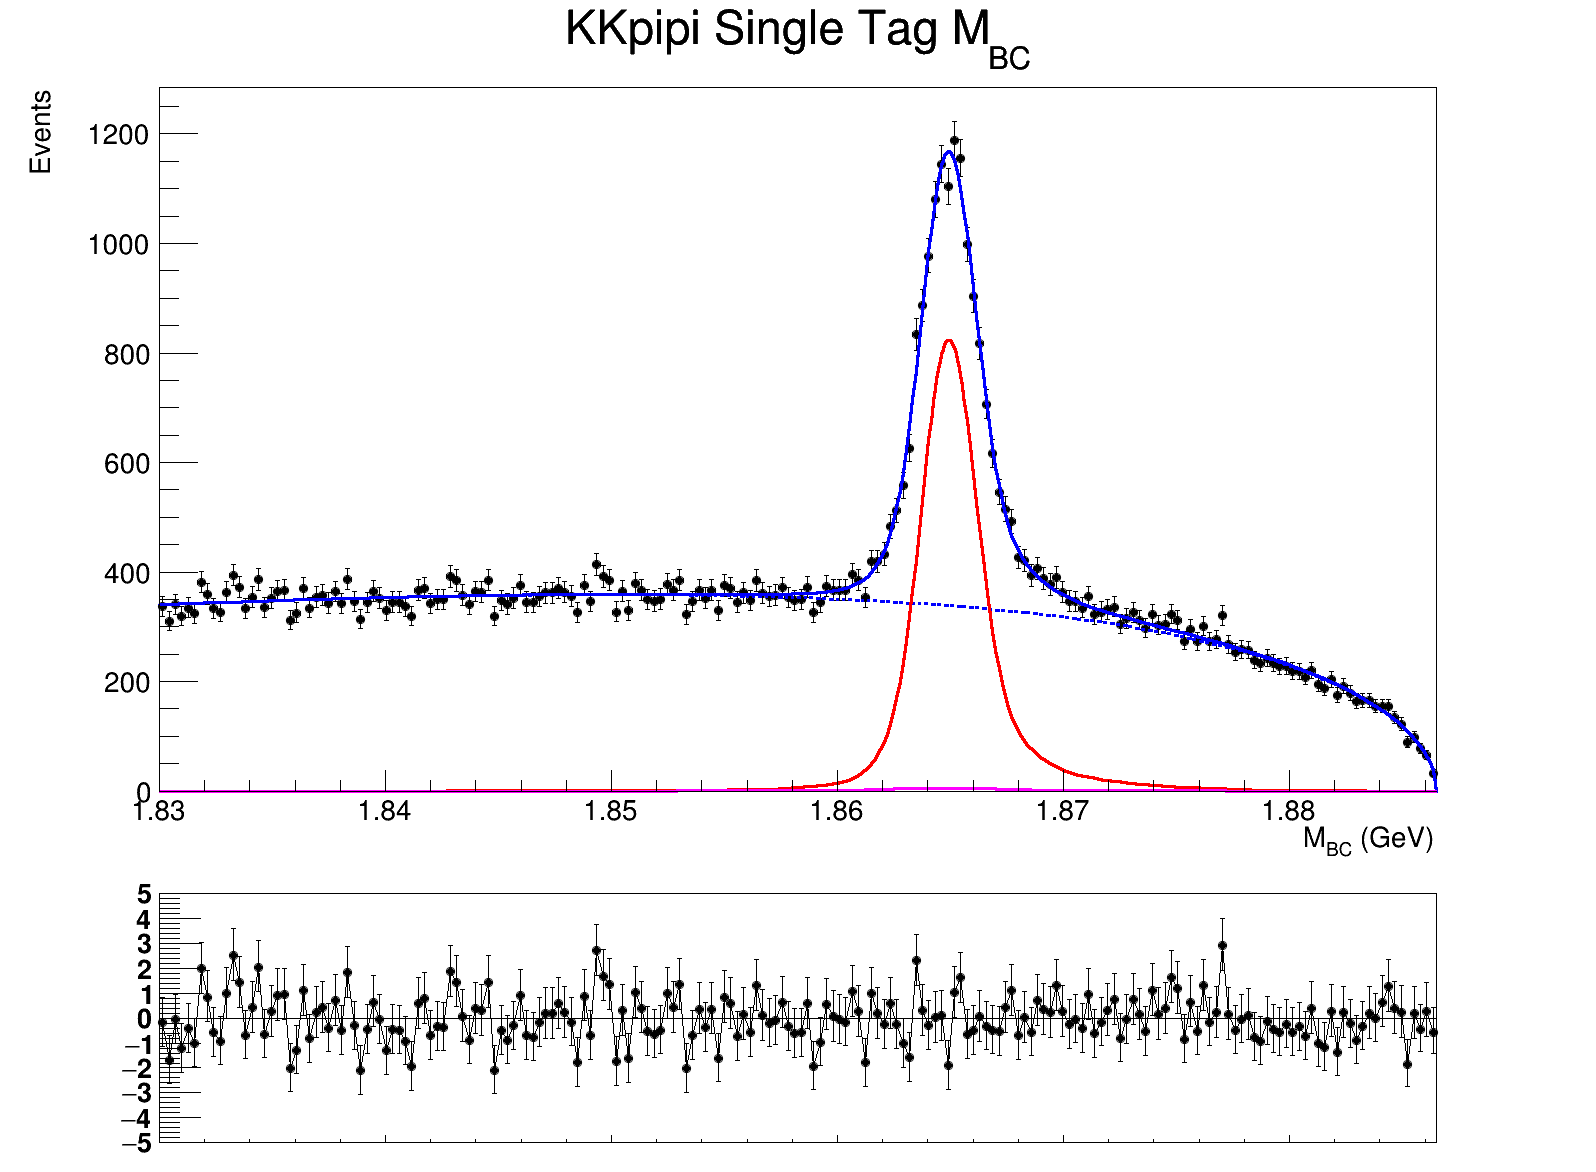
\includegraphics[width=0.85\textwidth]{Plots/KKpipi_SingleTag_MBC_Plot.png}
      \caption{$KK\pi\pi$}
    \end{subfigure}%
    \begin{subfigure}{0.5\textwidth}
      \centering
      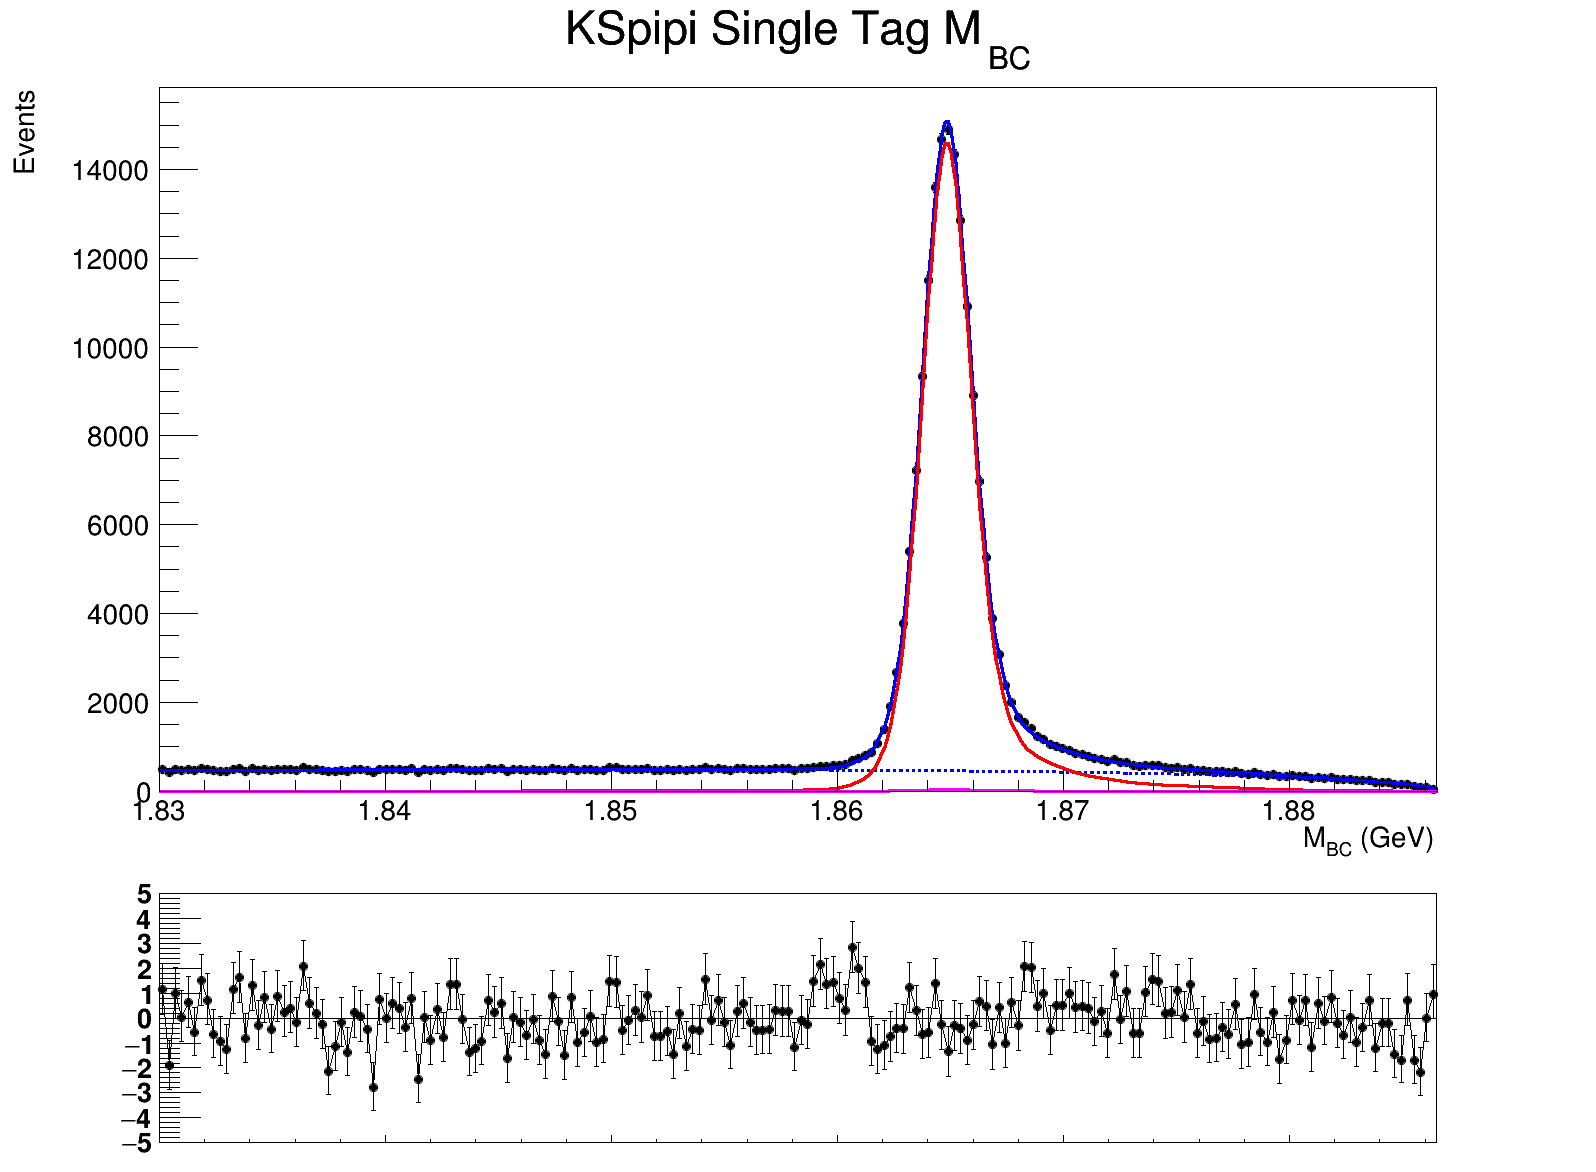
\includegraphics[width=0.85\textwidth]{Plots/KSpipi_SingleTag_MBC_Plot.png}
      \caption{$K_S\pi\pi$}
    \end{subfigure}
  \end{figure}
\end{frame}

\begin{frame}{Single tag fits}
  \begin{figure}
    \centering
    \begin{subfigure}{0.33\textwidth}
      \centering
      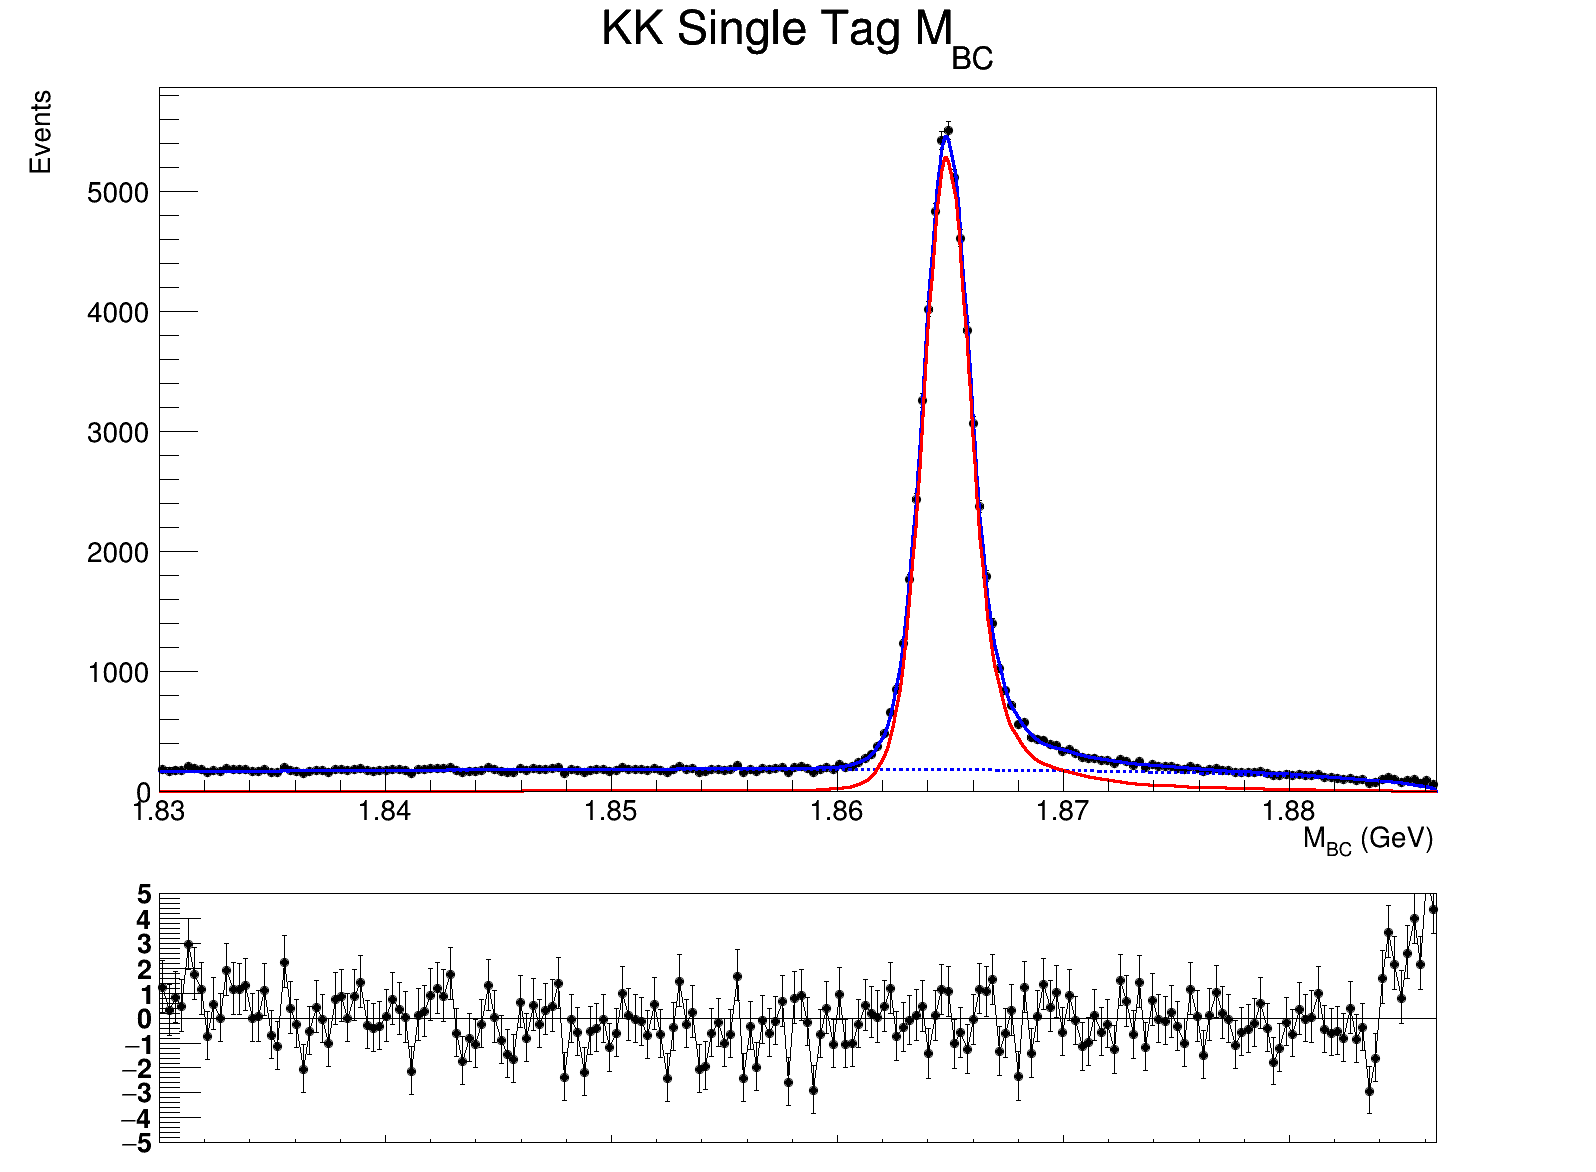
\includegraphics[width=1.0\textwidth]{Plots/KK_SingleTag_MBC_Plot.png}
      \caption{$KK$}
    \end{subfigure}%
    \begin{subfigure}{0.33\textwidth}
      \centering
      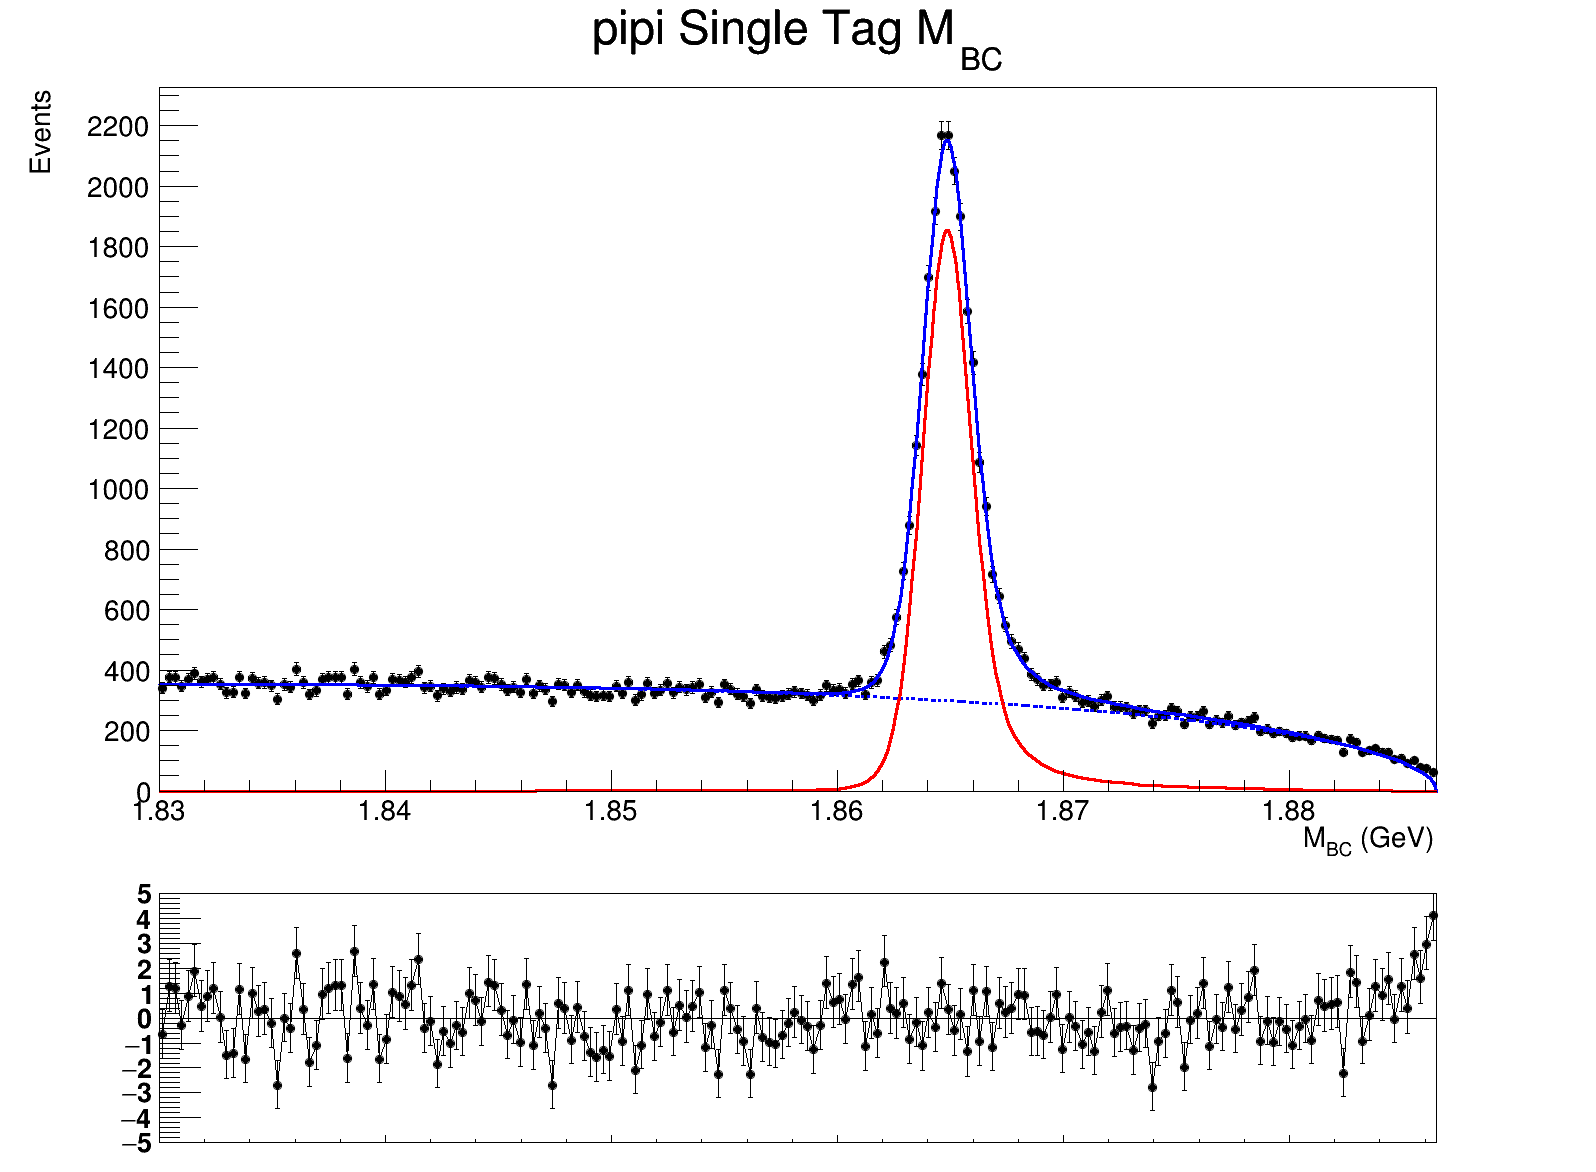
\includegraphics[width=1.0\textwidth]{Plots/pipi_SingleTag_MBC_Plot.png}
      \caption{$\pi\pi$}
    \end{subfigure}
    \begin{subfigure}{0.33\textwidth}
      \centering
      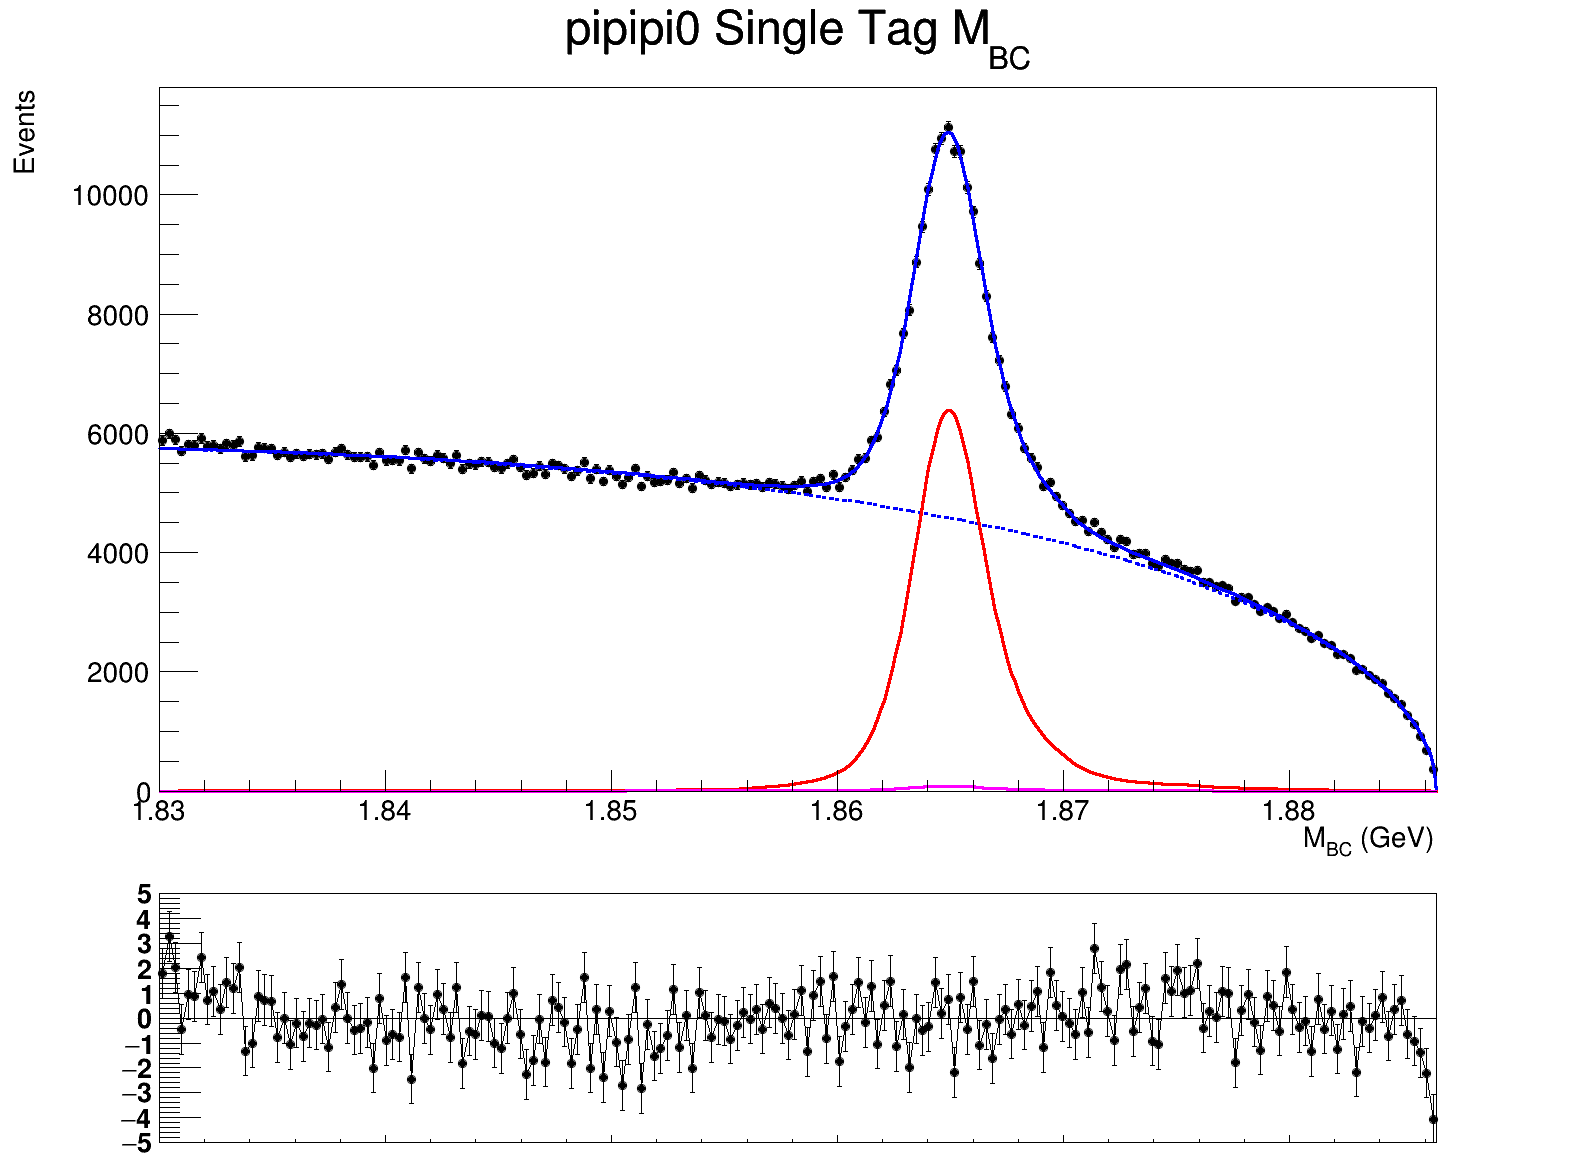
\includegraphics[width=1.0\textwidth]{Plots/pipipi0_SingleTag_MBC_Plot.png}
      \caption{$\pi\pi\pi^0$}
    \end{subfigure}%
    \begin{subfigure}{0.33\textwidth}
      \centering
      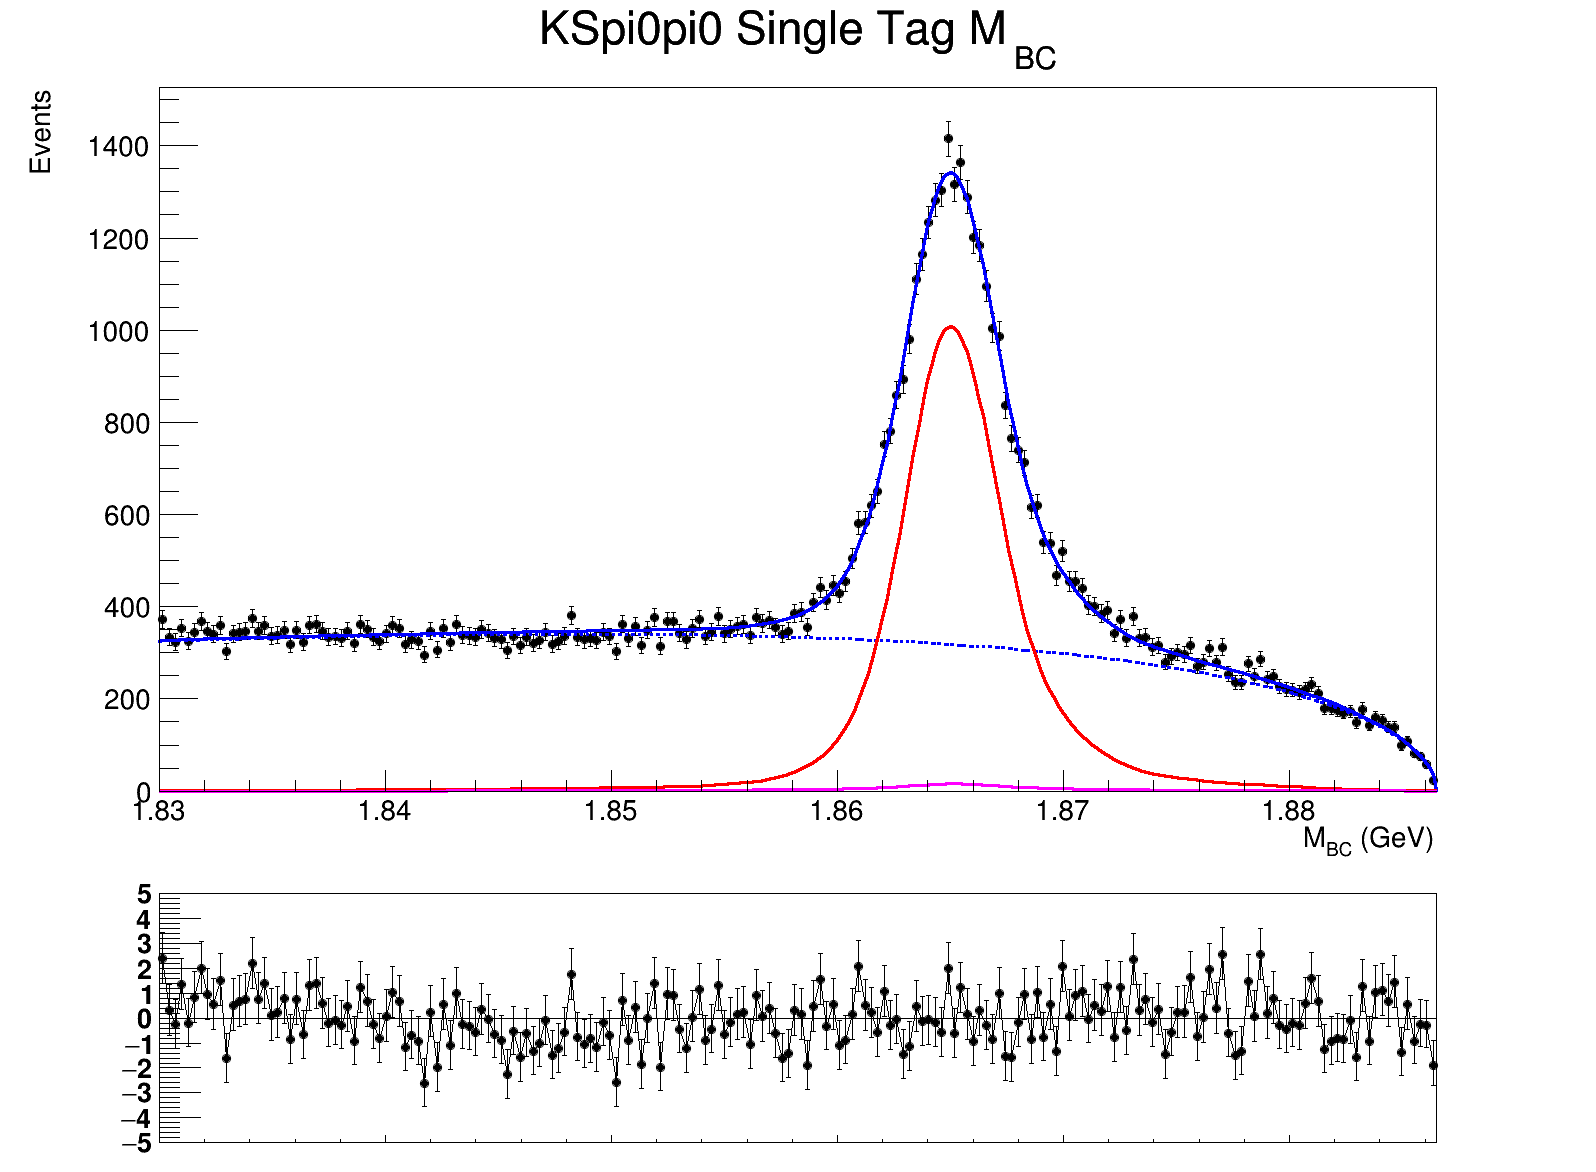
\includegraphics[width=1.0\textwidth]{Plots/KSpi0pi0_SingleTag_MBC_Plot.png}
      \caption{$K_S\pi^0\pi^0$}
    \end{subfigure}
    \caption{Single tag fits of CP even tags}
  \end{figure}
\end{frame}

\begin{frame}{Single tag fits}
  \begin{figure}
    \centering
    \begin{subfigure}{0.33\textwidth}
      \centering
      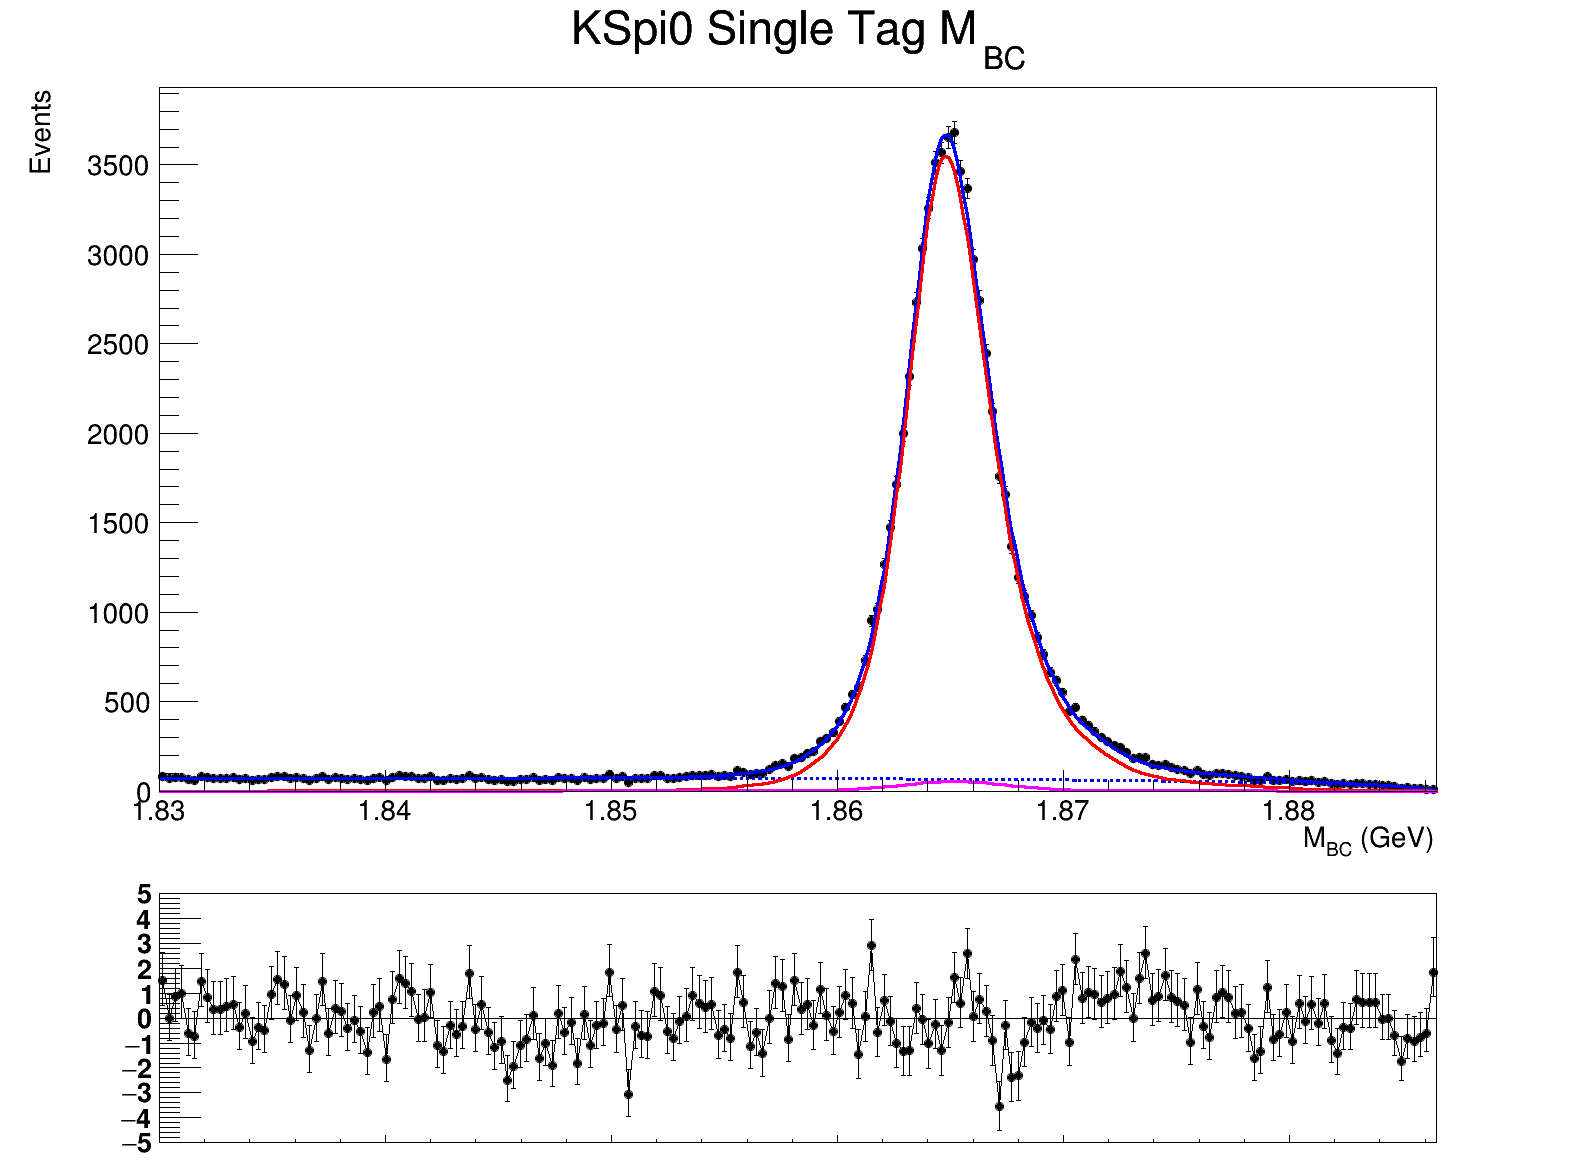
\includegraphics[width=1.0\textwidth]{Plots/KSpi0_SingleTag_MBC_Plot.png}
      \caption{$K_S\pi^0$}
    \end{subfigure}%
    \begin{subfigure}{0.33\textwidth}
      \centering
      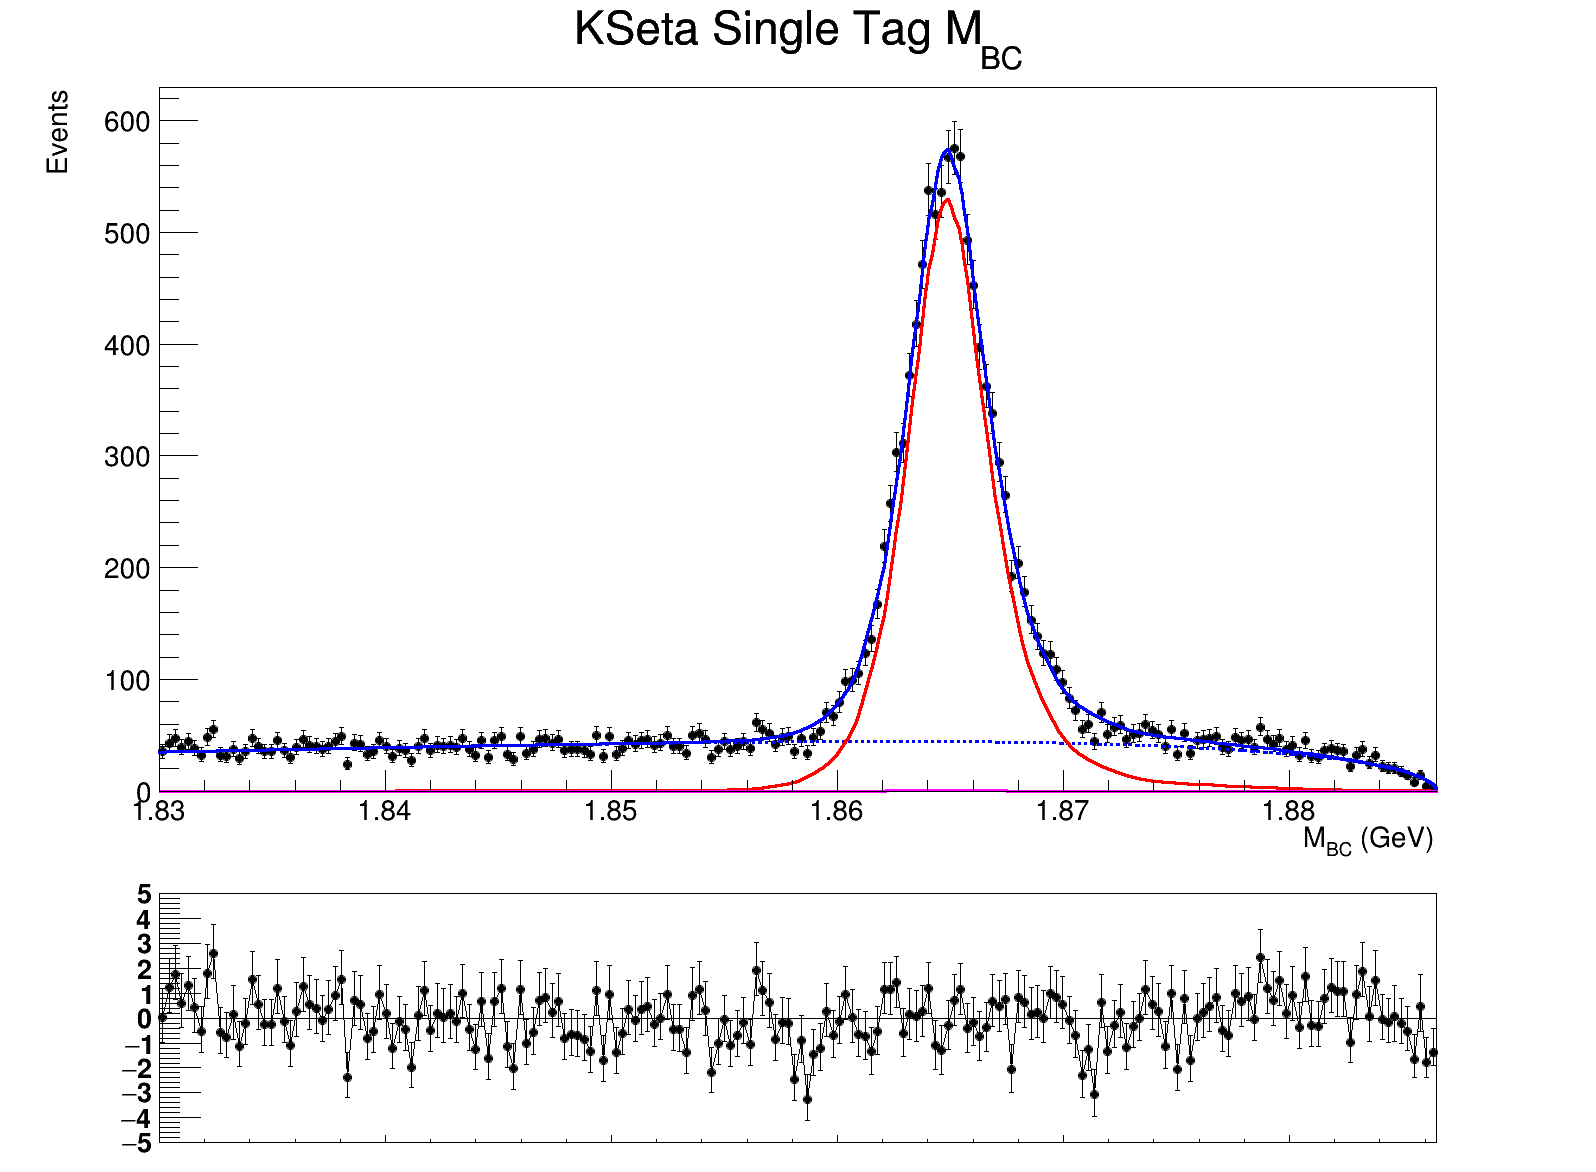
\includegraphics[width=1.0\textwidth]{Plots/KSeta_SingleTag_MBC_Plot.png}
      \caption{$K_S\eta$}
    \end{subfigure}
    \begin{subfigure}{0.33\textwidth}
      \centering
      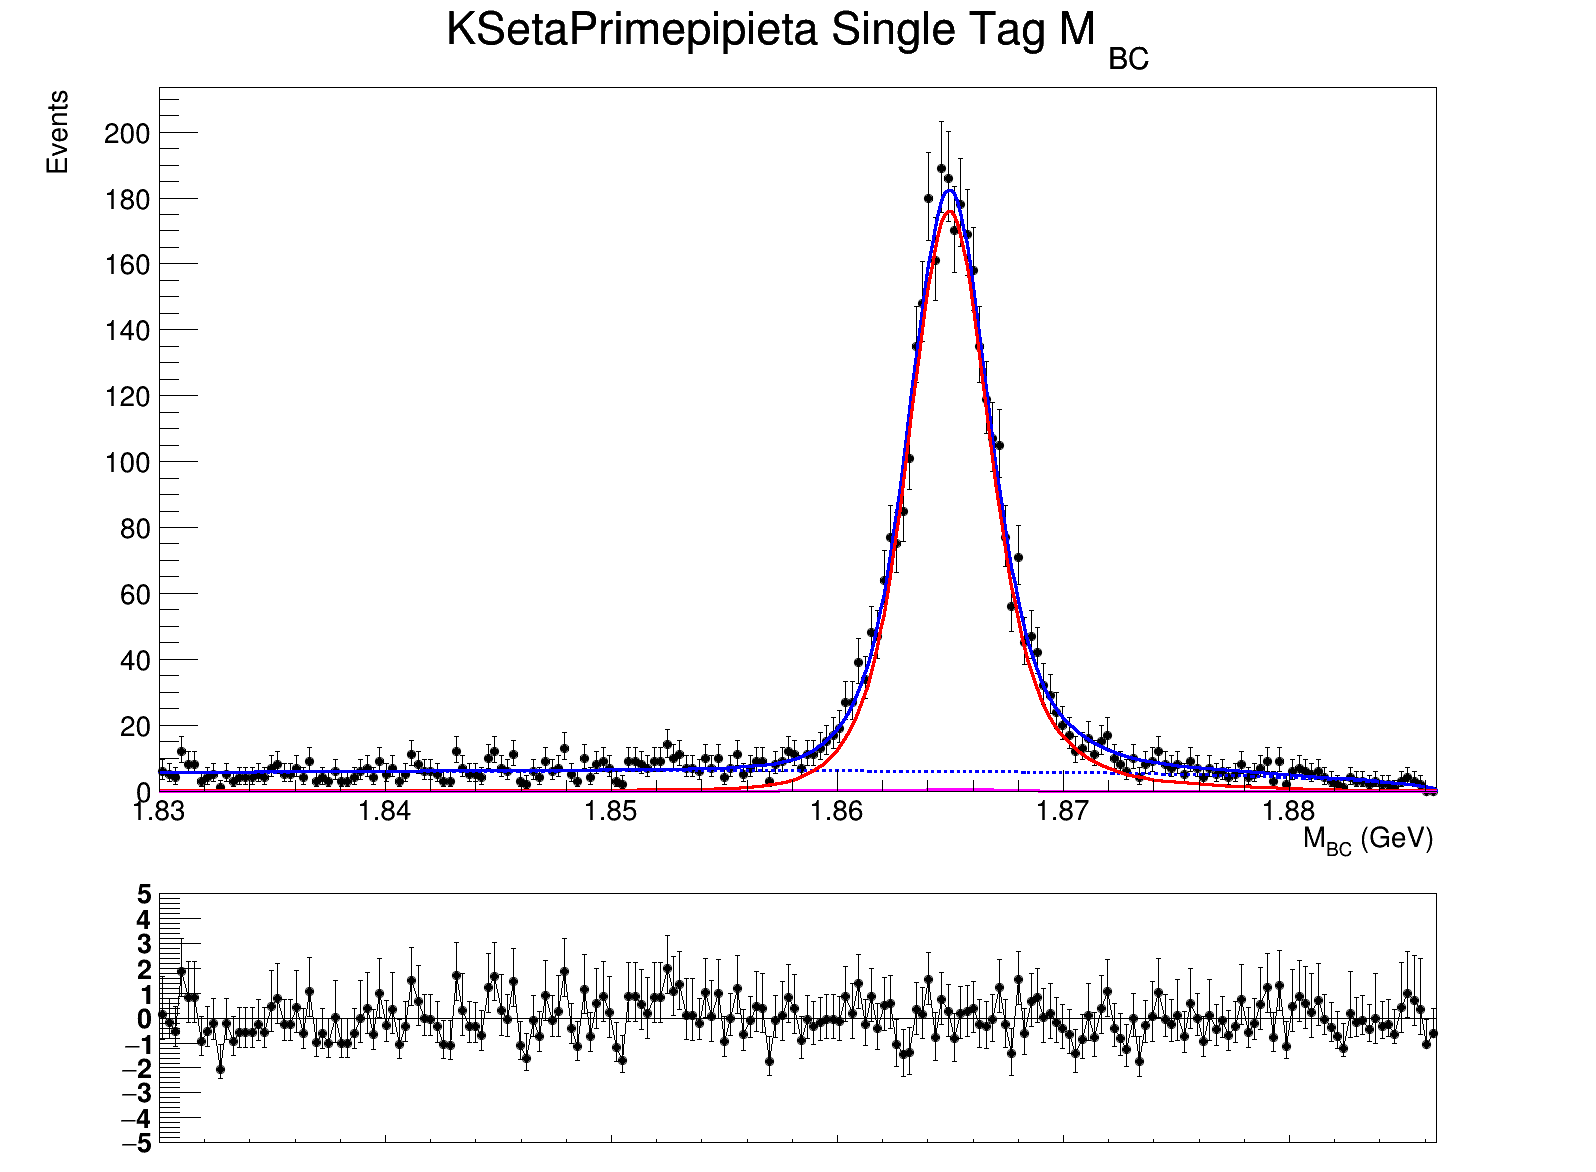
\includegraphics[width=1.0\textwidth]{Plots/KSetaPrimepipieta_SingleTag_MBC_Plot.png}
      \caption{$K_S\eta^\prime(\pi\pi\eta)$}
    \end{subfigure}%
    \begin{subfigure}{0.33\textwidth}
      \centering
      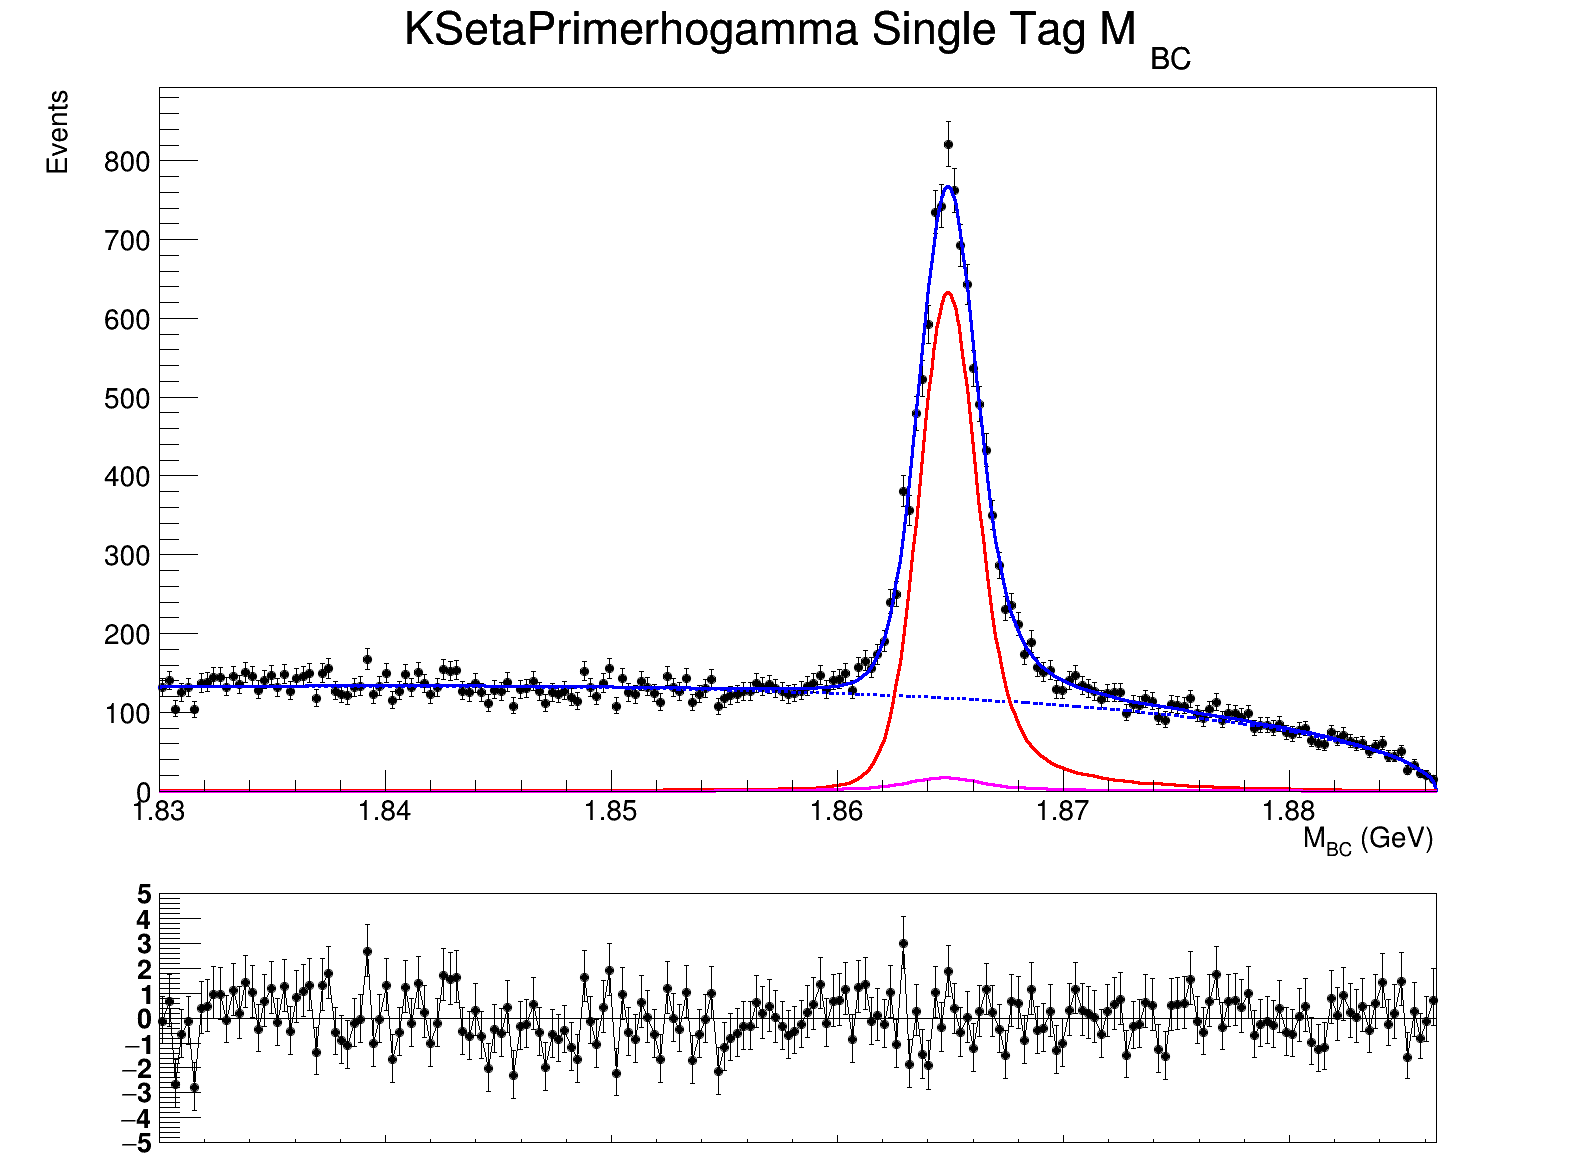
\includegraphics[width=1.0\textwidth]{Plots/KSetaPrimerhogamma_SingleTag_MBC_Plot.png}
      \caption{$K_S\eta^\prime(\rho\gamma)$}
    \end{subfigure}%
    \begin{subfigure}{0.33\textwidth}
      \centering
      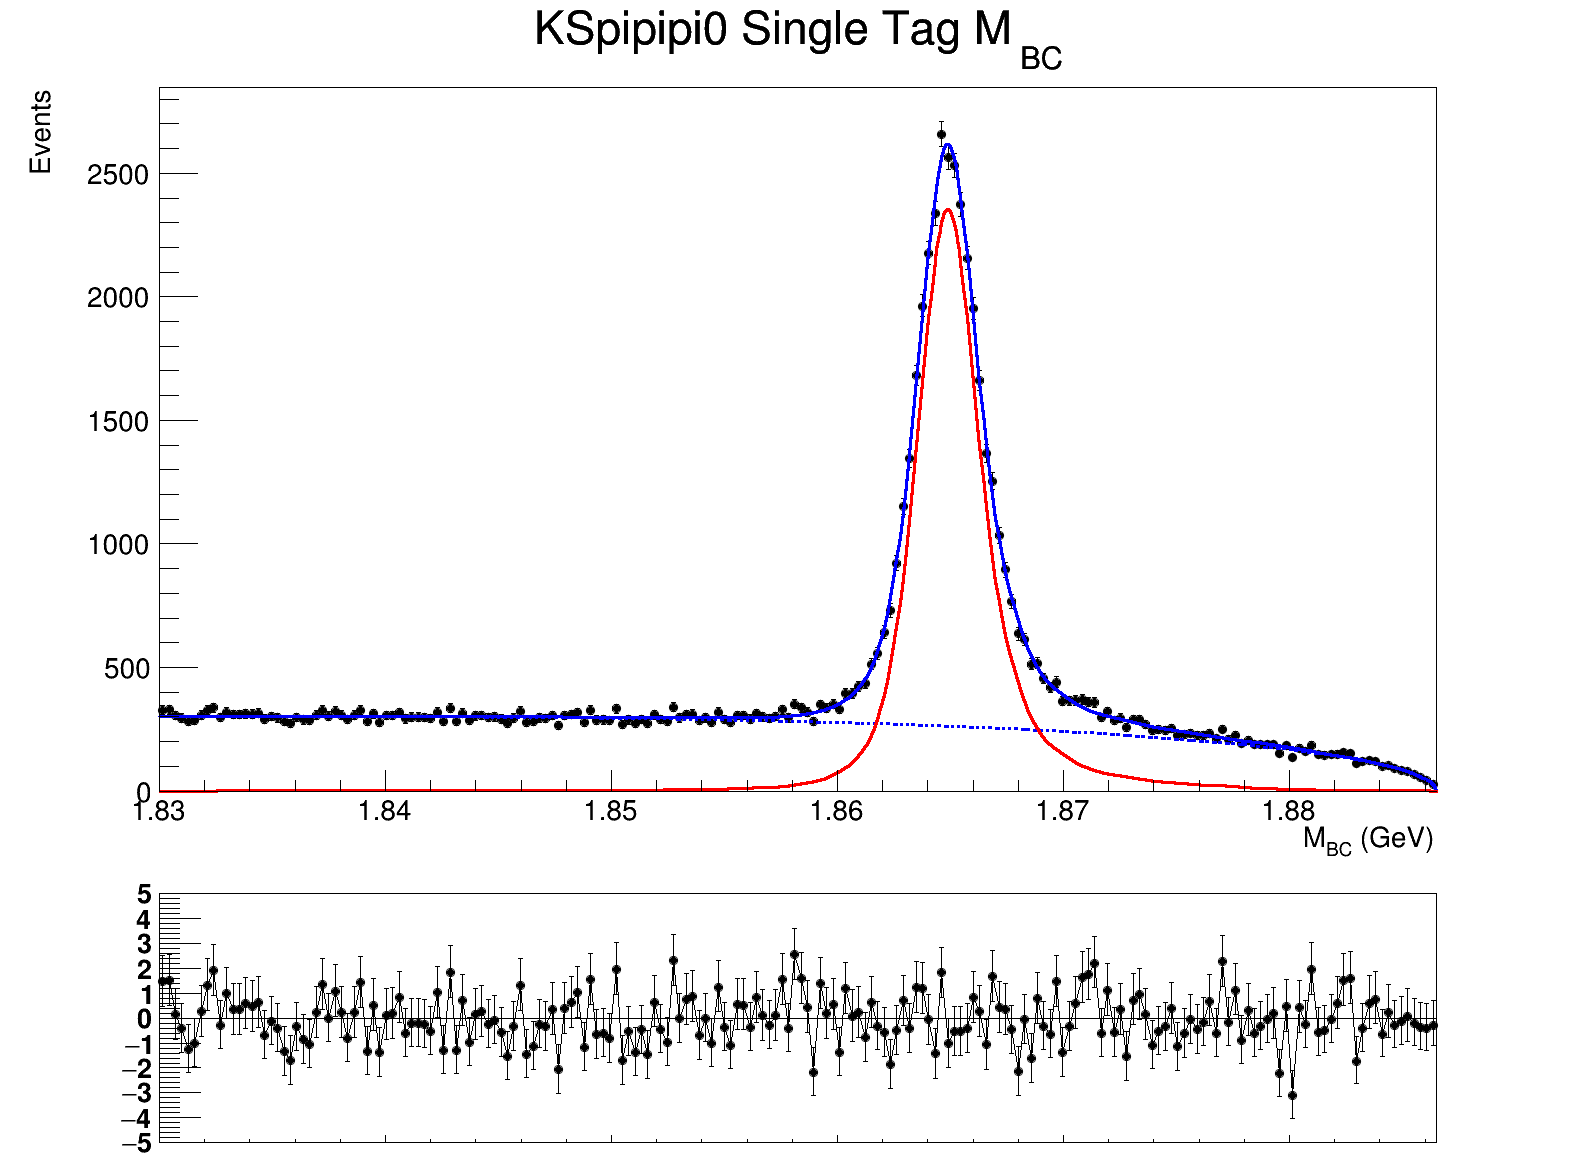
\includegraphics[width=1.0\textwidth]{Plots/KSpipipi0_SingleTag_MBC_Plot.png}
      \caption{$K_S\omega$}
    \end{subfigure}
    \caption{Single tag fits of CP odd tags}
  \end{figure}
\end{frame}

\begin{frame}{Single tag yields and efficiencies}
  \begin{center}
    \begin{tabular}{lcc}
      Tag mode                          & Single tag yield     & Single tag efficiency ($\%$) \\
      \hline
      $K^+K^-\pi^+\pi^-$                & $10642 \pm 156$      & $19.02 \pm 0.09$     \\
      \hline
      $K^+K^-$                          & $56303 \pm 262$      & $63.41 \pm 0.11$     \\
      $\pi^+\pi^-$                      & $20386 \pm 179$      & $67.41 \pm 0.10$     \\
      $K_S\pi^0$                        & $67876 \pm 278$      & $38.18 \pm 0.11$     \\
      $K_S\pi^0\pi^0$                   & $22392 \pm 229$      & $14.35 \pm 0.08$     \\
      $K_L\pi^0$                        & $47595 \pm 1653$     & $27.83 \pm 0.23$     \\
      \hline
      $K_S\eta$                         & $9308 \pm 113$       & $31.78 \pm 0.10$     \\
      $K_S\eta^\prime_{\pi\pi\eta}$     & $3213 \pm 62$        & $12.81 \pm 0.07$     \\
      $K_S\eta^\prime_{\rho\gamma}$     & $8283 \pm 116$       & $20.80 \pm 0.09$     \\
      $\pi^+\pi^-\pi^0$                 & $107504 \pm 602$     & $36.65 \pm 0.11$     \\
      $K_S\omega$                       & $22068 \pm 217$      & $14.50 \pm 0.08$     \\
      \hline
      $K_S\pi^+\pi^-$                   & $161914 \pm 440$     & $36.40 \pm 0.11$     \\
      $K_S\pi^+\pi^-$ part. reco.       & $161914 \pm 440$     & $36.40 \pm 0.11$     \\
      $K_L\pi^+\pi^-$                   & $223141 \pm 2146$    & $46.1 \pm 0.3$       \\
      \hline
    \end{tabular}
  \end{center}
\end{frame}

\section{Fit of double tag yields}
\subsection{Fit strategy}

\begin{frame}{Double tag fits}
  \begin{itemize}
    \setlength\itemsep{1.0em}
    \item{Fit strategy:}
    \begin{itemize}
      \item{Fully reconstructed tags: Only fit signal $m_{\rm BC}$ because of low statistics}
      \item{Partially reconstructed tags: Fit missing mass squared $m^2_{\rm miss}$}
    \end{itemize}
    \item{Fit model:}
    \begin{itemize}
      \item{Signal: PDF from signal MC, convoluted with single Gaussian}
      \item{Background: Argus PDF}
      \item{Peaking backgrounds fixed, with quantum correlation accounted for}
      \item{Simple sideband subtraction for correct signal but wrong tag event}
    \end{itemize}
    \item{For tags with multiple bins, perform a simultaneous fit of all bins}
    \begin{itemize}
      \item{Shape is floated and shared across all bins}
      \item{Yield of signal and combinatorial background is floated in each bin}
    \end{itemize}
  \end{itemize}
\end{frame}

\subsection{CP tags}

\begin{frame}{Double tag fits}
  \begin{figure}
    \centering
    \begin{subfigure}{0.33\textwidth}
      \centering
      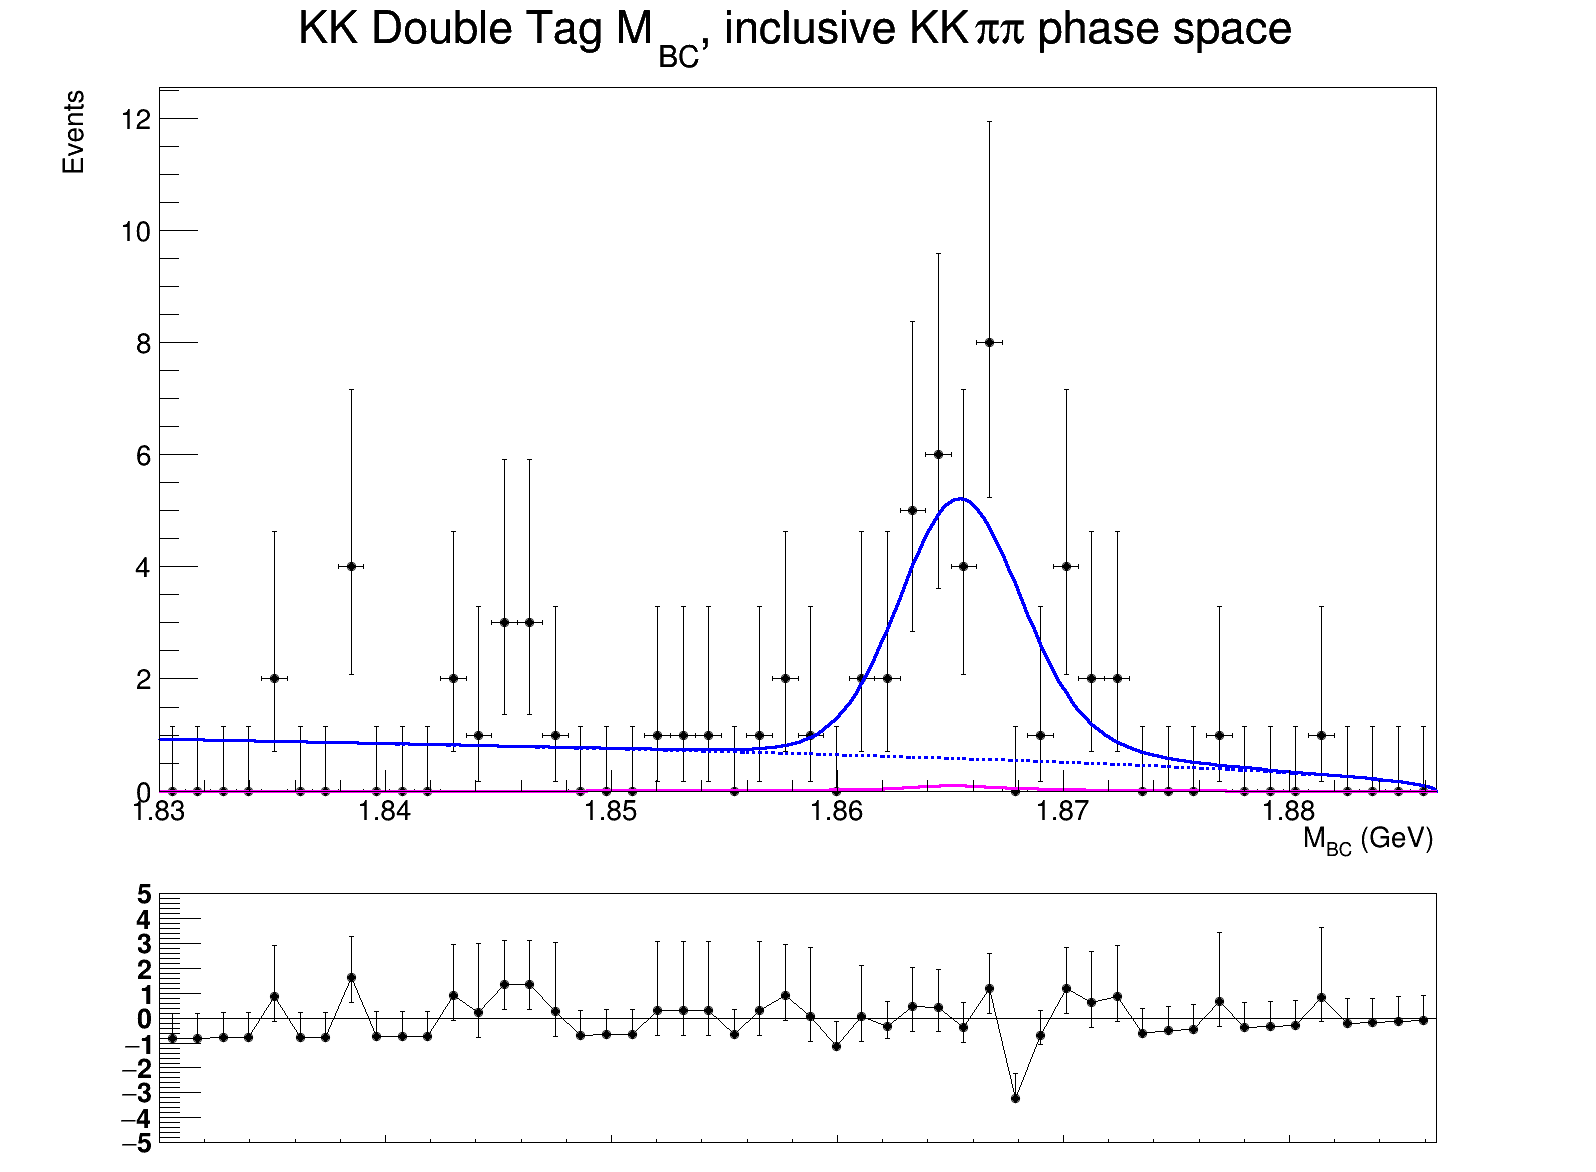
\includegraphics[width=1.0\textwidth]{Plots/DoubleTagYield_DoubleTag_CP_KKpipi_vs_KK_SignalBin0.png}
      \caption{$KK$}
    \end{subfigure}%
    \begin{subfigure}{0.33\textwidth}
      \centering
      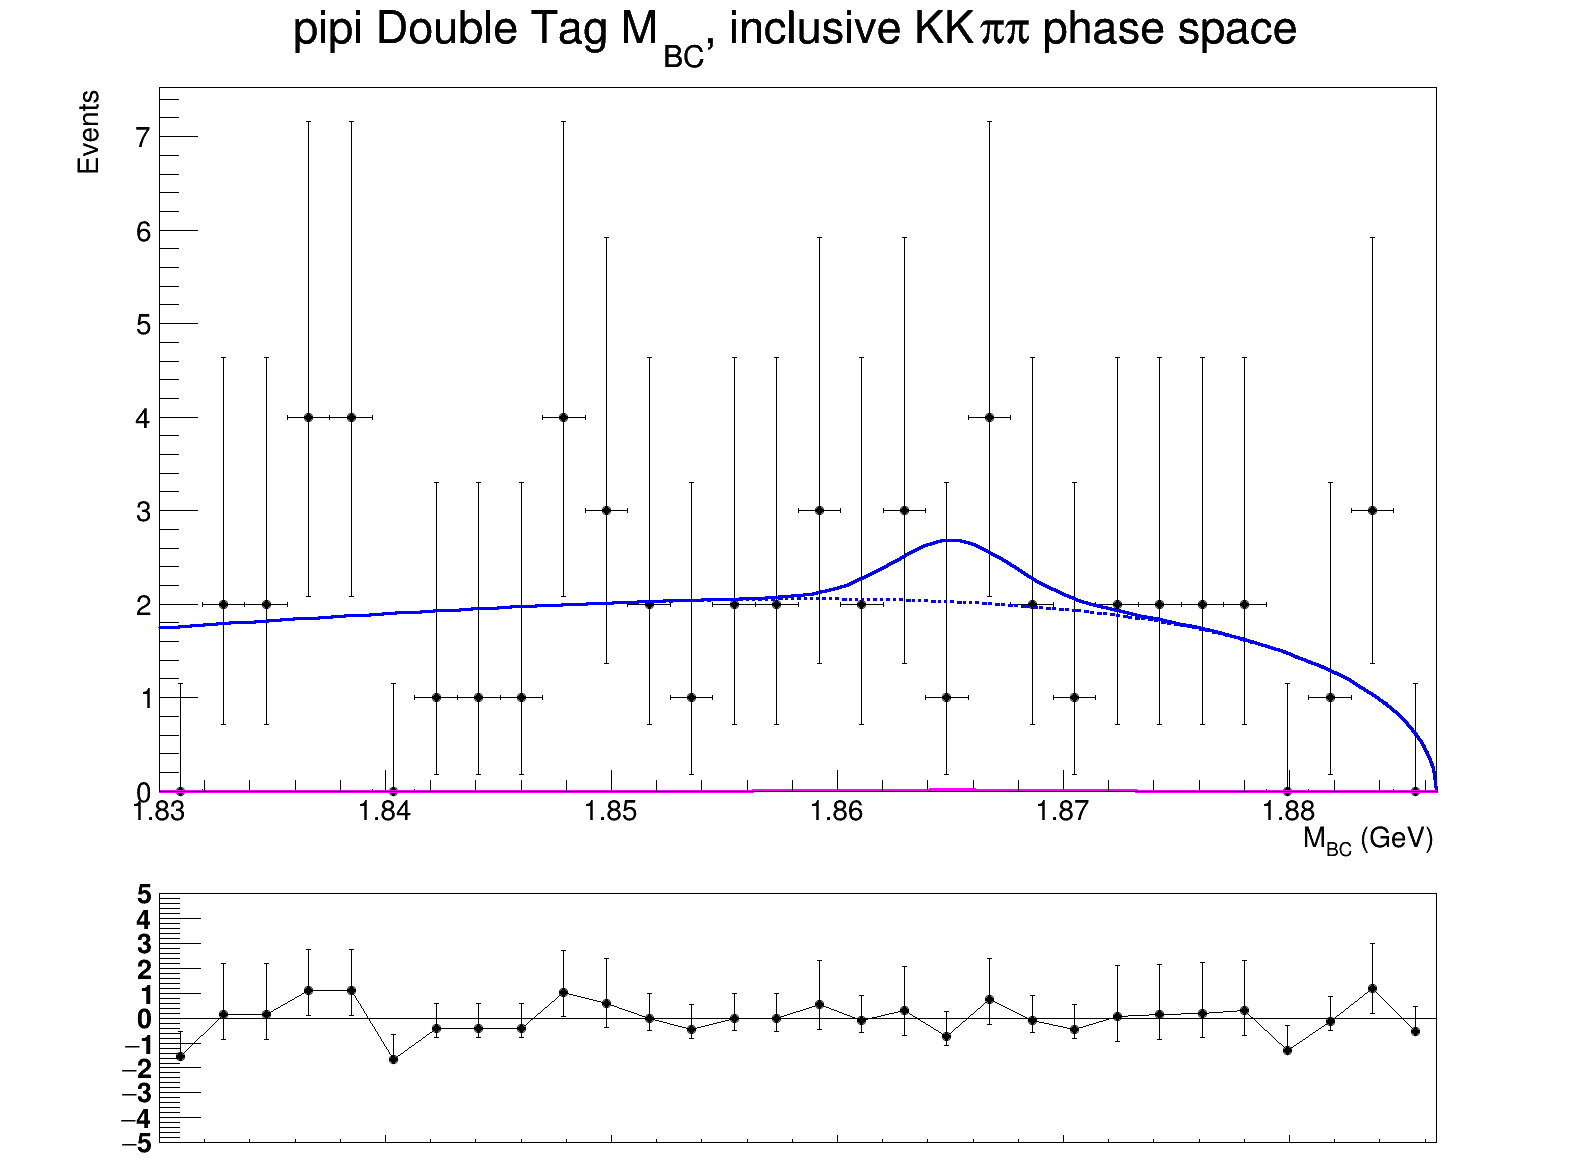
\includegraphics[width=1.0\textwidth]{Plots/DoubleTagYield_DoubleTag_CP_KKpipi_vs_pipi_SignalBin0.png}
      \caption{$\pi\pi$}
    \end{subfigure}
    \begin{subfigure}{0.33\textwidth}
      \centering
      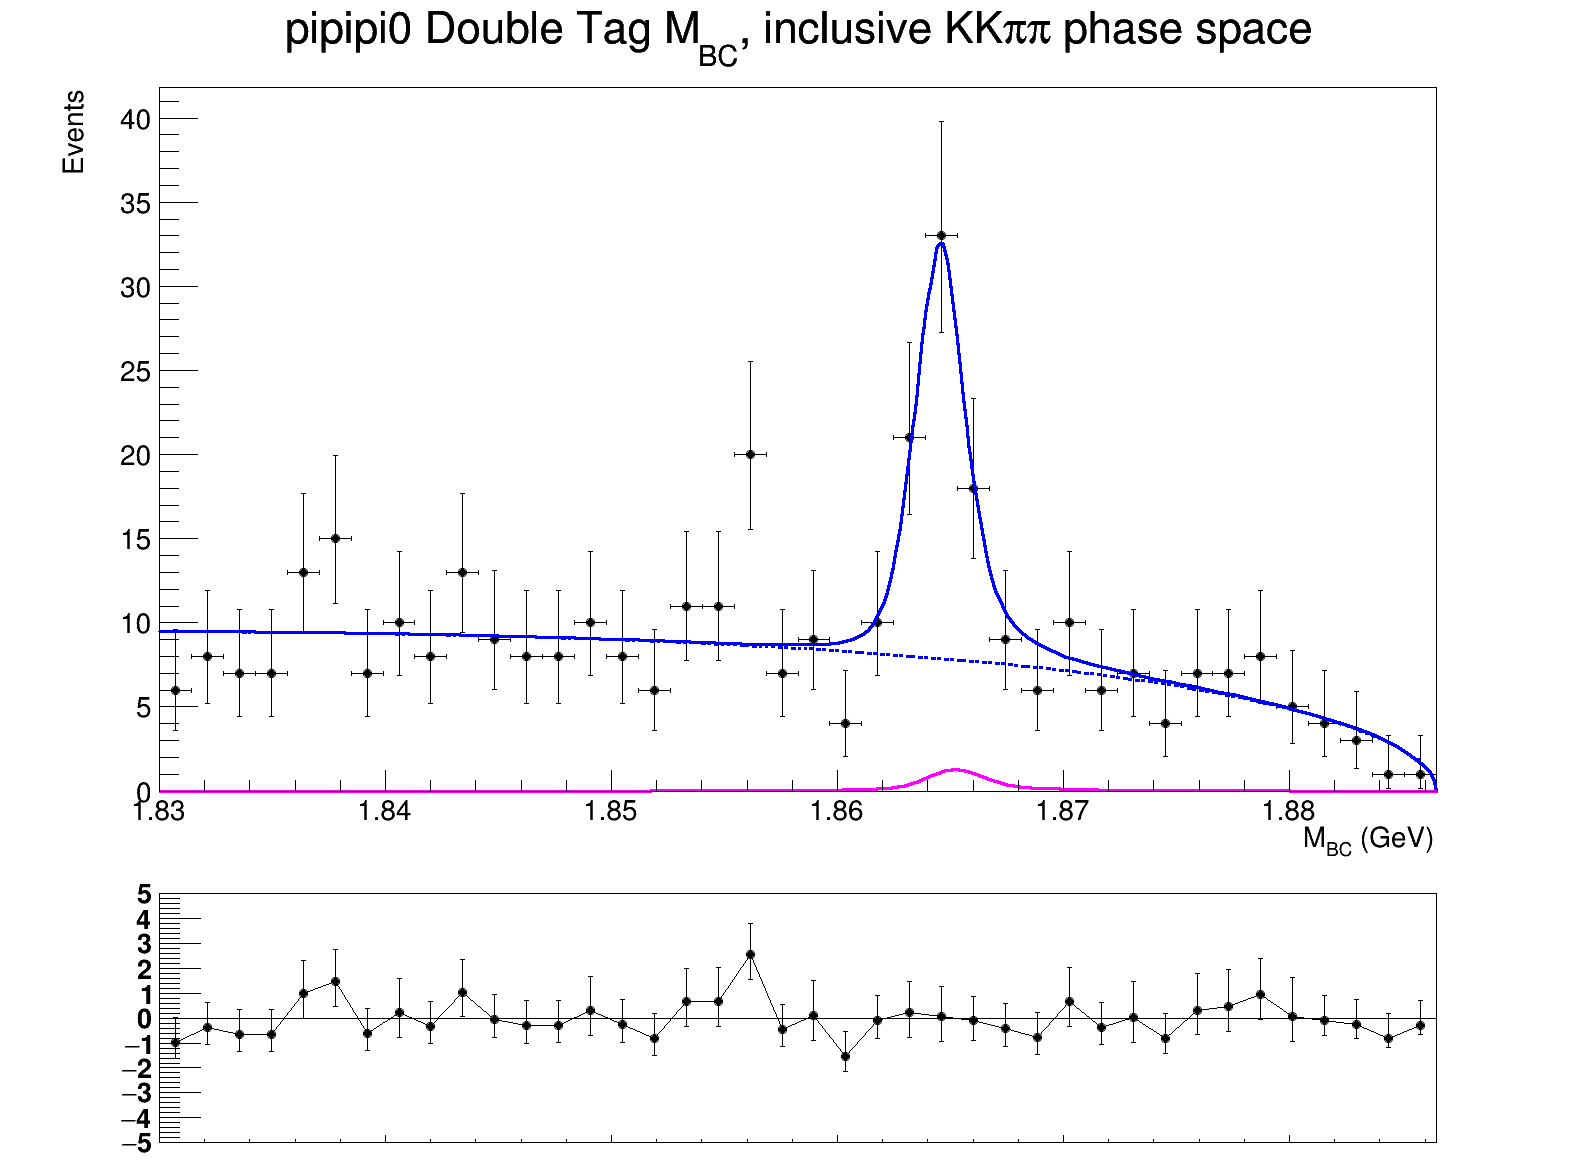
\includegraphics[width=1.0\textwidth]{Plots/DoubleTagYield_DoubleTag_CP_KKpipi_vs_pipipi0_SignalBin0.png}
      \caption{$\pi\pi\pi^0$}
    \end{subfigure}%
    \begin{subfigure}{0.33\textwidth}
      \centering
      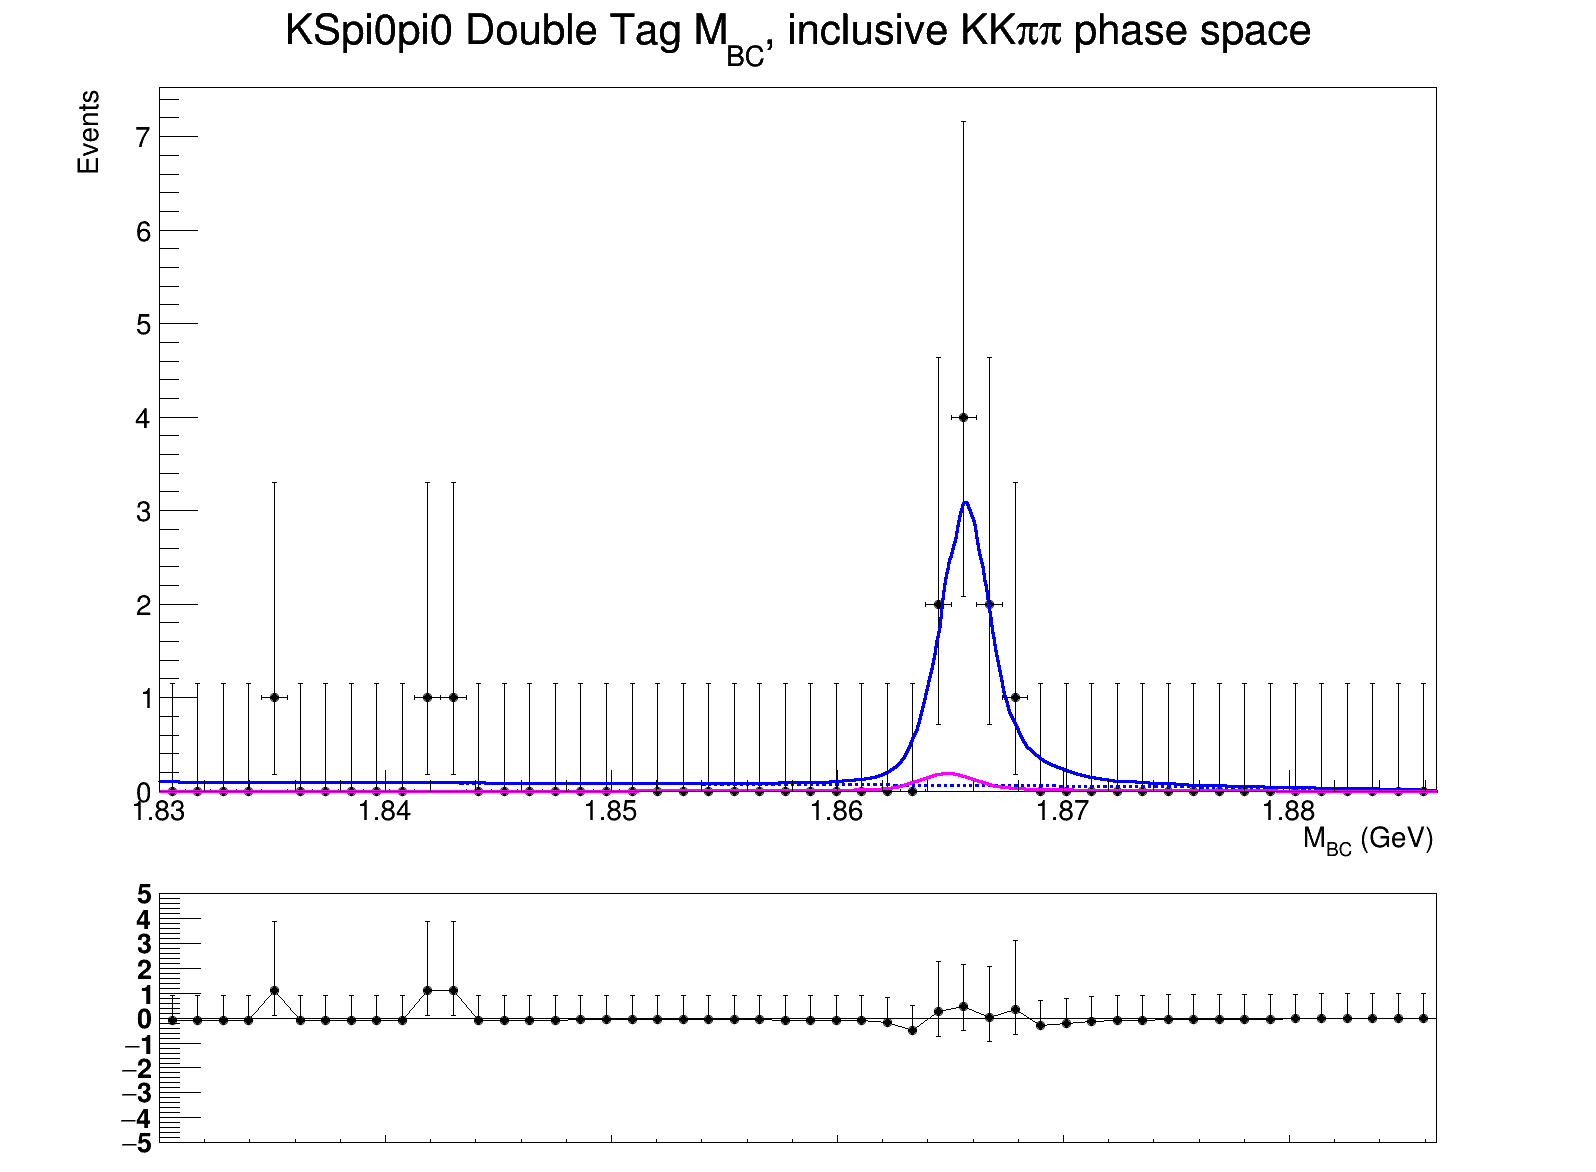
\includegraphics[width=1.0\textwidth]{Plots/DoubleTagYield_DoubleTag_CP_KKpipi_vs_KSpi0pi0_SignalBin0.png}
      \caption{$K_S\pi^0\pi^0$}
    \end{subfigure}%
    \begin{subfigure}{0.33\textwidth}
      \centering
      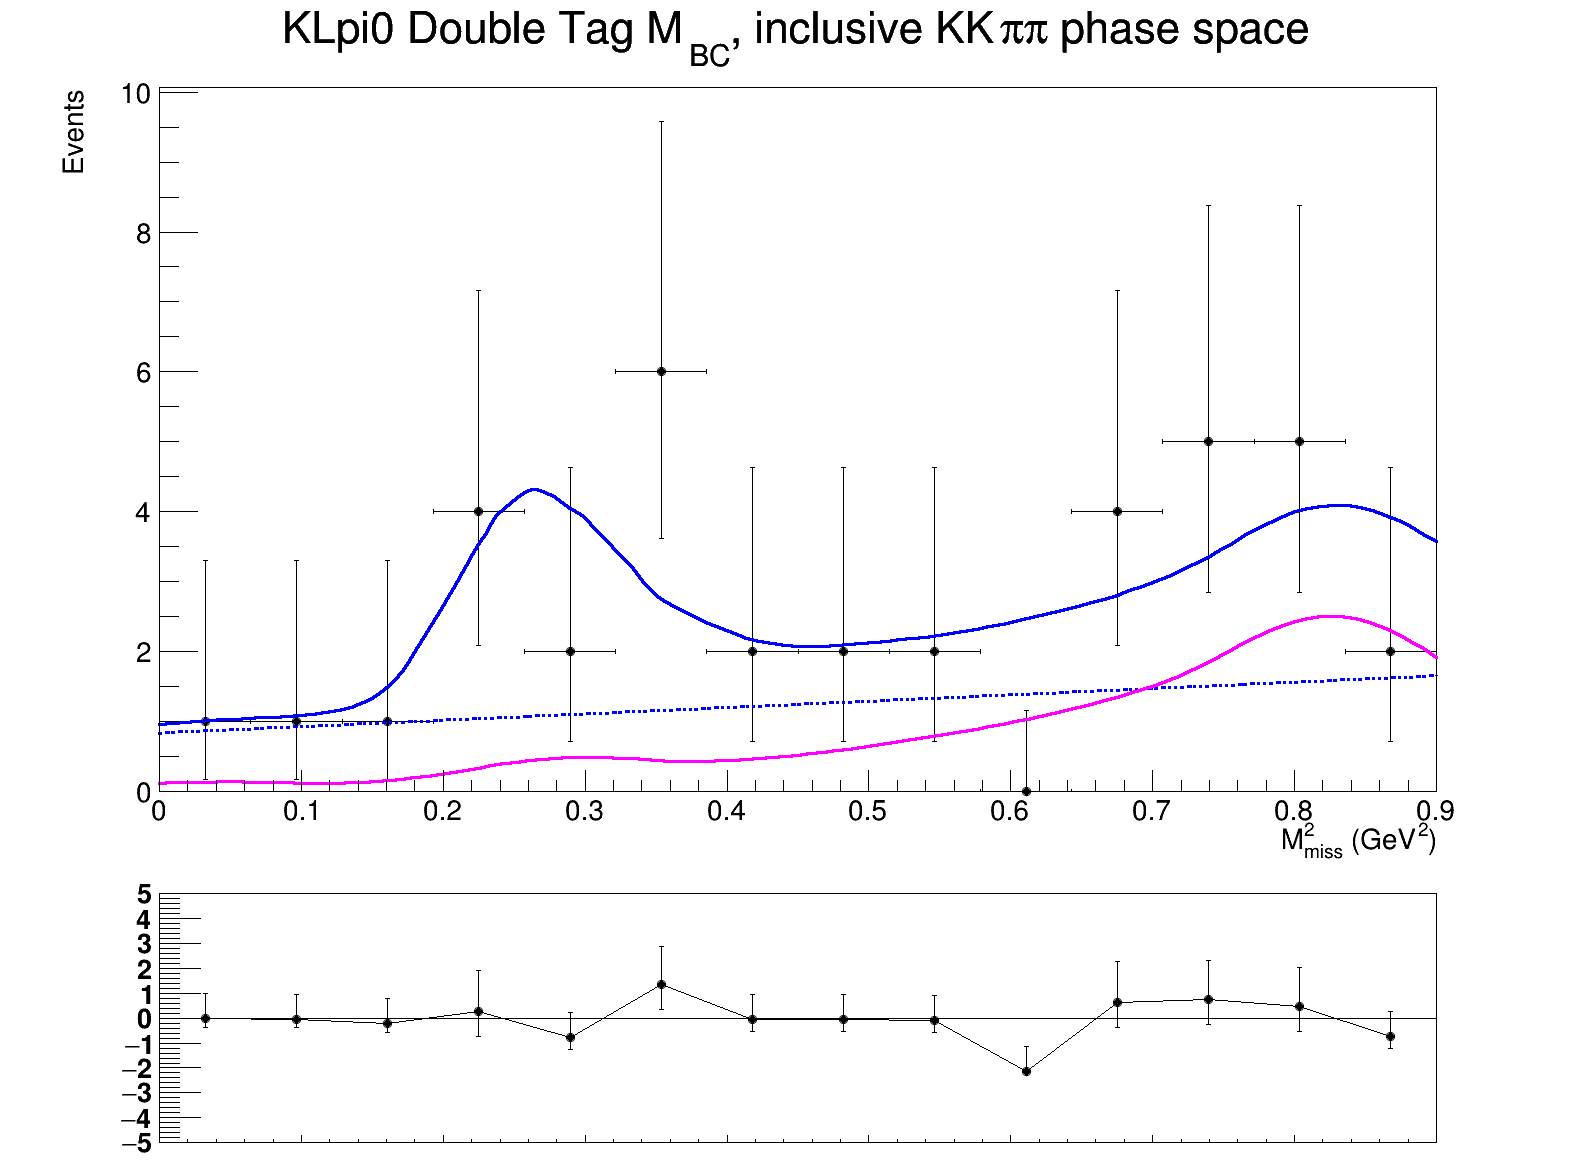
\includegraphics[width=1.0\textwidth]{Plots/DoubleTagYield_DoubleTag_CP_KKpipi_vs_KLpi0_SignalBin0.png}
      \caption{$K_L\pi^0$}
    \end{subfigure}
    \caption{Double tag fits of CP even tags}
  \end{figure}
\end{frame}

\begin{frame}{Double tag fits}
  \begin{figure}
    \centering
    \begin{subfigure}{0.33\textwidth}
      \centering
      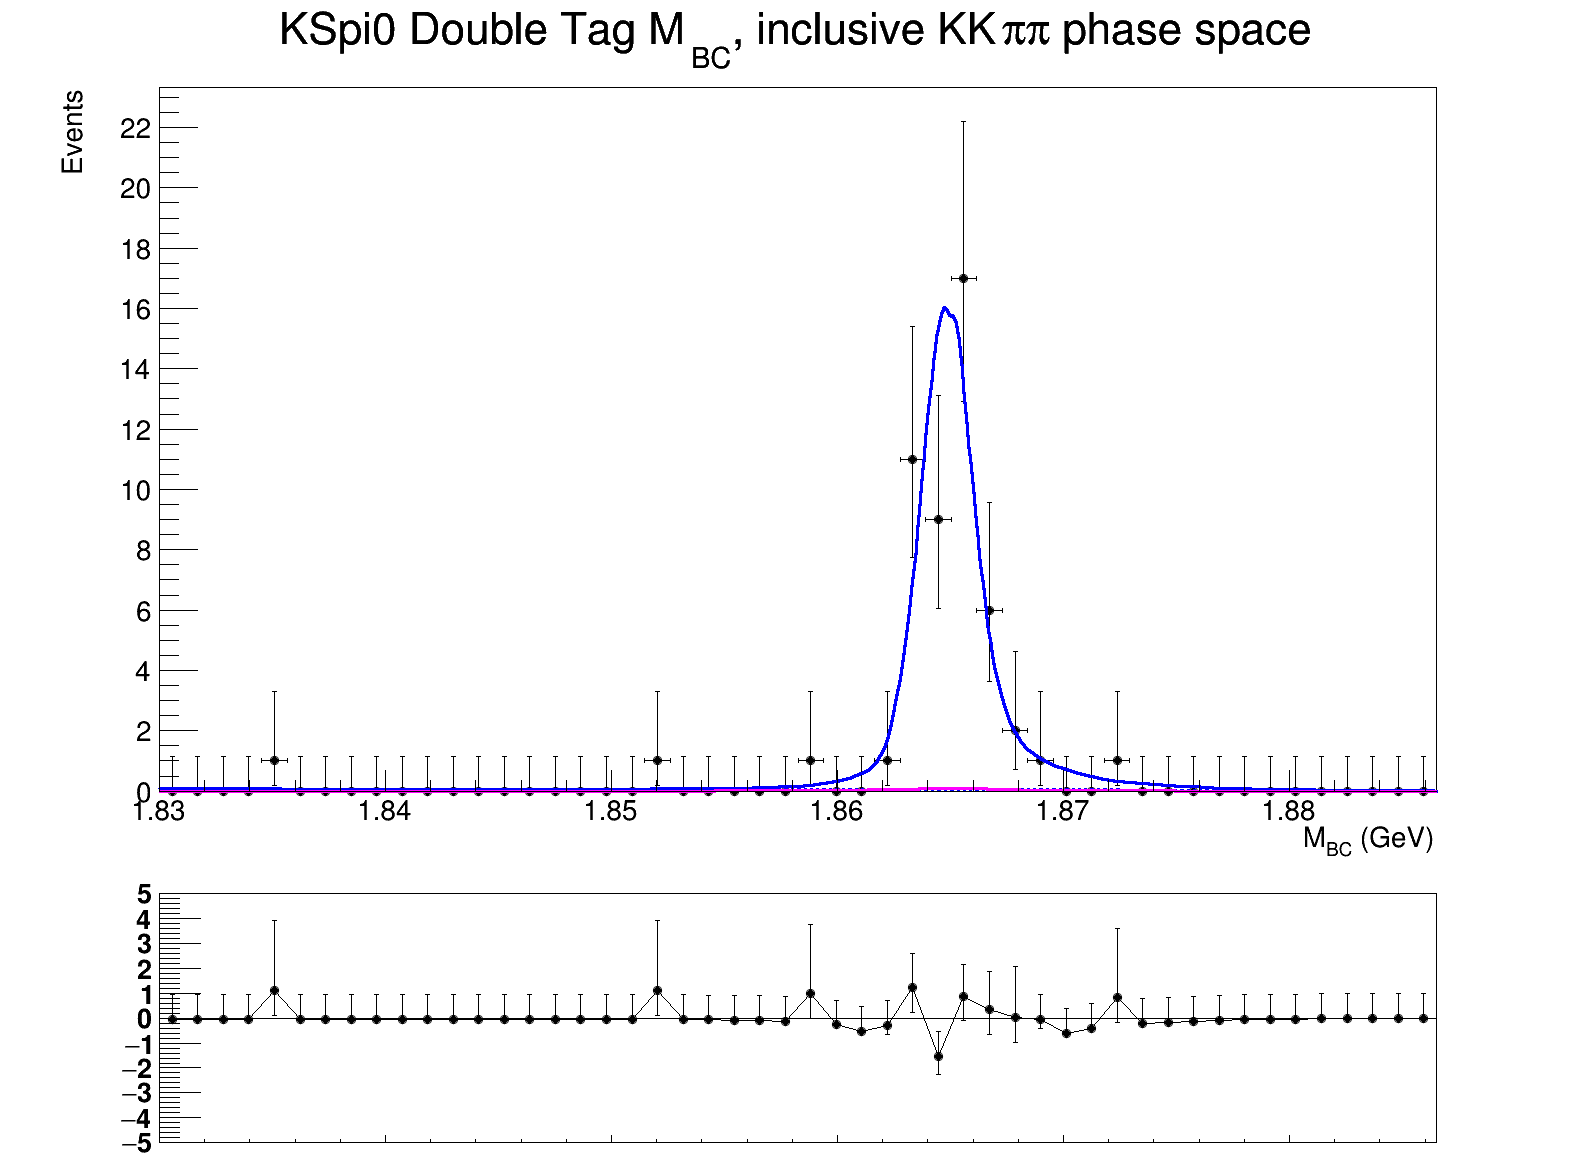
\includegraphics[width=1.0\textwidth]{Plots/DoubleTagYield_DoubleTag_CP_KKpipi_vs_KSpi0_SignalBin0.png}
      \caption{$K_S\pi^0$}
    \end{subfigure}%
    \begin{subfigure}{0.33\textwidth}
      \centering
      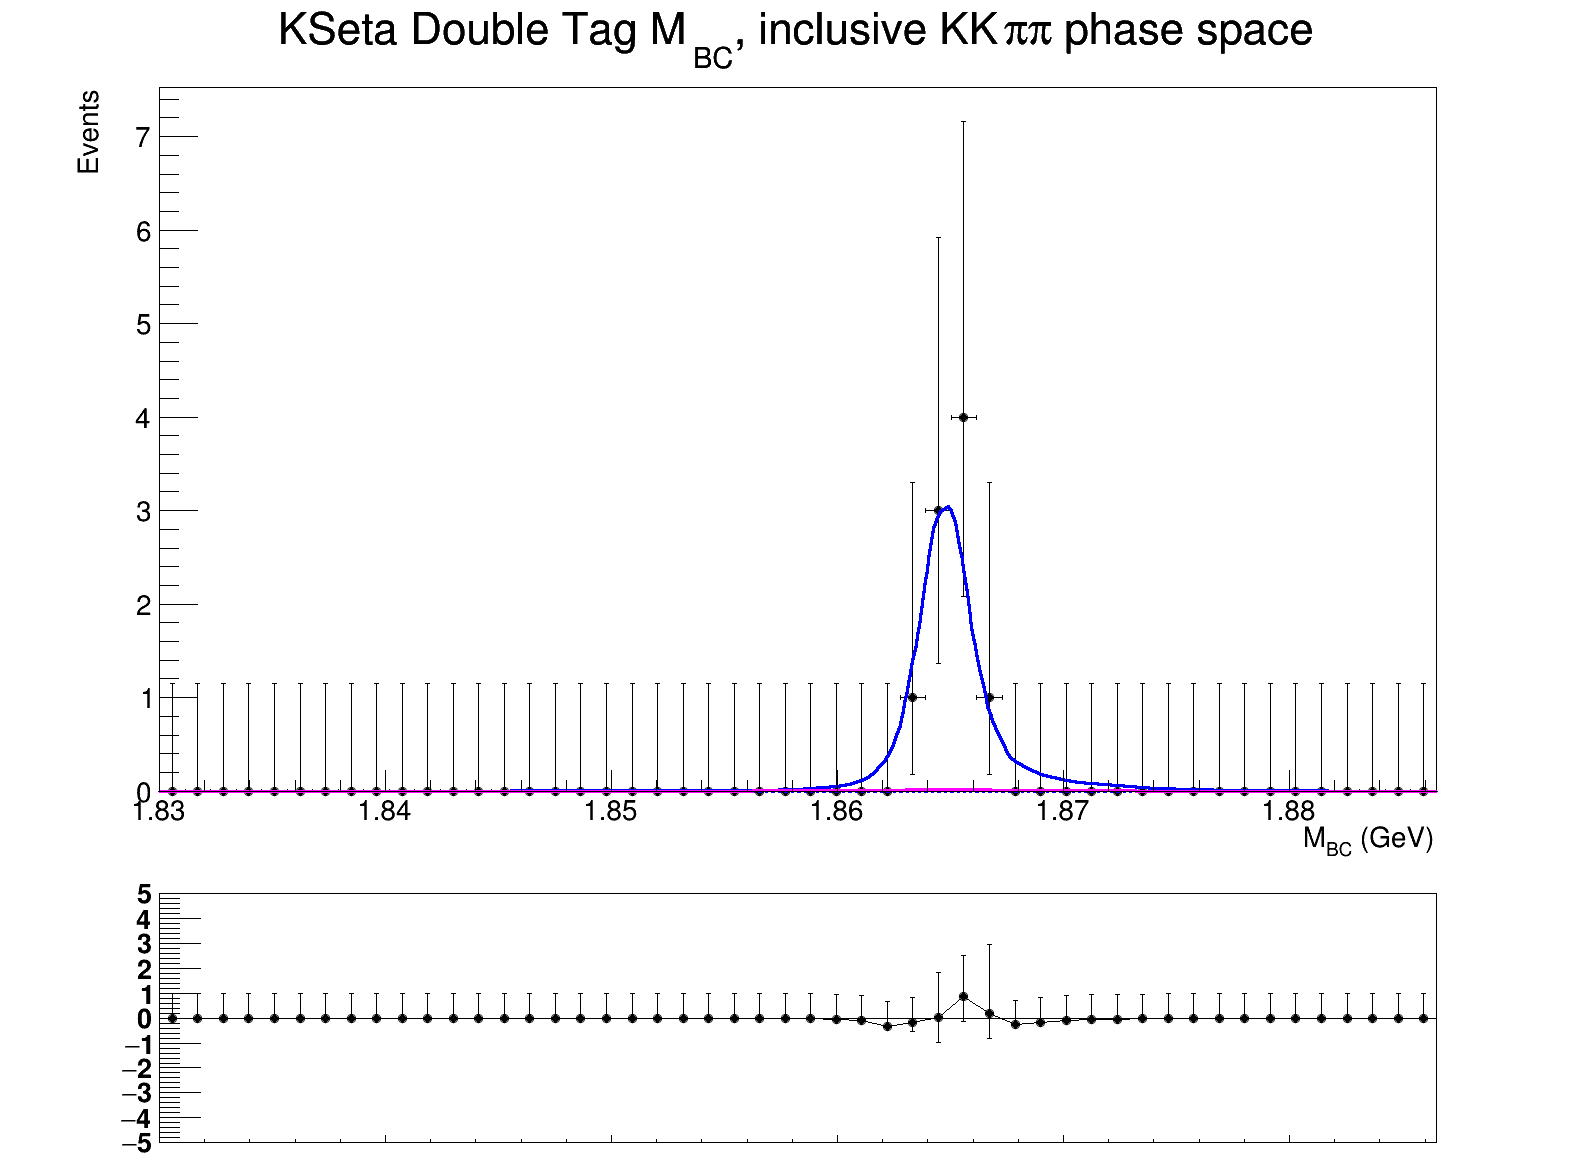
\includegraphics[width=1.0\textwidth]{Plots/DoubleTagYield_DoubleTag_CP_KKpipi_vs_KSeta_SignalBin0.png}
      \caption{$K_S\eta$}
    \end{subfigure}
    \begin{subfigure}{0.33\textwidth}
      \centering
      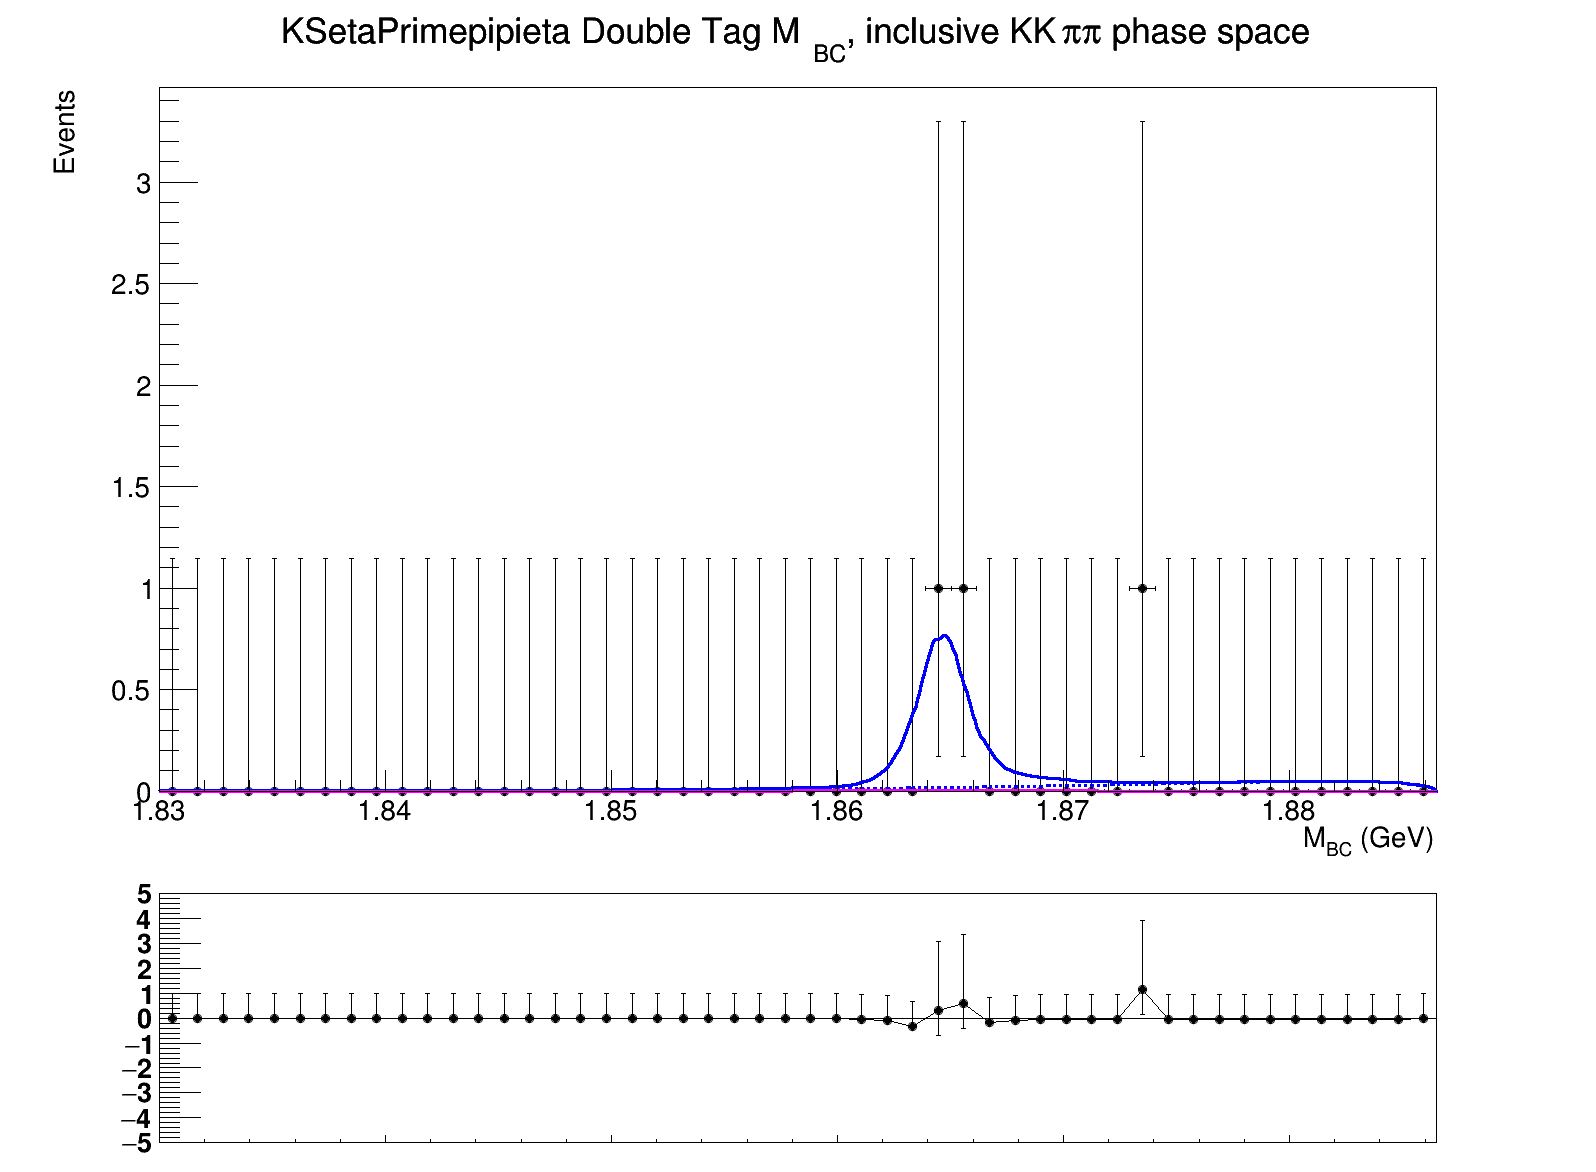
\includegraphics[width=1.0\textwidth]{Plots/DoubleTagYield_DoubleTag_CP_KKpipi_vs_KSetaPrimepipieta_SignalBin0.png}
      \caption{$K_S\eta^\prime(\pi\pi\eta)$}
    \end{subfigure}%
    \begin{subfigure}{0.33\textwidth}
      \centering
      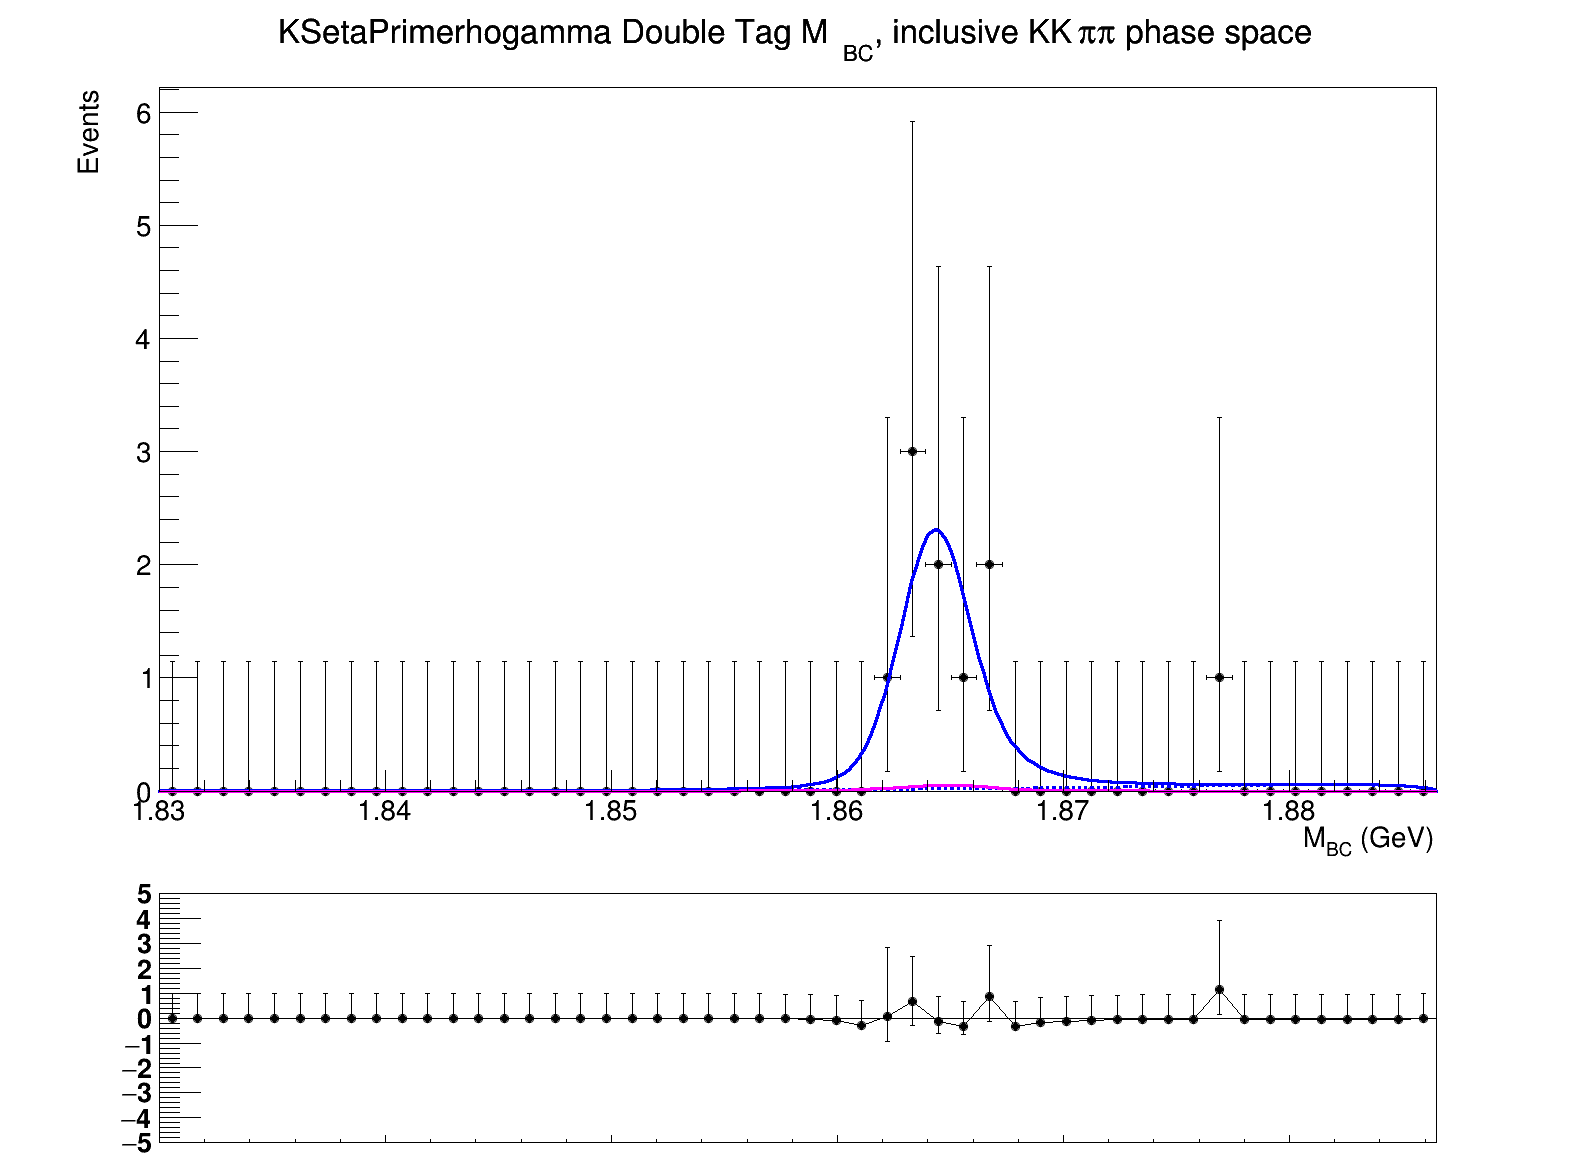
\includegraphics[width=1.0\textwidth]{Plots/DoubleTagYield_DoubleTag_CP_KKpipi_vs_KSetaPrimerhogamma_SignalBin0.png}
      \caption{$K_S\eta^\prime(\rho\gamma)$}
    \end{subfigure}%
    \begin{subfigure}{0.33\textwidth}
      \centering
      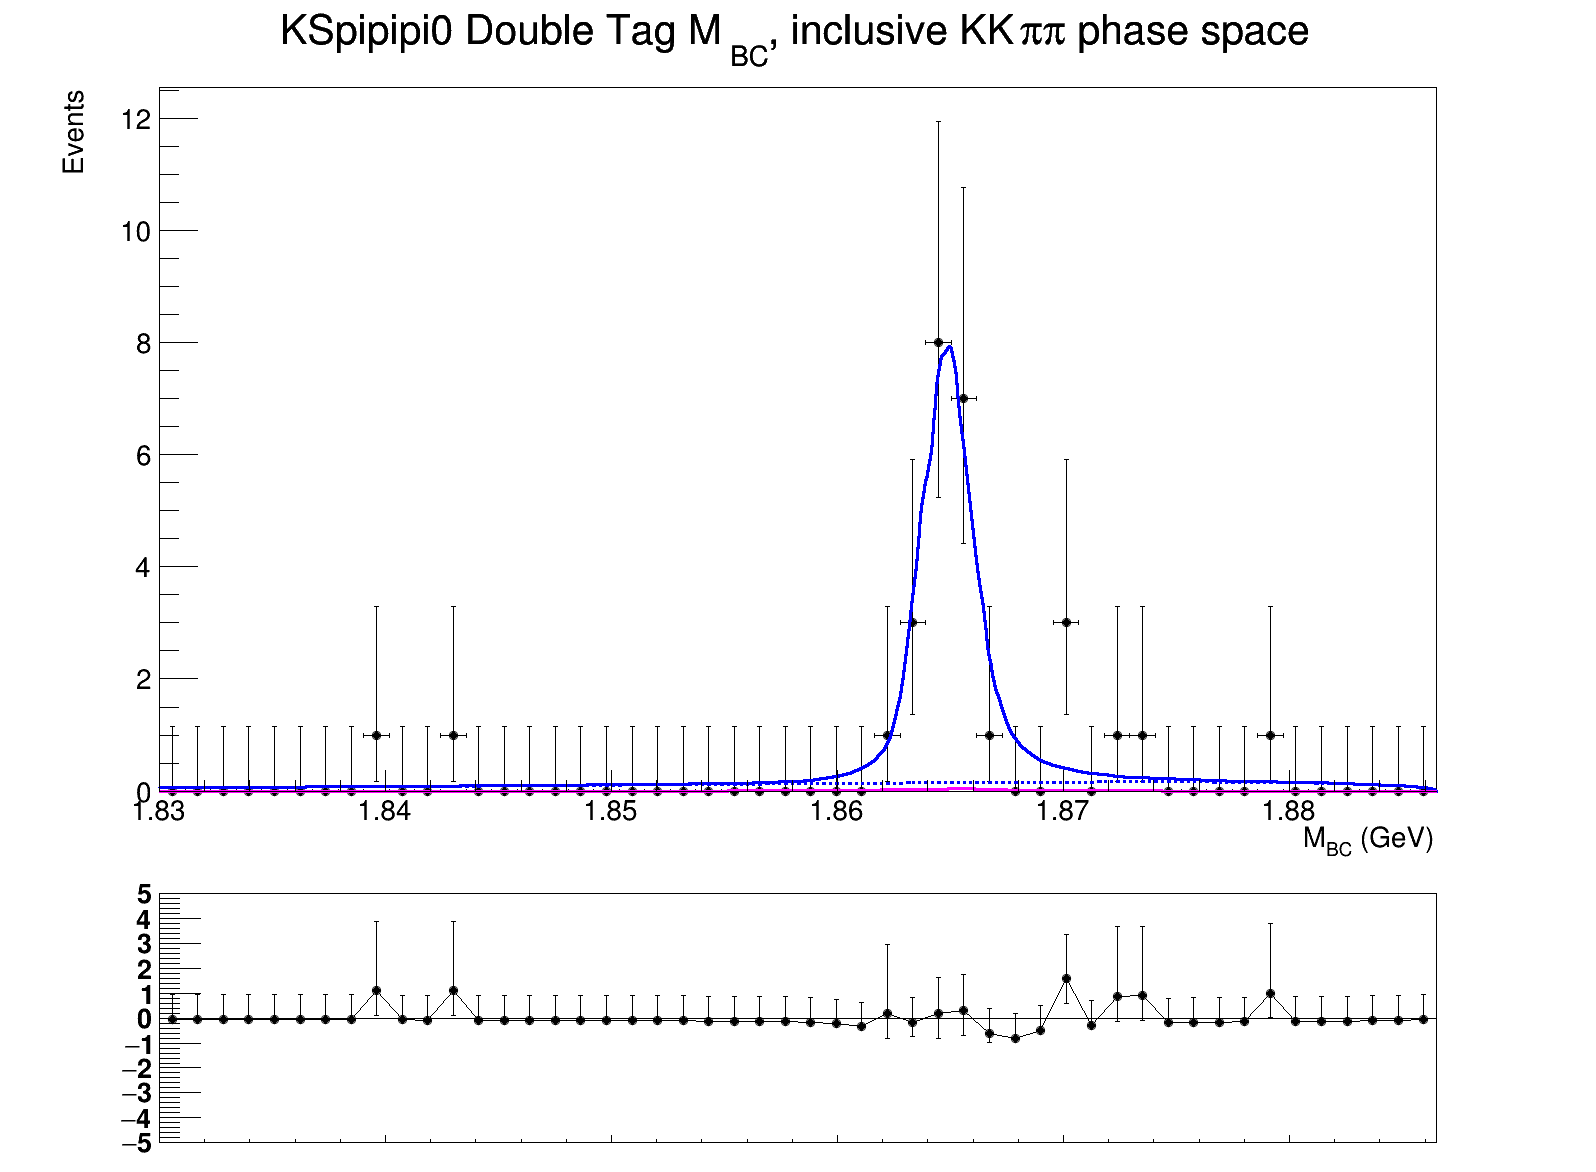
\includegraphics[width=1.0\textwidth]{Plots/DoubleTagYield_DoubleTag_CP_KKpipi_vs_KSpipipi0_SignalBin0.png}
      \caption{$K_S\omega$}
    \end{subfigure}
    \caption{Double tag fits of CP odd tags}
  \end{figure}
\end{frame}

\begin{frame}{CP double tag yields and efficiencies}
  \begin{center}
    \begin{tabular}{lcc}
      \hline
      Tag mode                          & Double tag yield     & Double tag efficiency ($\%$) \\
      \hline
      $K^+K^-$                          & $28 \pm 10$          & $14.52 \pm 0.06$     \\
      $\pi^+\pi^-$                      & $2 \pm 4$            & $15.02 \pm 0.06$     \\
      $K_S\pi^0$                        & $48 \pm 7$           & $6.87 \pm 0.04$      \\
      $K_S\pi^0\pi^0$                   & $8.0 \pm 2.8$        & $2.873 \pm 0.026$    \\
      $K_L\pi^0$                        & $7 \pm 5$            & $5.29 \pm 0.04$      \\
      \hline
      $K_S\eta$                         & $8.9 \pm 3.0$        & $5.72 \pm 0.04$      \\
      $K_S\eta^\prime_{\pi\pi\eta}$     & $2.2 \pm 1.6$        & $2.024 \pm 0.021$    \\
      $K_S\eta^\prime_{\rho\gamma}$     & $8.7 \pm 3.0$        & $3.295 \pm 0.027$    \\
      $\pi^+\pi^-\pi^0$                 & $53 \pm 10$          & $7.66 \pm 0.04$      \\
      $K_S\omega$                       & $9 \pm 3$            & $2.234 \pm 0.022$    \\
      \hline
    \end{tabular}
  \end{center}
\end{frame}

\begin{frame}{Non-resonant background in $K_S\omega$}
  \begin{itemize}
    \setlength\itemsep{0.5em}
    \item{$K_S\omega$ has CP-even contamination from non-resonant $K_S\pi\pi\pi^0$}
    \begin{itemize}
      \item{$F_+(K_S\pi\pi\pi^0) = 0.238\pm0.012\pm0.012$ from CLEO}
    \end{itemize}
    \item{From $m_{\rm BC}$ fit, subtract flat background using sPlot and fit $\pi\pi\pi^0$}
  \end{itemize}
  \begin{figure}
    \centering
    \begin{subfigure}{0.5\textwidth}
      \centering
      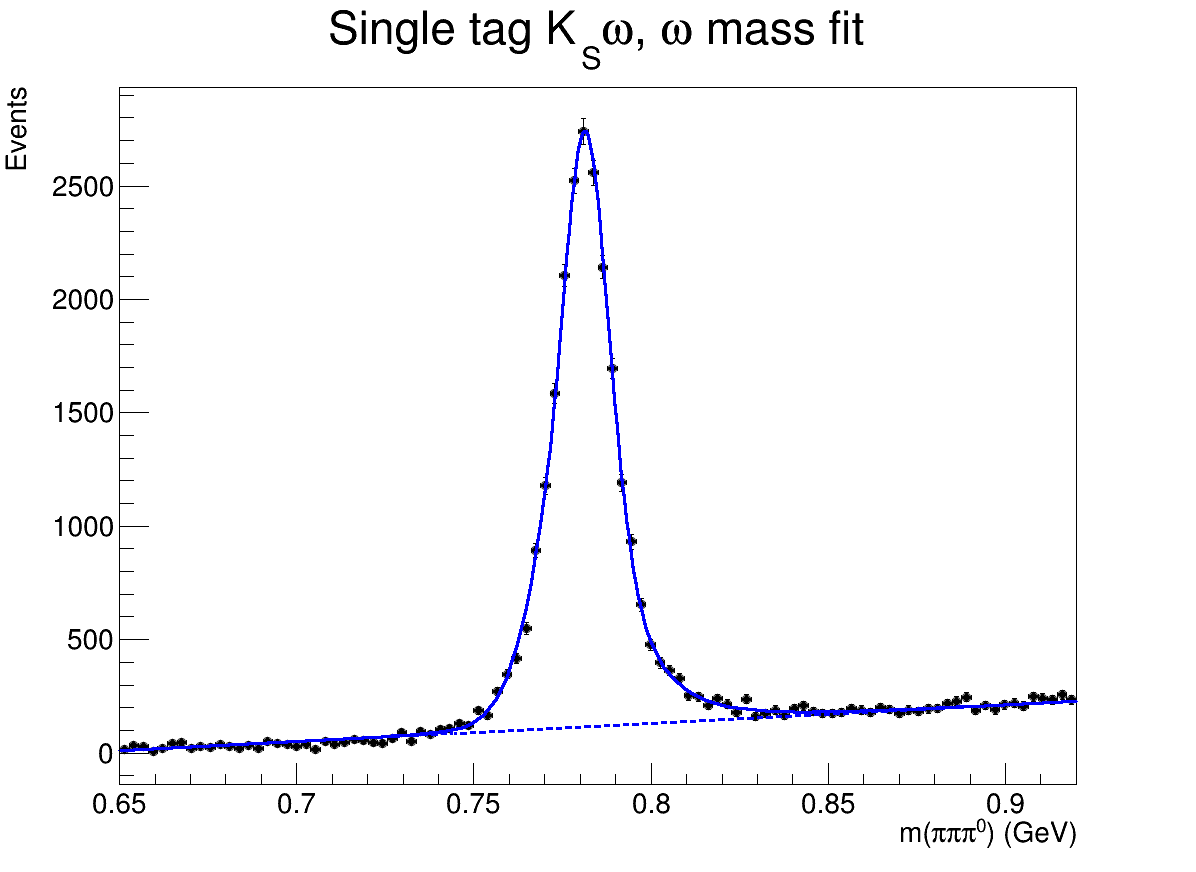
\includegraphics[width=1.0\textwidth]{Plots/KSomega_ST_Mpipipi0.png}
      \caption{Single tag}
    \end{subfigure}%
    \begin{subfigure}{0.5\textwidth}
      \centering
      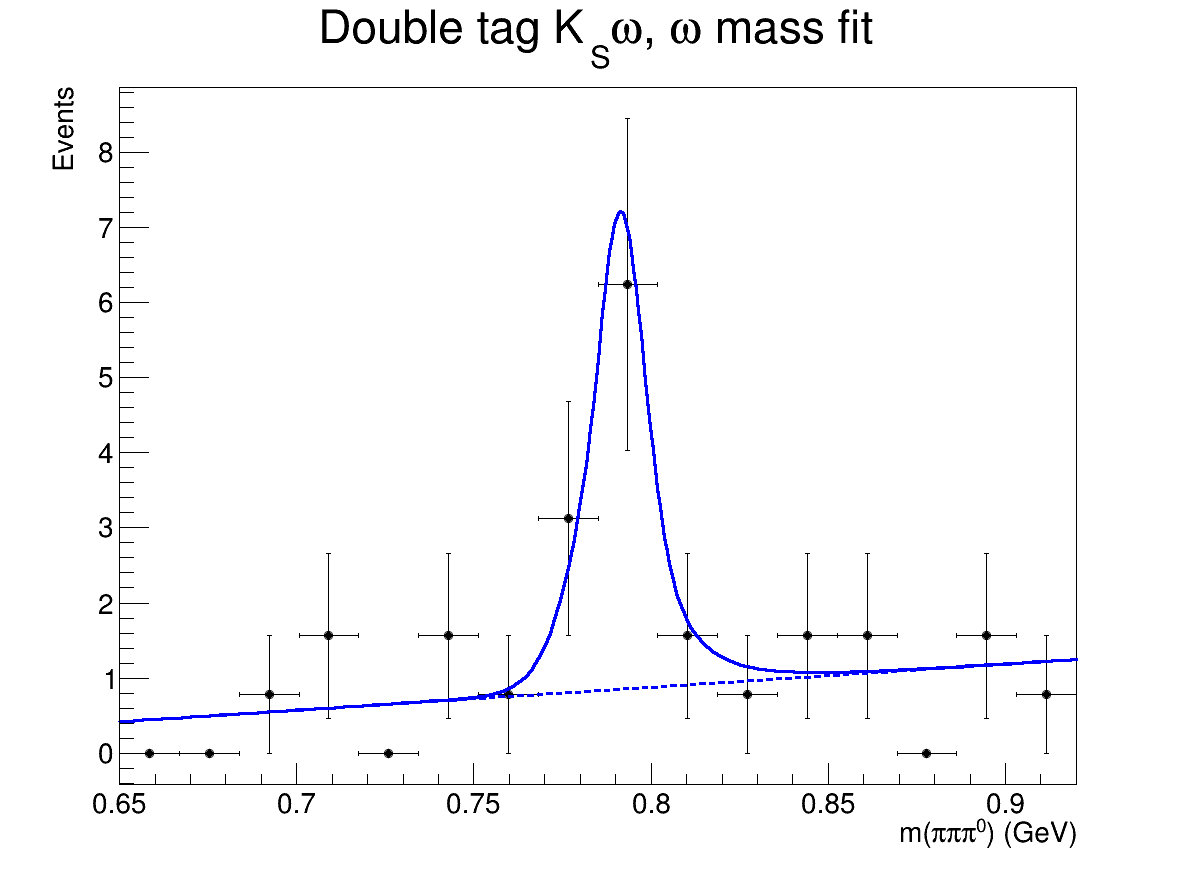
\includegraphics[width=1.0\textwidth]{Plots/KSomega_DT_Mpipipi0.png}
      \caption{Double tag}
    \end{subfigure}
  \end{figure}
\end{frame}

\subsection{\texorpdfstring{$K_{S, L}\pi\pi$}{K0pipi} tags}

\begin{frame}{$F_+$ measurement with $K_{S, L}\pi\pi$ tags}
  \begin{itemize}
    \item{With $K_S\pi\pi$, increase sensitivity through binning of $K_S\pi\pi$ phase space}
  \end{itemize}
  \begin{center}
    $M_j\propto\big(K^\prime_j + K^\prime_{-j} - 2\sqrt{K^\prime_jK^\prime_{-j}}c^\prime_j(2F_+^{KK\pi\pi} - 1)\big)$
  \end{center}
  \begin{itemize}
    \item{Problem: $KK\pi\pi$ reconstruction efficiency is too low $\to$ Low yields!}
  \end{itemize}
  \begin{figure}
    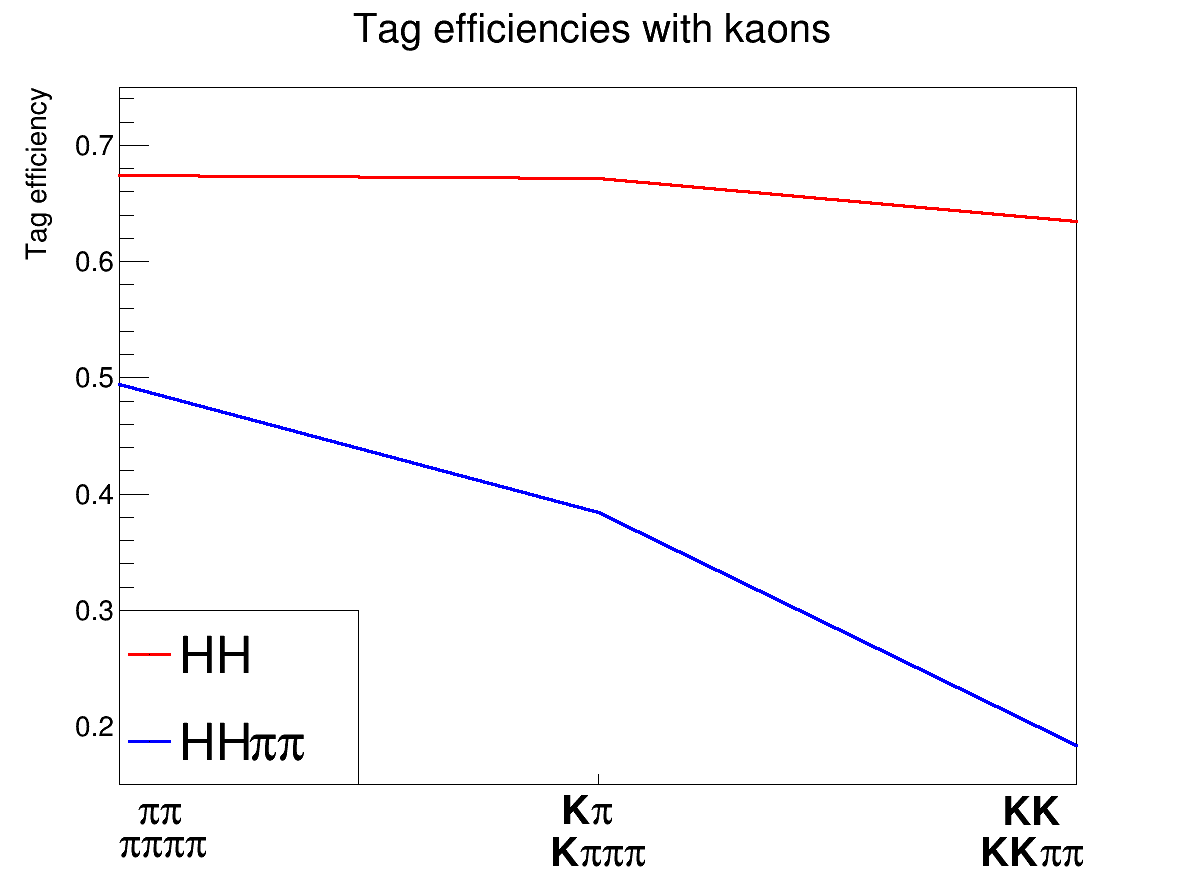
\includegraphics[width = 0.5\textwidth]{Plots/KaonTrackingEfficiency.png}
  \end{figure}
  \begin{itemize}
    \item{Likely explanation: Softer kaons $\to$ Kaons get stuck inside tracker}
  \end{itemize}
\end{frame}

\begin{frame}{$F_+$ measurement with $K_{S, L}\pi\pi$ tags}
  \begin{itemize}
    \setlength\itemsep{1.0em}
    \item{Solution: Partially reconstructed $KK\pi\pi$}
    \item{Strategy:}
    \begin{enumerate}
      \setlength\itemsep{0.5em}
      \item{Reconstruct $D\to K_S\pi\pi$}
      \item{Require 3 remaining good tracks consistent with $K\pi\pi$}
      \item{Use missing mass to reconstruct missing kaon}
    \end{enumerate}
  \end{itemize}
  \vspace{0.5cm}
  \def\arraystretch{1.2}%
  \begin{tabular}{lcc}
    Mode                                     & Inclusive yield  & Double tag efficiency \\
    \hline
    $K_S\pi\pi$ (fully reconstructed)        & $\SI{69(9)}{}$   & $\SI{6.56(4)}{}$ \\
    $K_S\pi\pi$ (partially reconstructed)    & $\SI{91(15)}{}$  & $\SI{7.01(4)}{}$ \\
    $K_L\pi\pi$ (partially reconstructed)    & $\SI{158(15)}{}$ & $\SI{7.25(4)}{}$ \\
    \hline
  \end{tabular}
\end{frame}

\begin{frame}{Partially reconstructed $KK\pi\pi$ vs $K_S\pi\pi$}
  \begin{itemize}
    \item{Main challenge with partially reconstructed $KK\pi\pi$: $K\pi\pi\pi\pi^0$}
    \item{Require no $\pi^0$ candidates}
  \end{itemize}
  \begin{figure}
    \centering
    \vspace{-0.2cm}
    \begin{subfigure}{0.50\textwidth}
      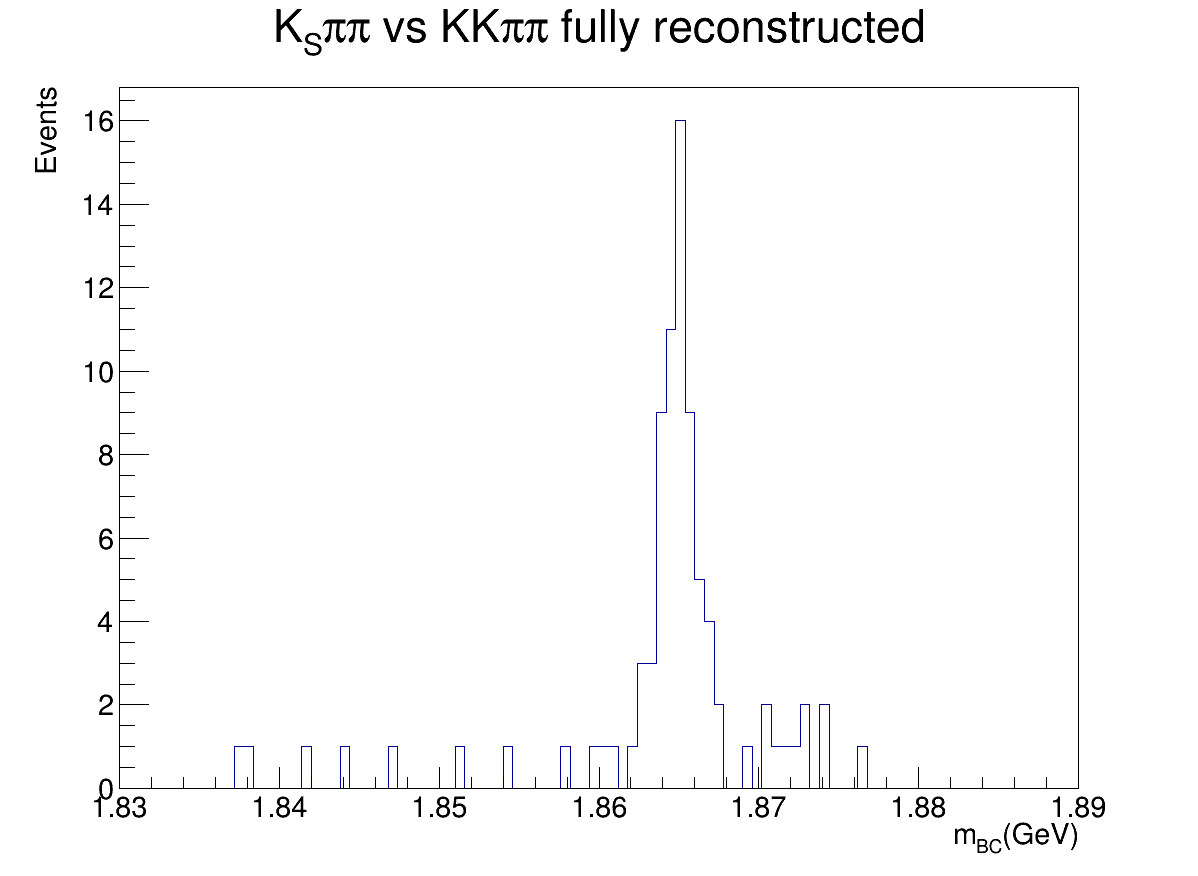
\includegraphics[width = 1.0\textwidth]{Plots/KKpipiVersusKSpipiMBC.png}
      \caption{Fully reconstructed}
    \end{subfigure}%
    \begin{subfigure}{0.50\textwidth}
      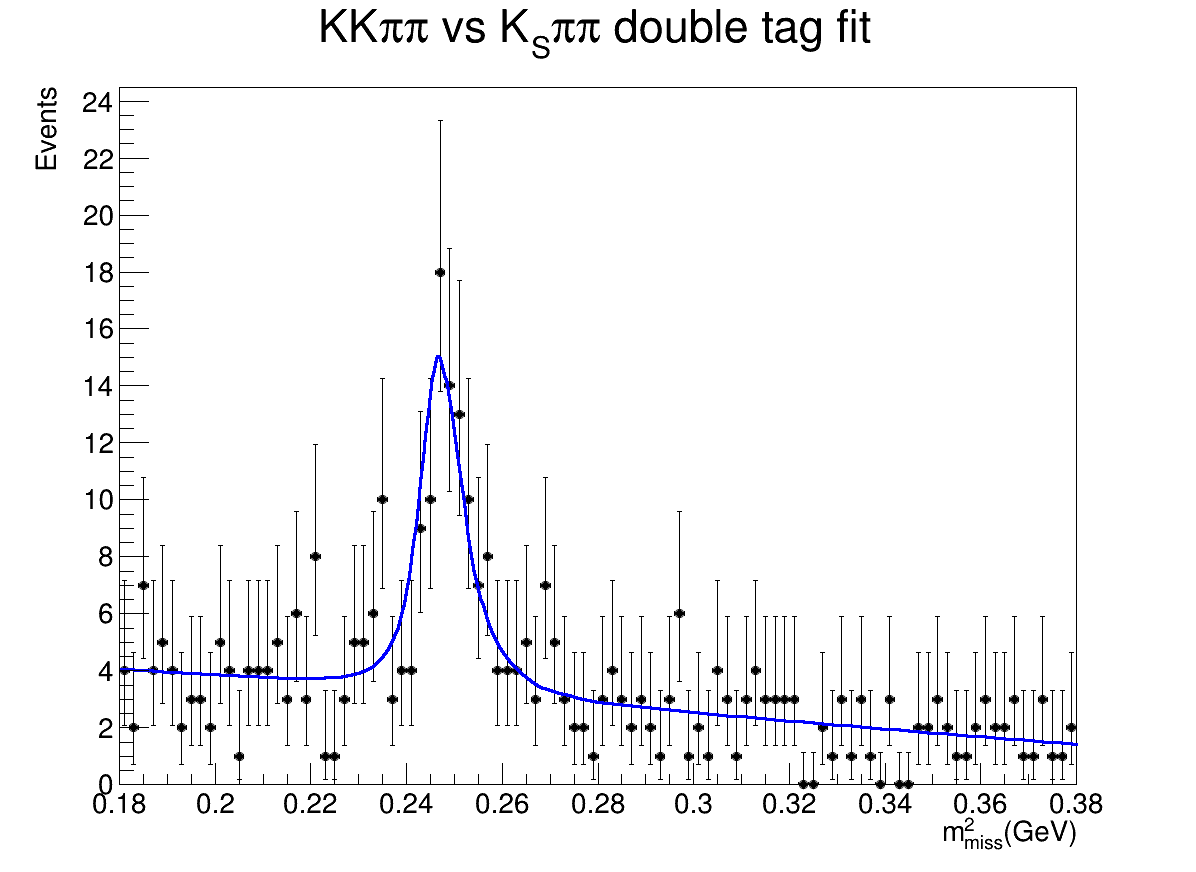
\includegraphics[width = 1.0\textwidth]{Plots/KSpipiPartReco_Inclusive_DoubleTagYield.png}
      \caption{Partially reconstructed}
    \end{subfigure}
    \caption{$KK\pi\pi$ vs $K_S\pi\pi$}
  \end{figure}
\end{frame}

\begin{frame}{Double tag fits}
  \begin{figure}
    \centering
    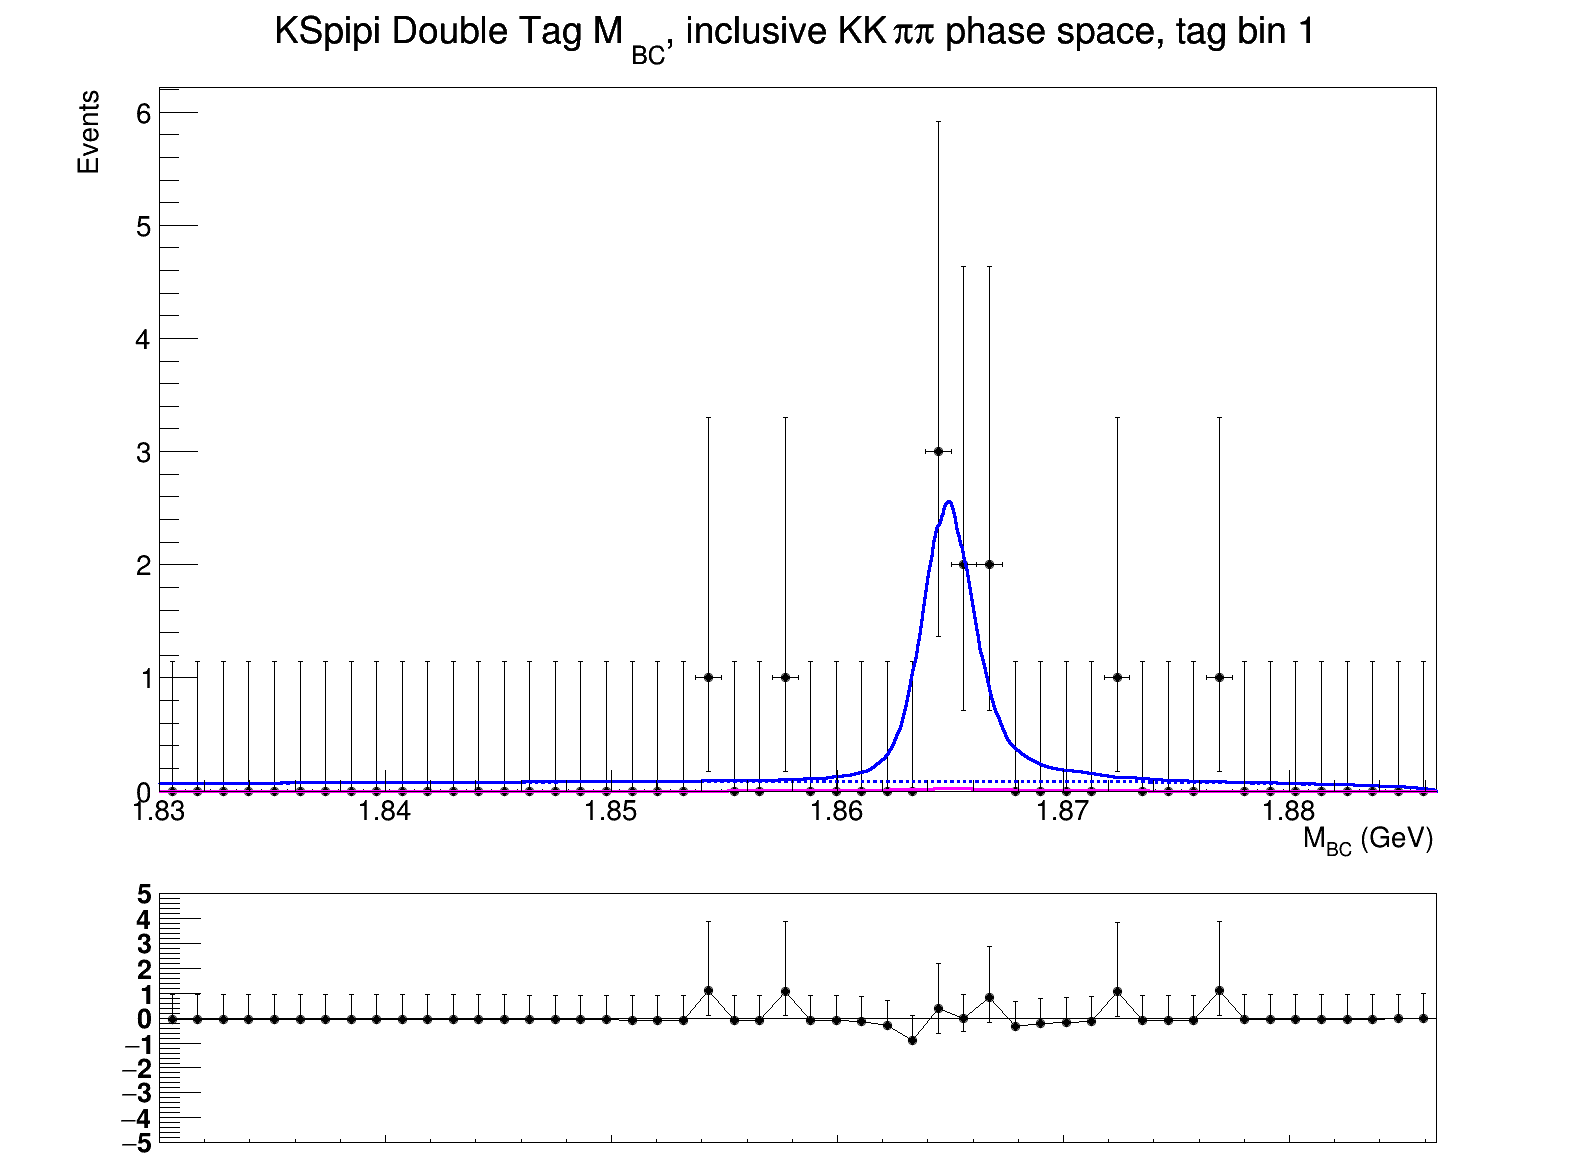
\includegraphics[width=0.32\textwidth, clip = true, trim = {0 11cm 0 0}]{Plots/DoubleTagYield_DoubleTag_SCMB_KKpipi_vs_KSpipi_SignalBin0_TagBin1.png}
    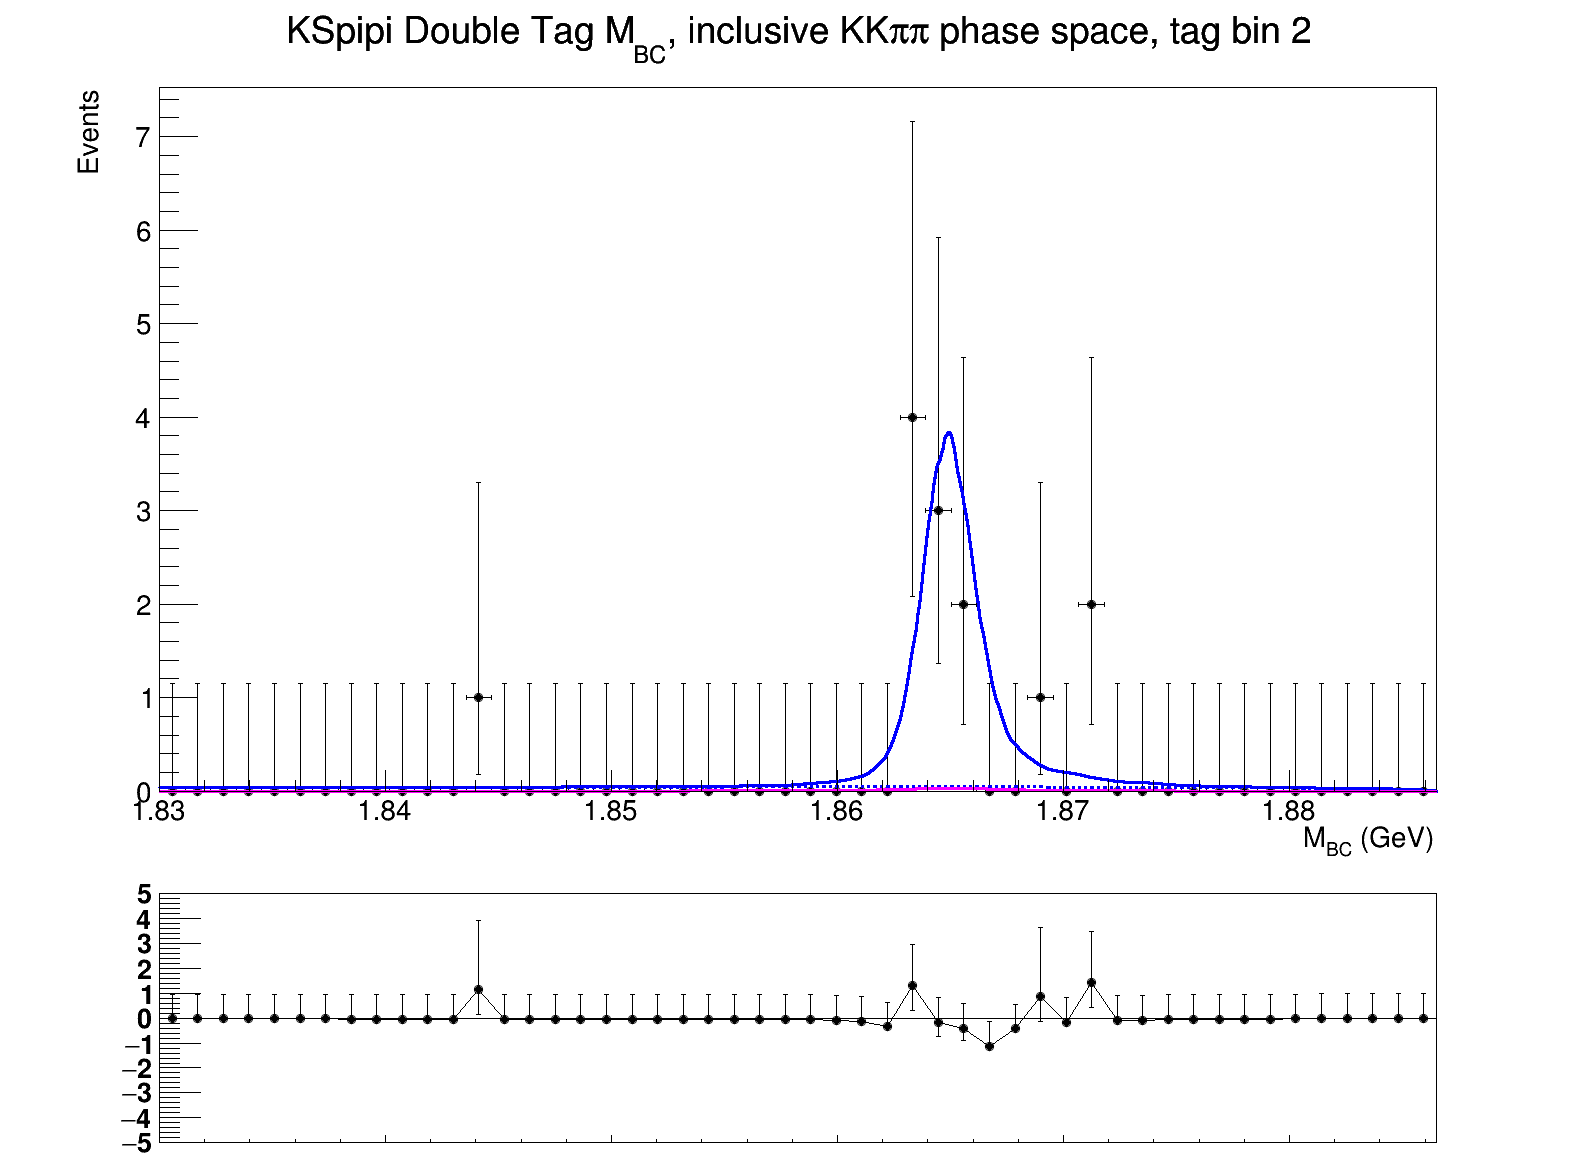
\includegraphics[width=0.32\textwidth, clip = true, trim = {0 11cm 0 0}]{Plots/DoubleTagYield_DoubleTag_SCMB_KKpipi_vs_KSpipi_SignalBin0_TagBin2.png}
    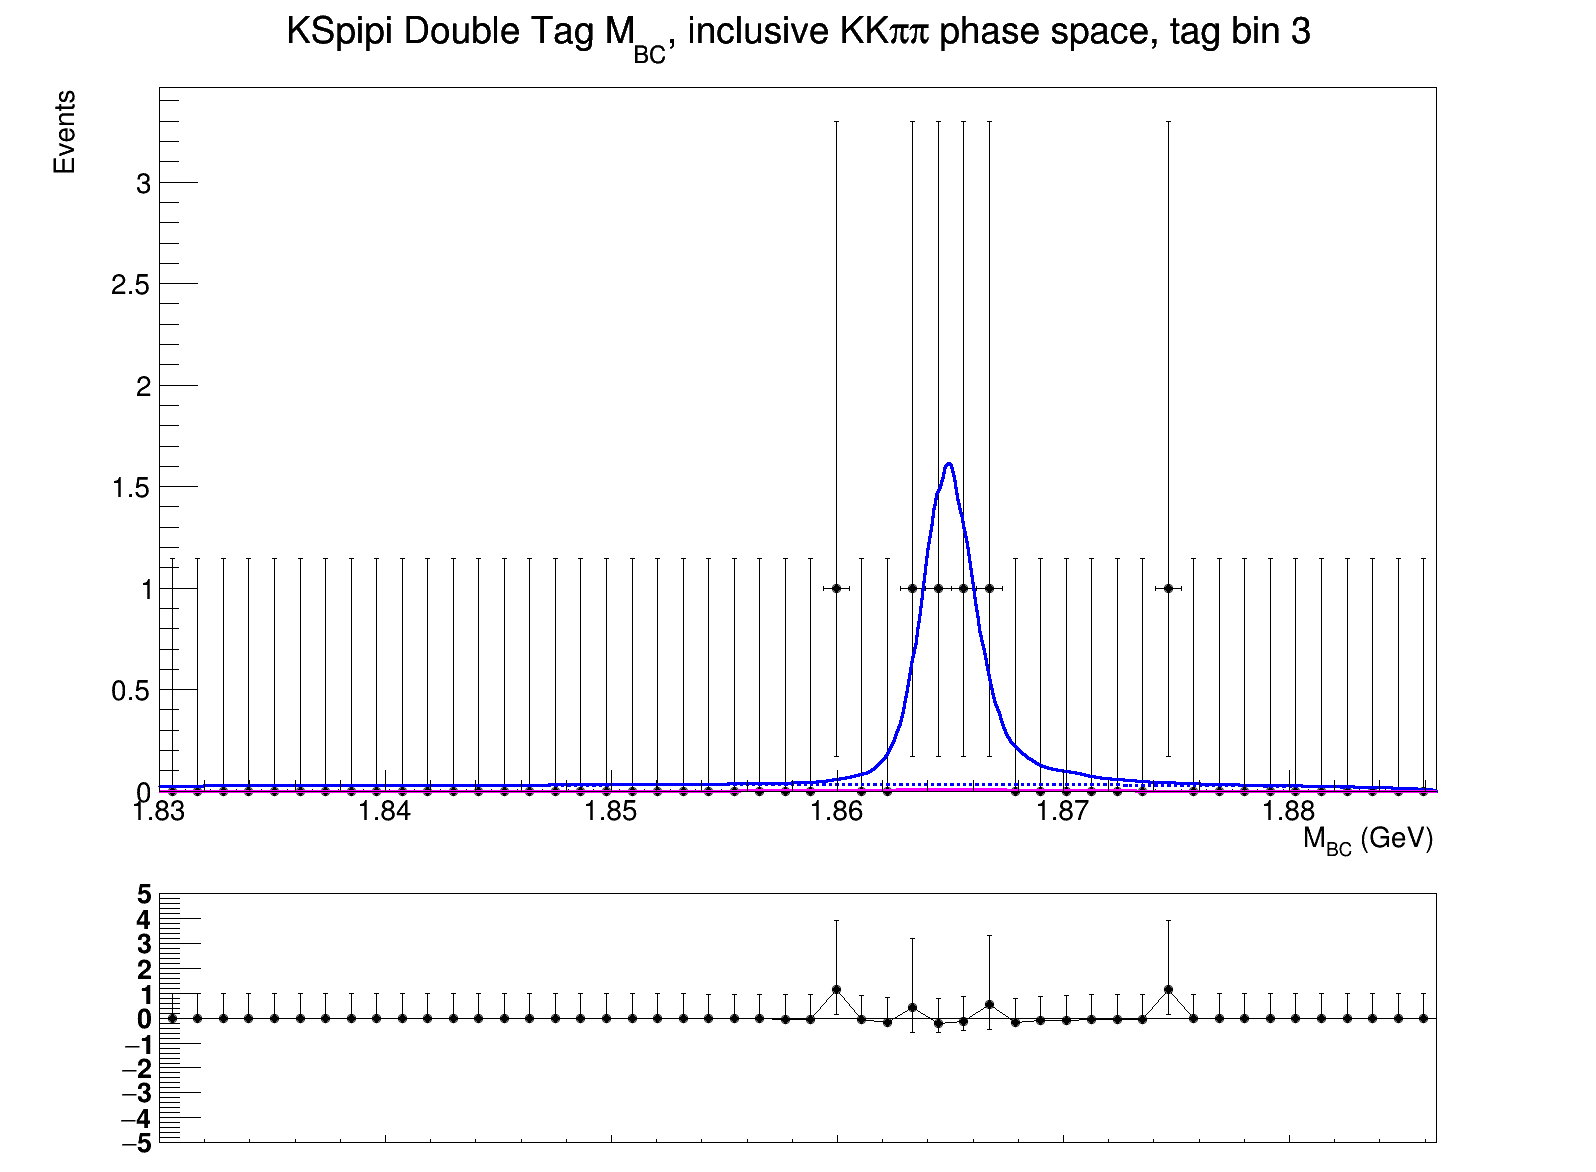
\includegraphics[width=0.32\textwidth, clip = true, trim = {0 11cm 0 0}]{Plots/DoubleTagYield_DoubleTag_SCMB_KKpipi_vs_KSpipi_SignalBin0_TagBin3.png}
    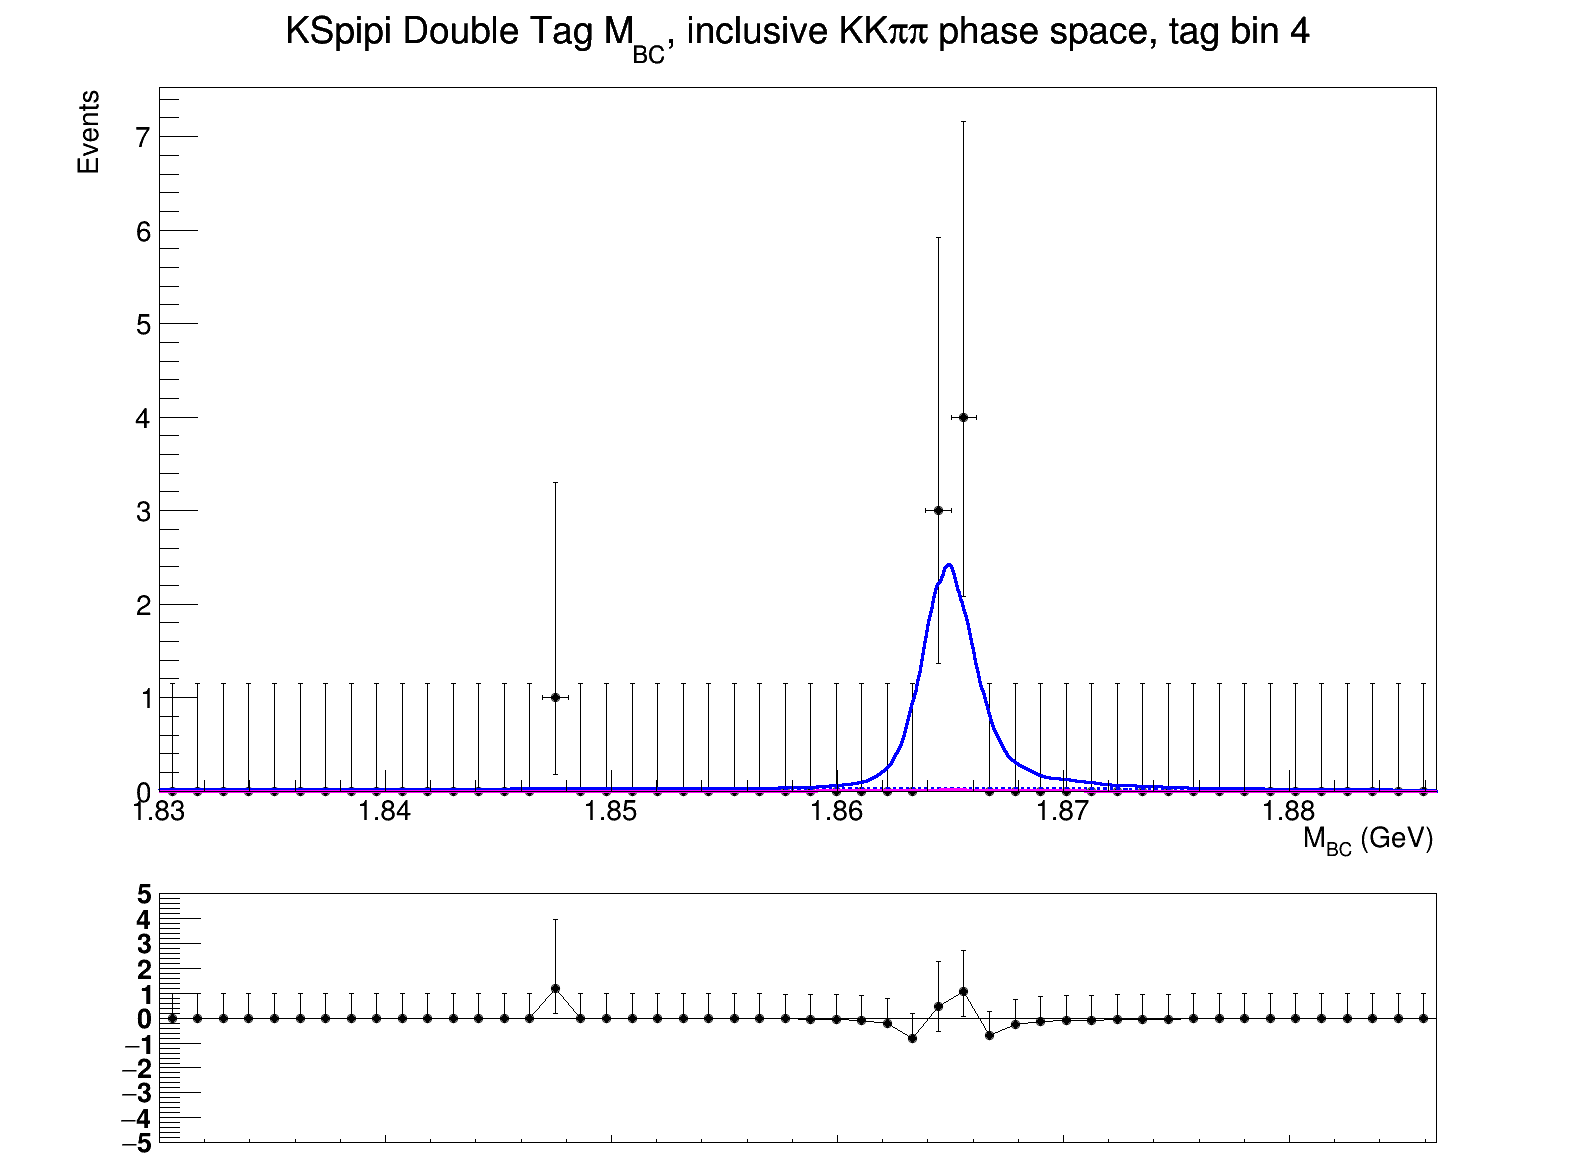
\includegraphics[width=0.32\textwidth, clip = true, trim = {0 11cm 0 0}]{Plots/DoubleTagYield_DoubleTag_SCMB_KKpipi_vs_KSpipi_SignalBin0_TagBin4.png}
    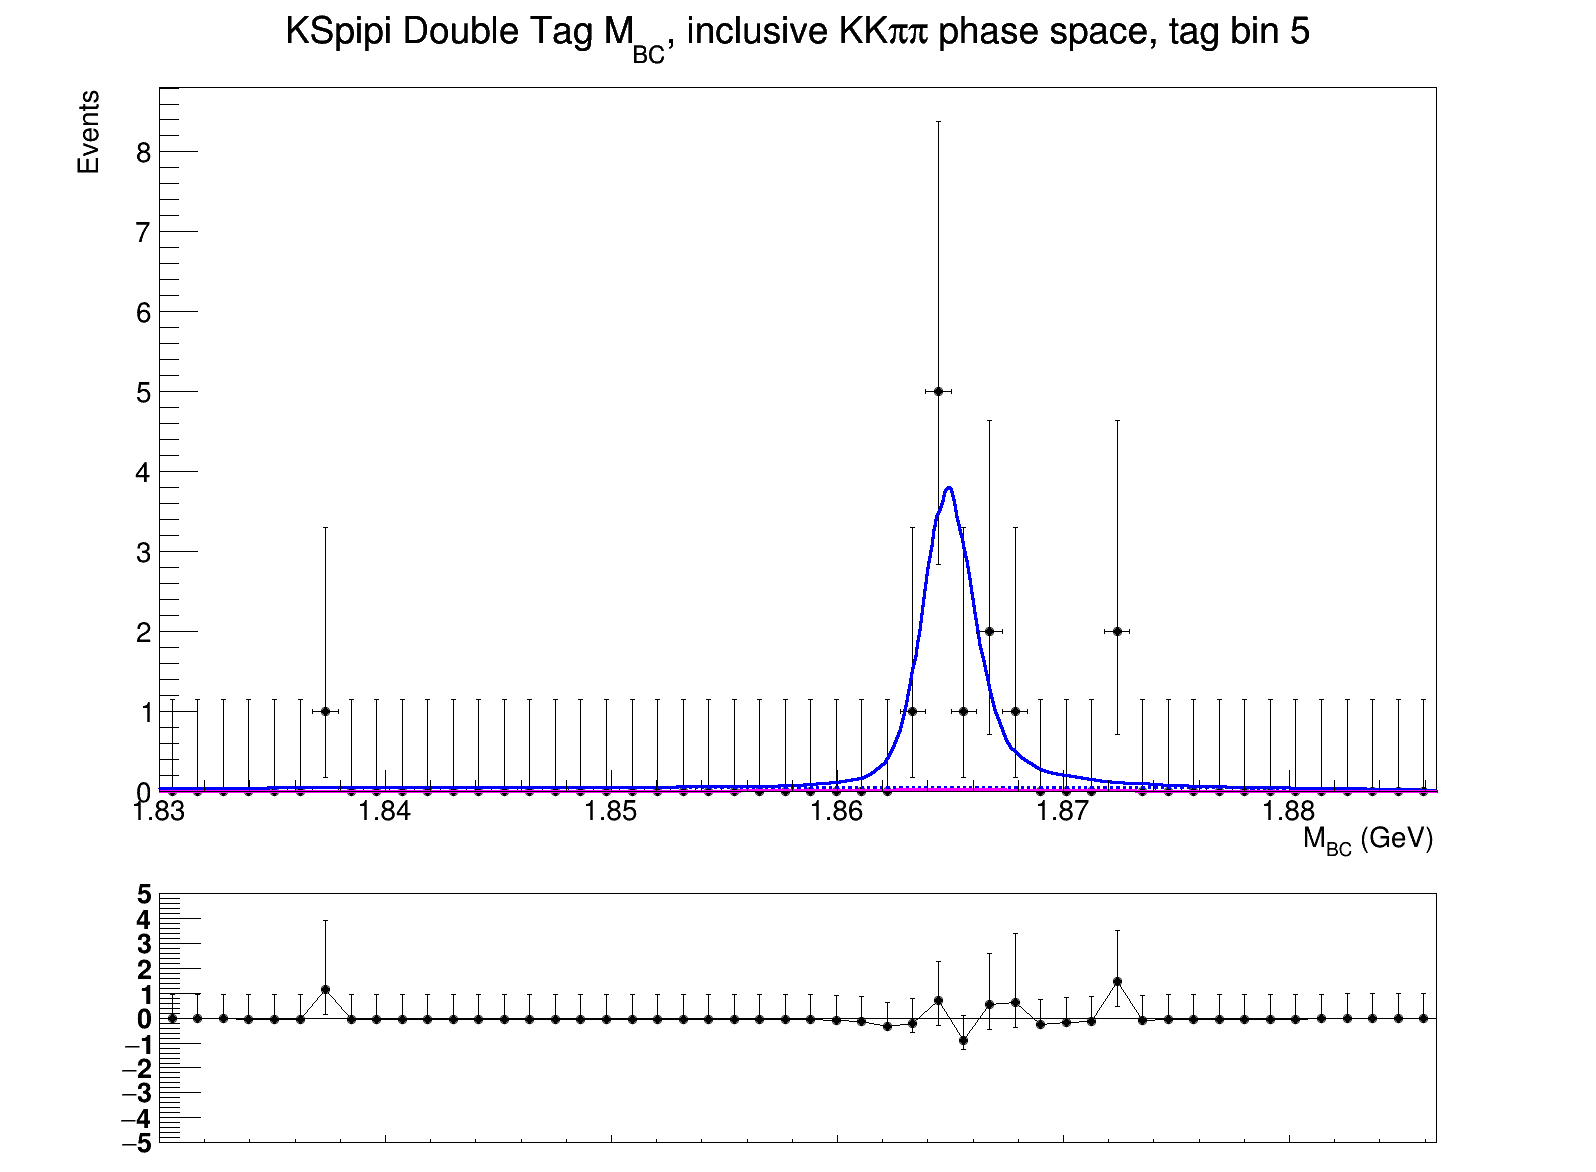
\includegraphics[width=0.32\textwidth, clip = true, trim = {0 11cm 0 0}]{Plots/DoubleTagYield_DoubleTag_SCMB_KKpipi_vs_KSpipi_SignalBin0_TagBin5.png}
    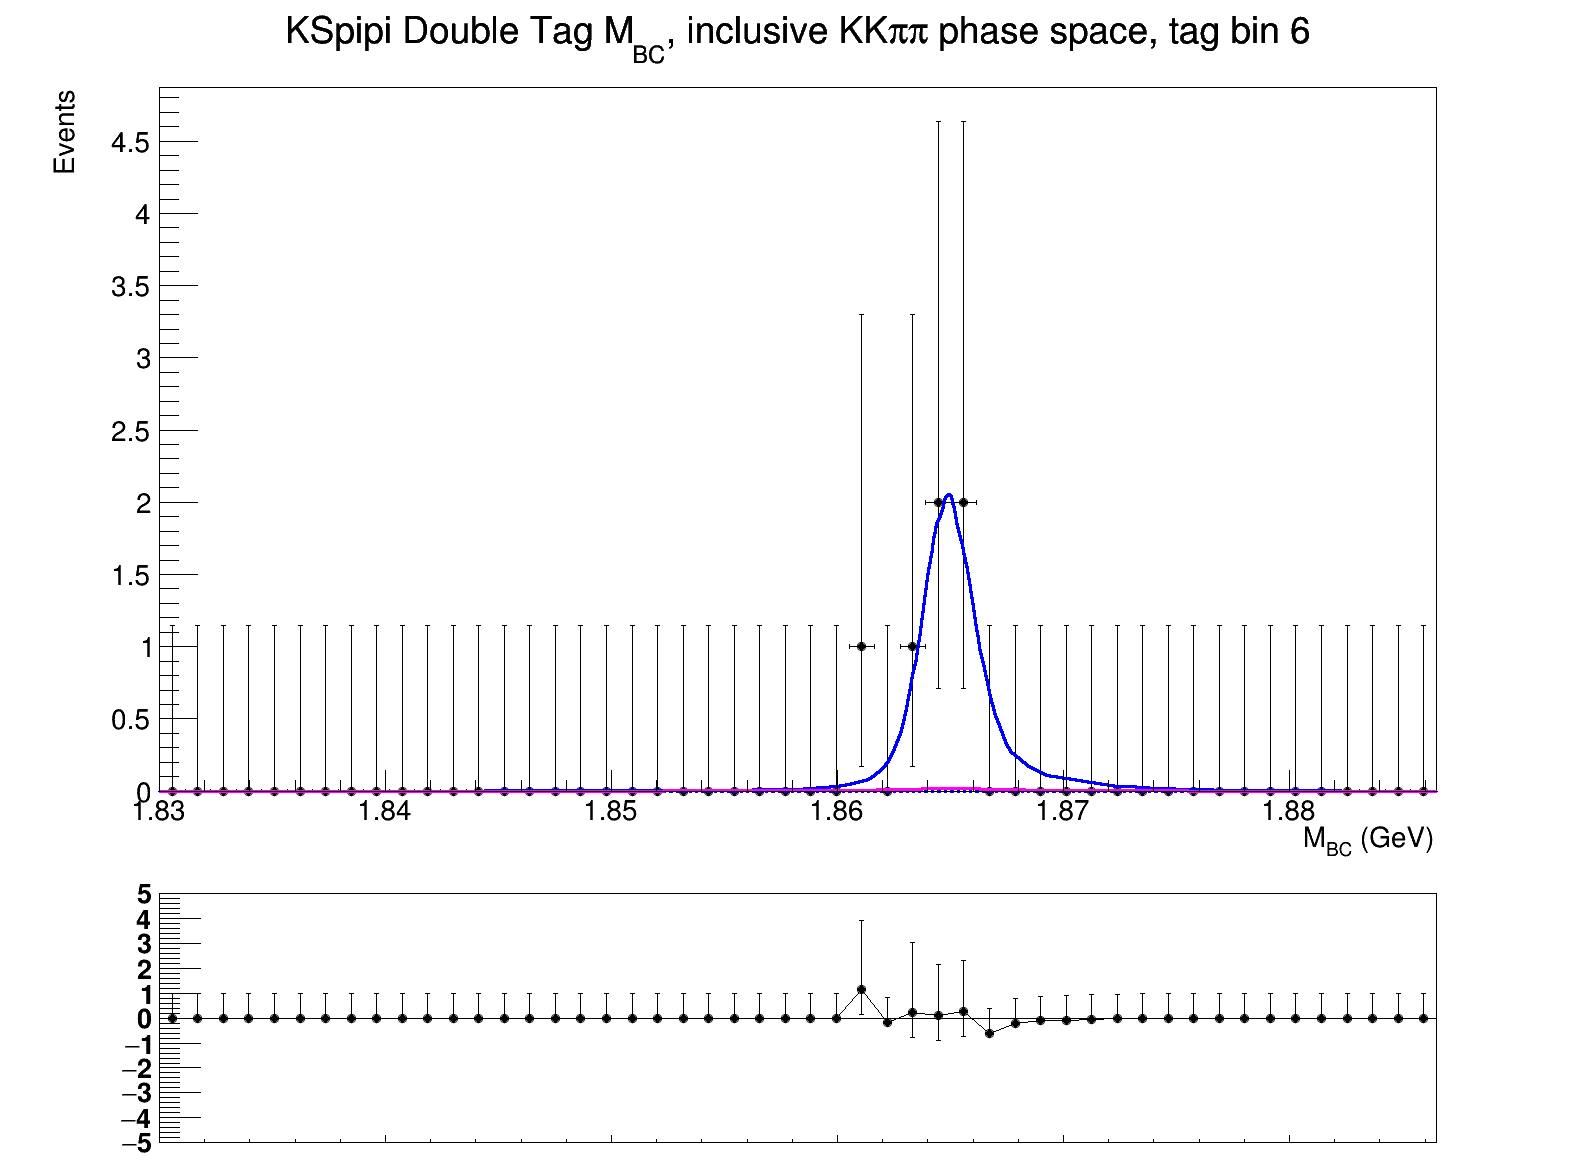
\includegraphics[width=0.32\textwidth, clip = true, trim = {0 11cm 0 0}]{Plots/DoubleTagYield_DoubleTag_SCMB_KKpipi_vs_KSpipi_SignalBin0_TagBin6.png}
    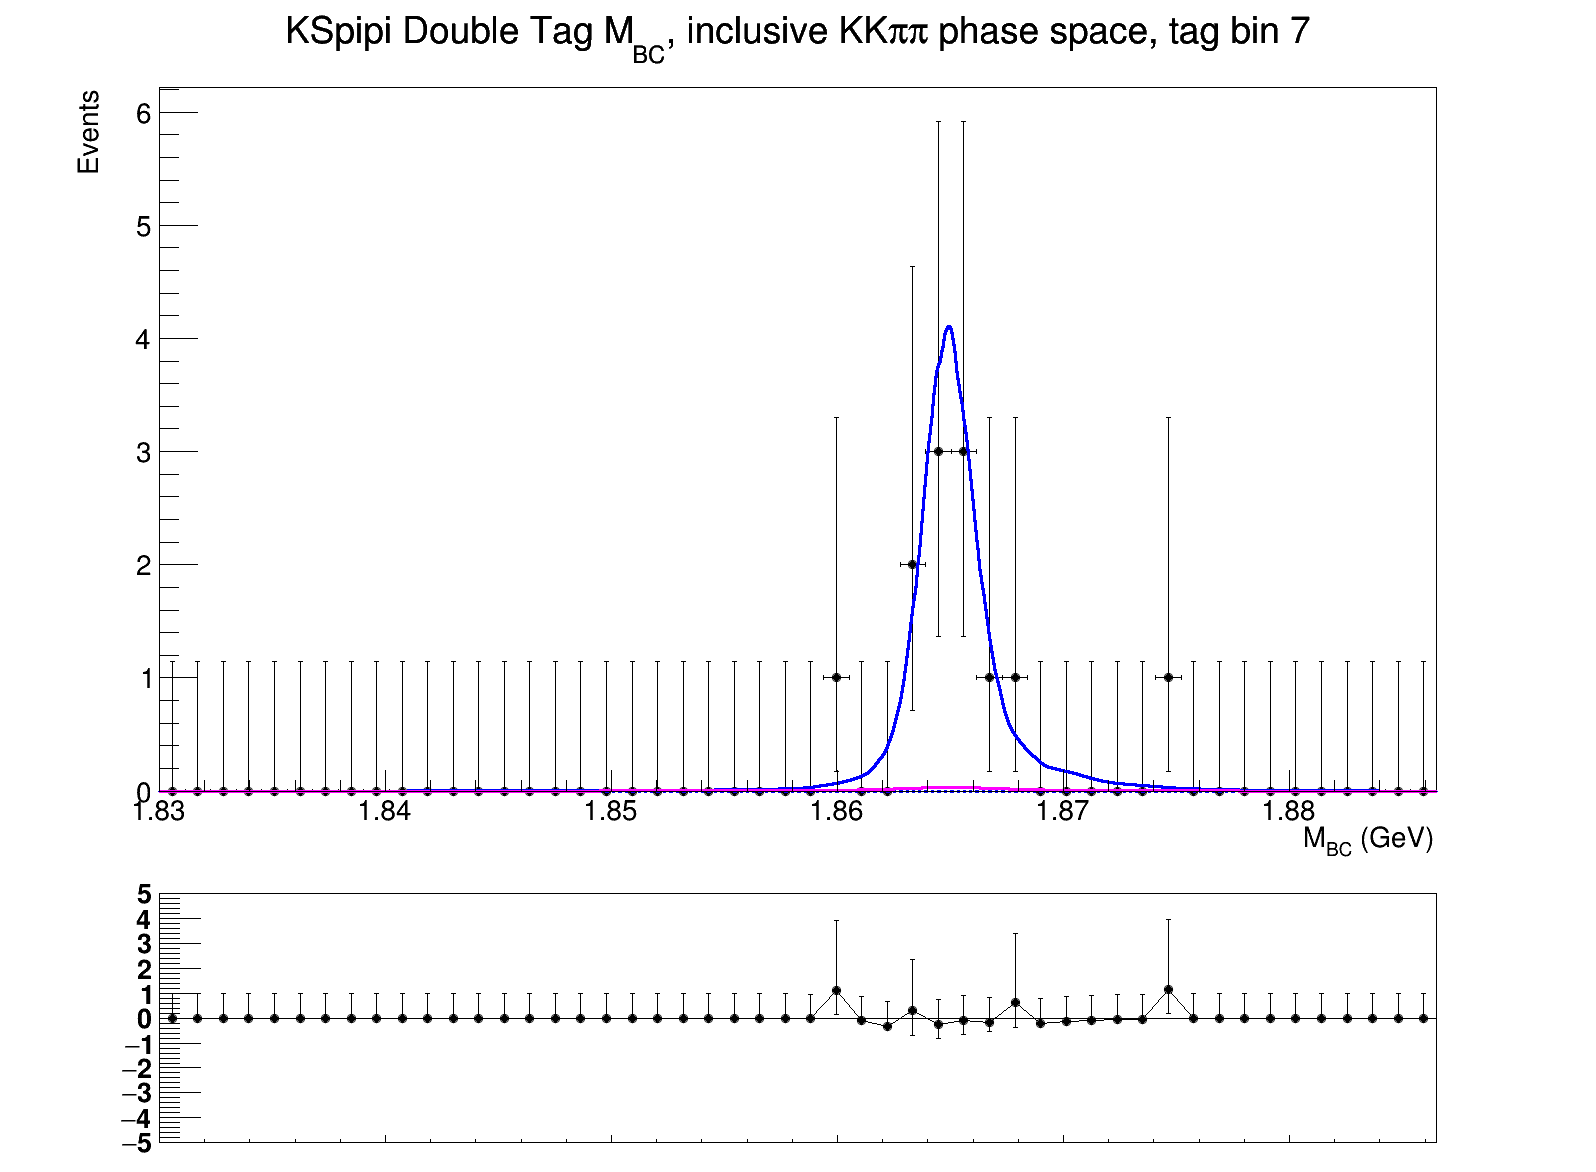
\includegraphics[width=0.32\textwidth, clip = true, trim = {0 11cm 0 0}]{Plots/DoubleTagYield_DoubleTag_SCMB_KKpipi_vs_KSpipi_SignalBin0_TagBin7.png}
    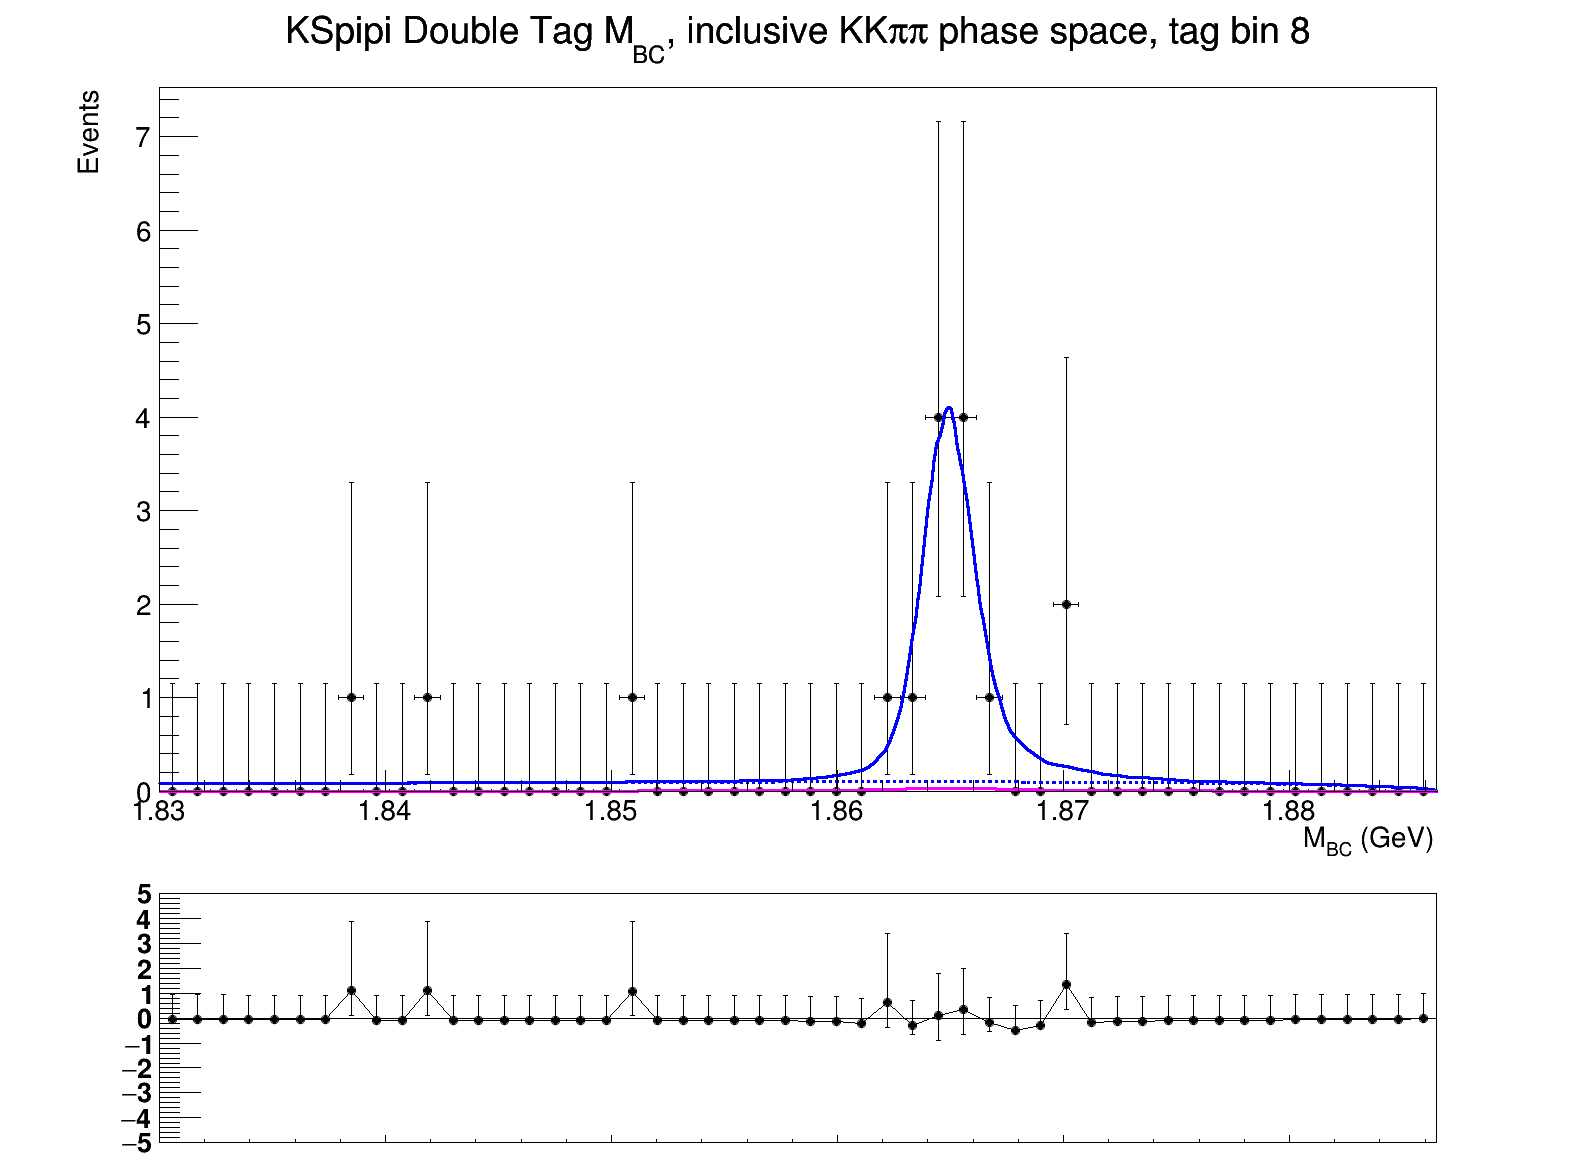
\includegraphics[width=0.32\textwidth, clip = true, trim = {0 11cm 0 0}]{Plots/DoubleTagYield_DoubleTag_SCMB_KKpipi_vs_KSpipi_SignalBin0_TagBin8.png}
    \caption{$KK\pi\pi$ vs $K_S\pi\pi$ simultaneous fit}
  \end{figure}
\end{frame}

\section{Reweighting of \texorpdfstring{$KK\pi\pi$}{KKpipi} model}

\begin{frame}{Efficiency corrections}
  \begin{itemize}
    \setlength\itemsep{1.5em}
    \item{All yields must be corrected for efficiency}
    \item{Problem: BESIII simulation uses a very old $KK\pi\pi$ model in EvtGen}
    \item{Solution: Reweight BESIII simulation to look like the LHCb model}
    \begin{itemize}
      \setlength\itemsep{0.5em}
      \item{Use Python hep\textunderscore ml Gradient Boosted Reweighter}
      \item{Variables:}
      \begin{enumerate}
        \item{$m^2(K^+K^-)$}
        \item{$m^2(K^+\pi^-)$}
        \item{$m^2(K^-\pi^+)$}
        \item{$m^2(\pi^+\pi^-)$}
        \item{$m^2(K^+K^-\pi^+)$}
      \end{enumerate}
    \end{itemize}
  \end{itemize}
\end{frame}

\begin{frame}{Naive efficiency correction}
  \begin{figure}
    \begin{subfigure}{0.33\textwidth}
      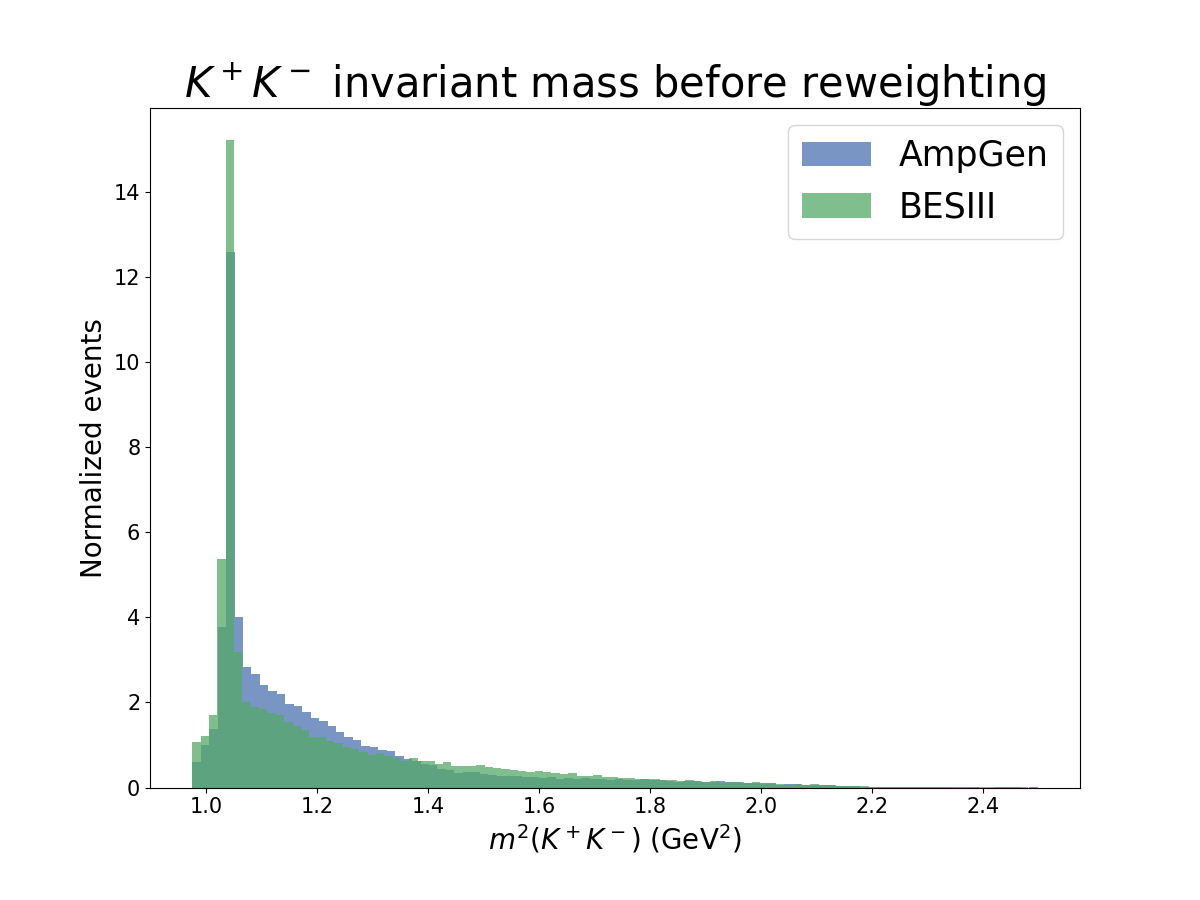
\includegraphics[width = 1.0\textwidth]{Plots/s01_BeforeReweighting.png}
      \caption{$m^2(K^+K^-)$}
    \end{subfigure}%
    \begin{subfigure}{0.33\textwidth}
      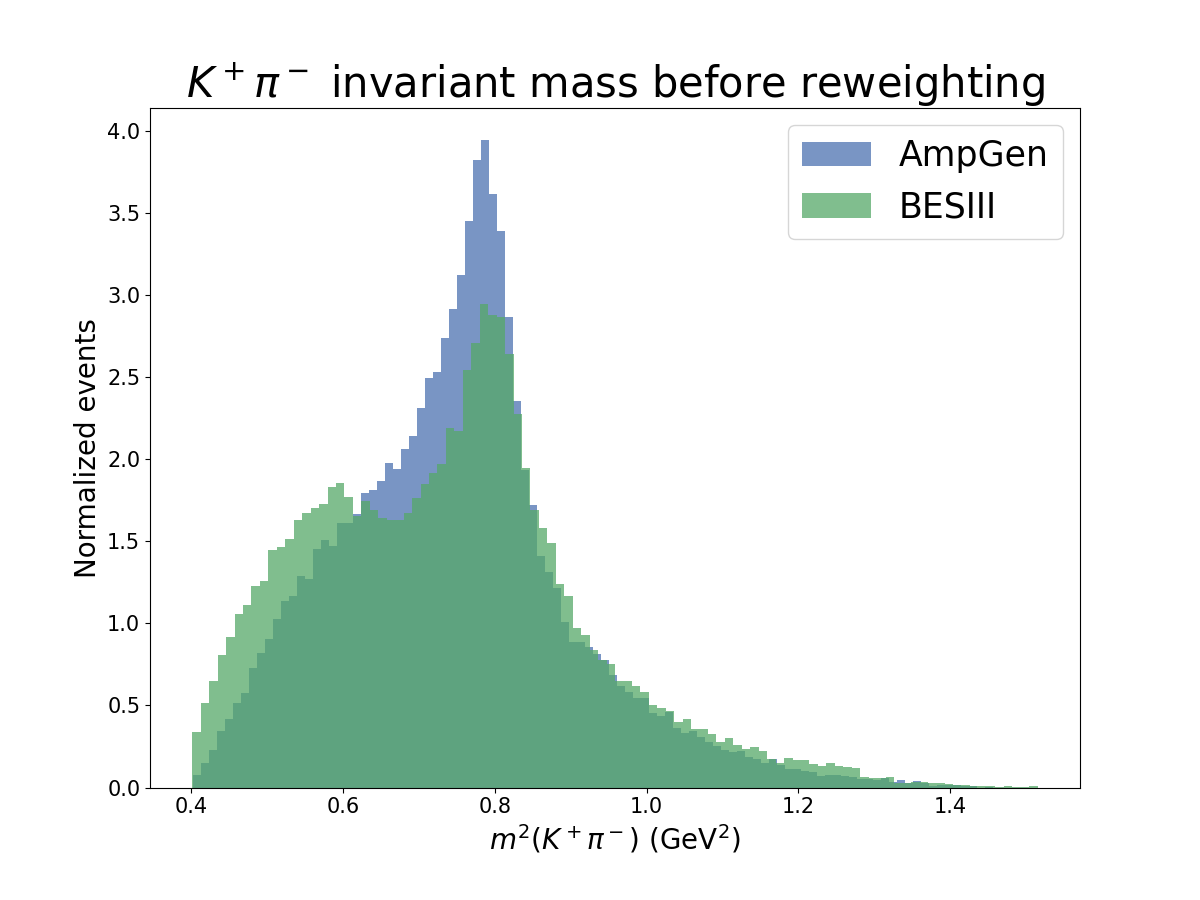
\includegraphics[width = 1.0\textwidth]{Plots/s03_BeforeReweighting.png}
      \caption{$m^2(K^+\pi^-)$}
    \end{subfigure}%
    \begin{subfigure}{0.33\textwidth}
      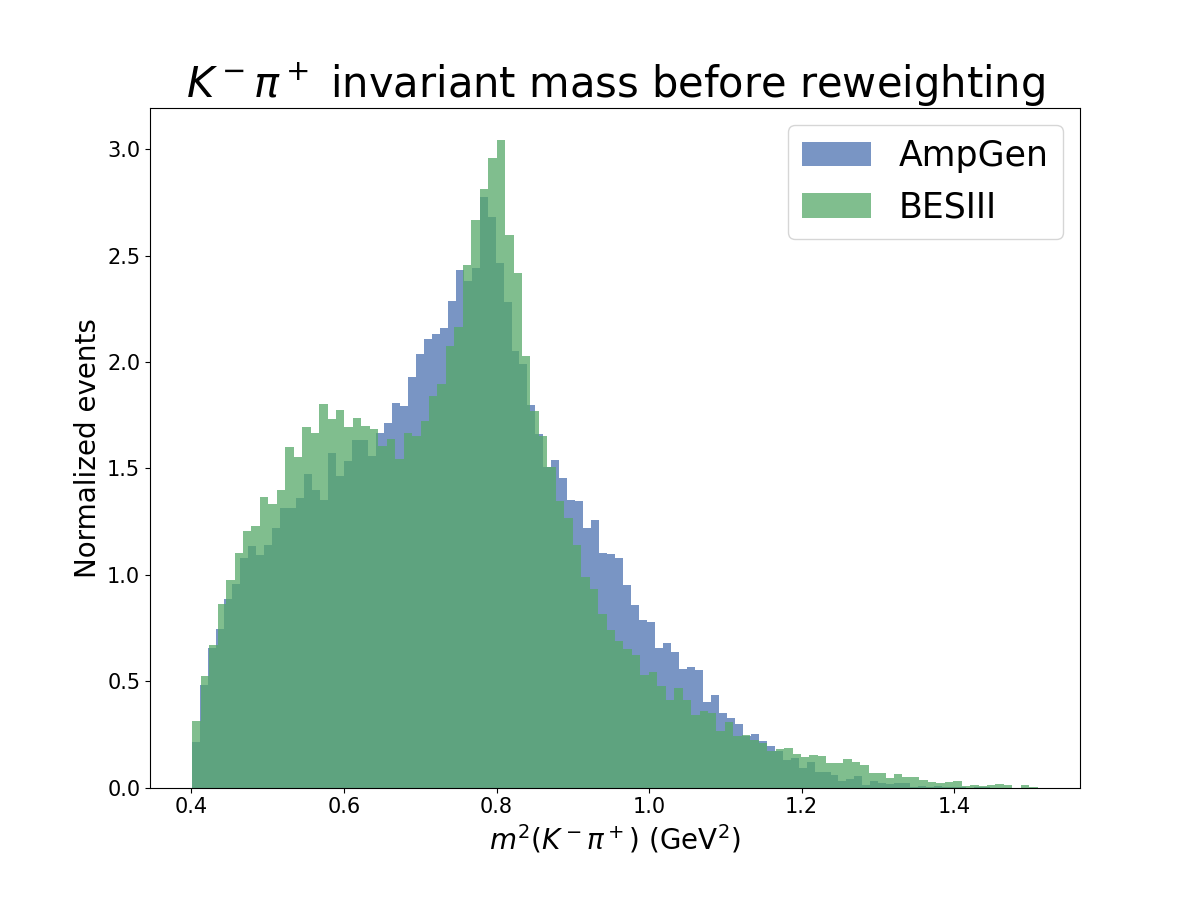
\includegraphics[width = 1.0\textwidth]{Plots/s12_BeforeReweighting.png}
      \caption{$m^2(K^-\pi^+)$}
    \end{subfigure}
    \begin{subfigure}{0.33\textwidth}
      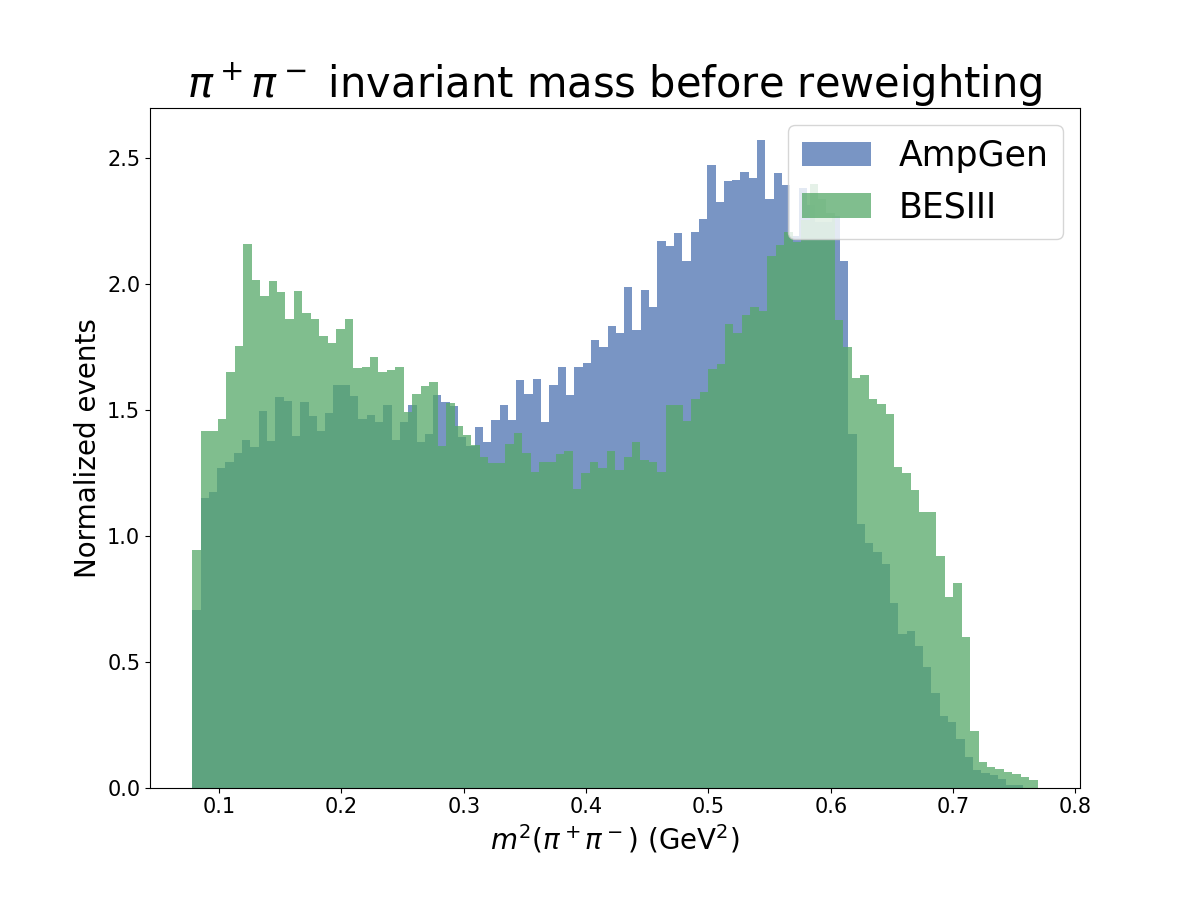
\includegraphics[width = 1.0\textwidth]{Plots/s23_BeforeReweighting.png}
      \caption{$m^2(\pi^+\pi^-)$}
    \end{subfigure}%
    \begin{subfigure}{0.33\textwidth}
      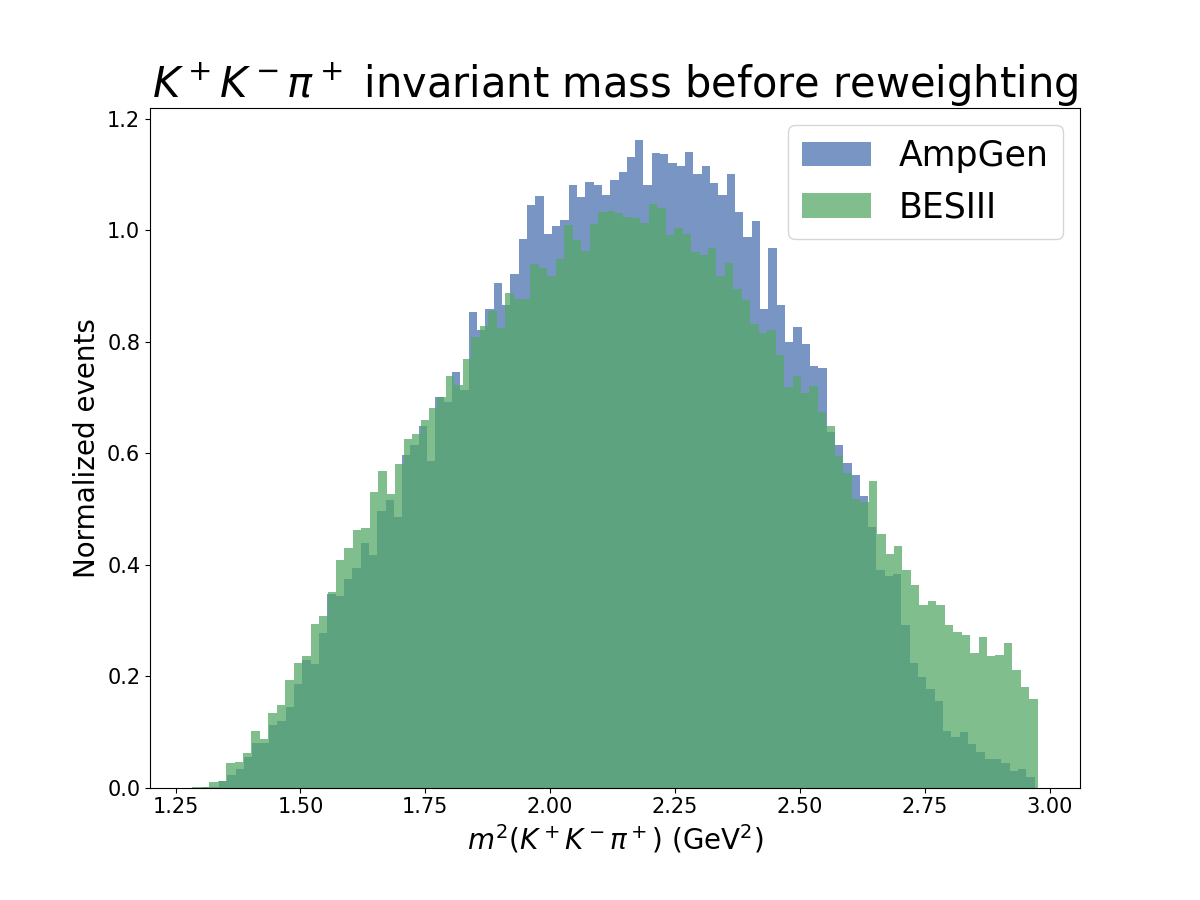
\includegraphics[width = 1.0\textwidth]{Plots/s012_BeforeReweighting.png}
      \caption{$m^2(K^+K^-\pi^+)$}
    \end{subfigure}
    \caption{Before reweighting}
  \end{figure}
\end{frame}

\begin{frame}{Naive efficiency correction}
  \begin{figure}
    \begin{subfigure}{0.33\textwidth}
      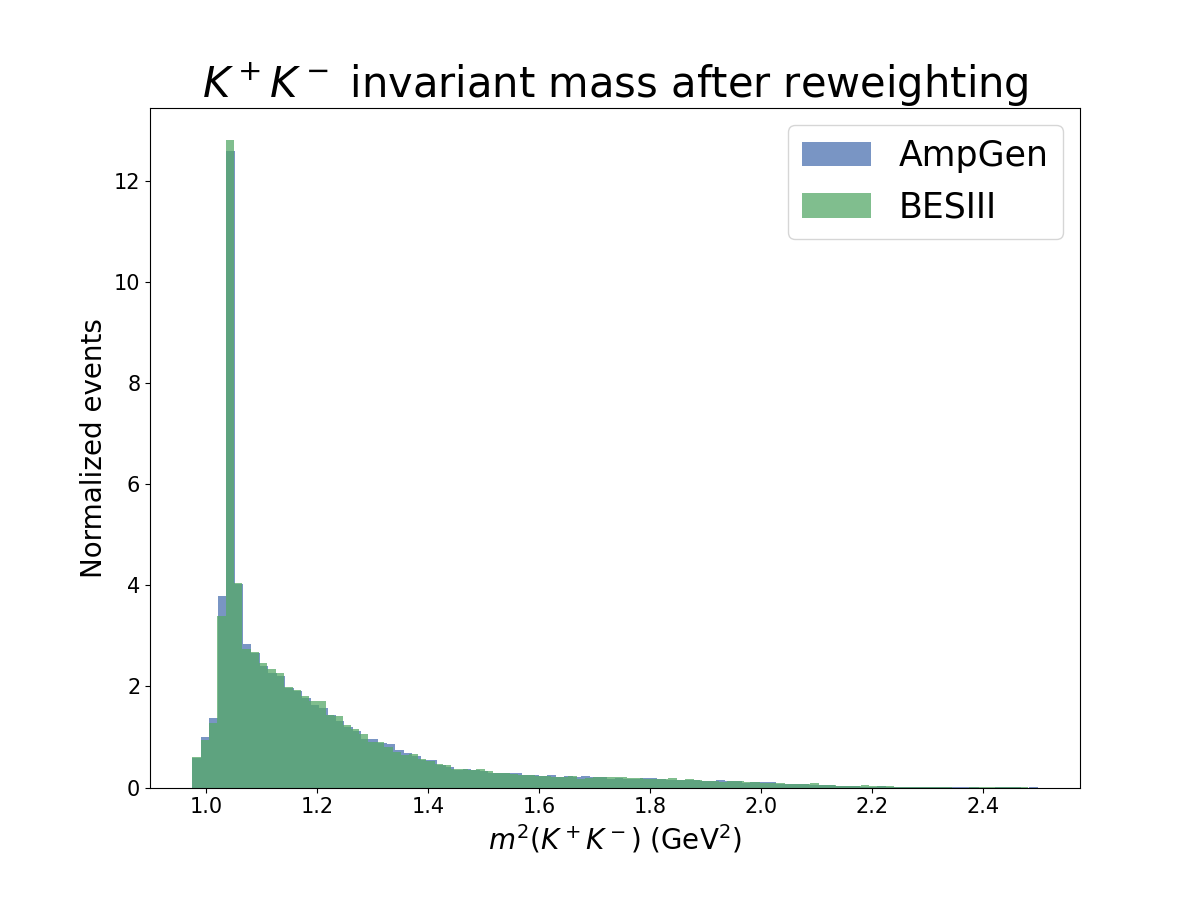
\includegraphics[width = 1.0\textwidth]{Plots/s01_AfterReweighting.png}
      \caption{$m^2(K^+K^-)$}
    \end{subfigure}%
    \begin{subfigure}{0.33\textwidth}
      \includegraphics[width = 1.0\textwidth]{Plots/s03_AfterReweighting.png}
      \caption{$m^2(K^+\pi^-)$}
    \end{subfigure}%
    \begin{subfigure}{0.33\textwidth}
      \includegraphics[width = 1.0\textwidth]{Plots/s12_AfterReweighting.png}
      \caption{$m^2(K^-\pi^+)$}
    \end{subfigure}
    \begin{subfigure}{0.33\textwidth}
      \includegraphics[width = 1.0\textwidth]{Plots/s23_AfterReweighting.png}
      \caption{$m^2(\pi^+\pi^-)$}
    \end{subfigure}%
    \begin{subfigure}{0.33\textwidth}
      \includegraphics[width = 1.0\textwidth]{Plots/s012_AfterReweighting.png}
      \caption{$m^2(K^+K^-\pi^+)$}
    \end{subfigure}
    \caption{After reweighting}
  \end{figure}
\end{frame}

\begin{frame}{Does the naive reweighting work?}
  \begin{figure}
    \begin{subfigure}{0.33\textwidth}
      \includegraphics[width = 1.0\textwidth]{Plots/s01_DataMCMismatch_BeforeReweighting.png}
      \caption{$m^2(K^+K^-)$}
    \end{subfigure}%
    \begin{subfigure}{0.33\textwidth}
      \includegraphics[width = 1.0\textwidth]{Plots/s03_DataMCMismatch_BeforeReweighting.png}
      \caption{$m^2(K^+\pi^-)$}
    \end{subfigure}%
    \begin{subfigure}{0.33\textwidth}
      \includegraphics[width = 1.0\textwidth]{Plots/s12_DataMCMismatch_BeforeReweighting.png}
      \caption{$m^2(K^-\pi^+)$}
    \end{subfigure}
    \begin{subfigure}{0.33\textwidth}
      \includegraphics[width = 1.0\textwidth]{Plots/s23_DataMCMismatch_BeforeReweighting.png}
      \caption{$m^2(\pi^+\pi^-)$}
    \end{subfigure}%
    \begin{subfigure}{0.33\textwidth}
      \includegraphics[width = 1.0\textwidth]{Plots/s012_DataMCMismatch_BeforeReweighting.png}
      \caption{$m^2(K^+K^-\pi^+)$}
    \end{subfigure}
    \caption{Single tag $D\to KK\pi\pi$ in data and MC after reweighting}
  \end{figure}
\end{frame}

\begin{frame}{Quantum correlated LHCb model}
  \begin{itemize}
    \setlength\itemsep{1.5em}
    \item{Problem with naive reweighting:}
    \begin{itemize}
    \setlength\itemsep{1.0em}
      \item{LHCb model assumes a pure $D^0\to K^+K^-\pi^+\pi^-$ decay}
      \item{\underline{No} quantum correlations}
      \item{Example: If tag is $D\to KK$, the $D\to KK\pi\pi$ decay will be CP odd!}
      \item{Quantum correlations will affect phase space distribution $\implies$ Efficiencies could change}
    \end{itemize}
    \item{Solution: Separate reweighters for CP even/odd $D\to K^+K^-\pi^+\pi^-$}
    \begin{itemize}
    \setlength\itemsep{1.0em}
      \item{CP even tags: Use efficiencies after reweighting to CP odd model}
      \item{CP odd tags: Use efficiencies after reweighting to CP even model}
      \item{$K_{S, L}\pi\pi$ tags: Do a weighted average of the two efficiencies}
    \end{itemize}
  \end{itemize}
\end{frame}

\begin{frame}{Before weighting to CP even/odd models}
  \begin{figure}
    \begin{subfigure}{0.50\textwidth}
      \includegraphics[width = 1.0\textwidth]{Plots/s23_BeforeReweighting_CPEven.png}
      \caption{CP even}
    \end{subfigure}%
    \begin{subfigure}{0.50\textwidth}
      \includegraphics[width = 1.0\textwidth]{Plots/s23_BeforeReweighting_CPOdd.png}
      \caption{CP odd}
    \end{subfigure}
    \caption{$m^2(\pi^+\pi^-)$ before reweighting}
  \end{figure}
\end{frame}

\begin{frame}{After weighting to CP even/odd models}
  \begin{figure}
    \begin{subfigure}{0.50\textwidth}
      \includegraphics[width = 1.0\textwidth]{Plots/s23_AfterReweighting_CPEven.png}
      \caption{CP even}
    \end{subfigure}%
    \begin{subfigure}{0.50\textwidth}
      \includegraphics[width = 1.0\textwidth]{Plots/s23_AfterReweighting_CPOdd.png}
      \caption{CP odd}
    \end{subfigure}
    \caption{$m^2(\pi^+\pi^-)$ after reweighting}
  \end{figure}
  \vspace{-0.4cm}
  \begin{tabular}{cccc}
    \hline
    No reweighting & Naive reweighting & CP even model & CP odd model \\
    \hline
    $18.0\%$       & $19.0\%$          & $18.1\%$      & $21.9\%$ \\
    \hline
  \end{tabular}
\end{frame}

\begin{frame}{Agreement between quantum correlated data and model}
  \begin{itemize}
    \item{Note: LHCb model knows \underline{nothing} about quantum correlations}
    \item{$D^0$/$\bar{D^0}$ amplitudes simply combined to obtain CP even/odd models}
    \item{Important question: Can the model describe quantum correlated double tag data at all? Answer: Yes!}
  \end{itemize}
  \begin{figure}
    \begin{subfigure}{0.50\textwidth}
      \includegraphics[width = 1.0\textwidth]{Plots/s23_DataModel_CPEvenTags.png}
      \caption{Double tags of $KK\pi\pi$ vs CP even}
    \end{subfigure}%
    \begin{subfigure}{0.50\textwidth}
      \includegraphics[width = 1.0\textwidth]{Plots/s23_DataModel_CPOddTags.png}
      \caption{Double tags of $KK\pi\pi$ vs CP odd}
    \end{subfigure}
    \caption{$m^2(\pi^+\pi^-)$ in double tags, compared with CP even/odd LHCb models}
  \end{figure}
\end{frame}

\section{\texorpdfstring{$F_+$}{F+} combination}

\begin{frame}{$F_+$ measurement with CP tags}
  \begin{figure}
    \centering
    \includegraphics[width=0.75\textwidth]{Plots/CPeven_fraction_combination_CPtags.png}
    \caption{$F_+$ combination of CP tags\\Fit result: $F_+ = \SI{0.703(42)}{}$, $\chi^2 = 1.4$}
  \end{figure}
\end{frame}

\begin{frame}{$F_+$ measurement with $K_{S, L}\pi\pi$ tags}
  \begin{figure}
    \centering
    \vspace{-0.2cm}
    \begin{subfigure}{0.50\textwidth}
      \includegraphics[width = 1.0\textwidth]{Plots/CPeven_fraction_combination_KSpipi.png}
      \caption{Result: $F_+ = \SI{0.872(91)}{}$, $\chi^2 = 1.3$}
    \end{subfigure}%
    \begin{subfigure}{0.50\textwidth}
      \includegraphics[width = 1.0\textwidth]{Plots/CPeven_fraction_combination_KLpipi.png}
      \caption{Result: $F_+ = \SI{0.679(103)}{}$, $\chi^2 = 0.8$}
    \end{subfigure}
    \caption{$F_+$ combination of $K_S\pi\pi$ (left) and $K_L\pi\pi$ (right)}
  \end{figure}
\end{frame}

\begin{frame}{$F_+$ combination}
  \begin{figure}
    \includegraphics[width = 0.55\textwidth]{Plots/FPlus_contours.png}
    \caption{$F_+$ combination}
  \end{figure}
  \vspace{-0.6cm}
  \begin{itemize}
    \item{Observe large anti-correlation in $K_L\pi\pi$ because $F^{K_L\pi\pi}_+\approx 0.354$}
    \begin{itemize}
      \item{Yield of $K_L\pi\pi$ is \underline{twice} as large as that of $K_S\pi\pi$}
      \item{Fractional bin yields \underline{and} total yield contains information about $F_+$}
      \item{When $K_L\pi\pi$ BF is available, combine all tags!}
    \end{itemize}
  \end{itemize}
\end{frame}

\section{Systematics}

\begin{frame}{Systematics}
  \begin{center}
    \def\arraystretch{1.2}%
    Tag-specific systematic uncertainties, in units of $10^{-2}$ \\
    \begin{tabular}{lcc}
      \hline
      Source                   & CP tags & $K_{S, L}\pi\pi$ tags \\
      \hline
      Efficiency               & $0.1$   & $0.4$ \\
      External inputs          & $0.3$   & $0.8$ \\
      Peaking backgrounds      & $0.2$   & $0.3$ \\
      $K^0_L\pi^0$ ST yield    & $2.1$   & N/A \\
      Efficiency factorisation & $0.6$   & N/A \\
      \hline
      Total                    & $2.2$   & $0.9$ \\
      \hline
    \end{tabular}
  \end{center}
  \begin{center}
    \def\arraystretch{1.2}%
    Common systematic uncertainties, in units of $10^{-2}$ \\
    \begin{tabular}{lc}
      \hline
      Source                 & Common systematic \\
      \hline
      Efficiency reweighting & $1.5$ \\
      $K^0_S$ veto           & $0.8$ \\
      \hline
    \end{tabular}
  \end{center}
\end{frame}

\section{Summary and conclusion}

\begin{frame}{Summary}
  \begin{itemize}
    \setlength\itemsep{1.0em}
    \item{First model-independent measurement of CP even fraction in $D^0\to K^+K^-\pi^+\pi^-$}
    \begin{itemize}
      \item{Analysis is now ready for review}
      \item{$F_+ = 0.730 \pm 0.040 \pm 0.017$}
      \item{Statistics dominated!}
      \item{Very consistent with model prediction: $F_+ = 0.736$}
    \end{itemize}
    \item{Valuable input to:}
    \begin{itemize}
      \item{$\gamma$ measurement with GLW method}
      \item{$D$-mixing and CPV analyses}
    \end{itemize}
    \item{Future $\psi(3770)$ data will allow us to perform a binned analysis}
  \end{itemize}
  \vspace{0.4cm}
  \begin{center}
    {\huge Thank you!}
  \end{center}
\end{frame}

\begin{frame}{Backup}
  \begin{center}
    {\huge Backup}
  \end{center}
\end{frame}

\begin{frame}{Tag modes}
  \begin{itemize}
    \setlength\itemsep{1.0em}
    \item{Flavour tags:}
    \begin{itemize}
      \item{$K\pi$, $K\pi\pi^0$, $K\pi\pi\pi$, \underline{$Ke\nu$}}
    \end{itemize}
    \item{CP even tags:}
    \begin{itemize}
      \item{$KK$, $\pi\pi$, $\pi\pi\pi^0$ (mostly CP even), $K_S\pi^0\pi^0$, $K_L\pi^0$}
    \end{itemize}
    \item{CP odd tags:}
    \begin{itemize}
      \item{$K_S\pi^0$, $K_S\eta$, $K_S\omega$, $K_S\eta^\prime_{\pi\pi\eta}$, $K_S\eta^\prime_{\rho\gamma}$}
    \end{itemize}
    \item{Self-conjugate tags:}
    \begin{itemize}
      \item{$K_S\pi\pi$, $K_L\pi\pi$}
    \end{itemize}
  \end{itemize}
  Underlined tags have not been finalized yet
\end{frame}

\begin{frame}{Double tag fits}
  \begin{figure}
    \centering
    \includegraphics[width=0.32\textwidth, clip = true, trim = {0 11cm 0 0}]{Plots/DoubleTagYield_DoubleTag_SCMB_KKpipi_vs_KSpipiPartReco_SignalBin0_TagBin1.png}
    \includegraphics[width=0.32\textwidth, clip = true, trim = {0 11cm 0 0}]{Plots/DoubleTagYield_DoubleTag_SCMB_KKpipi_vs_KSpipiPartReco_SignalBin0_TagBin2.png}
    \includegraphics[width=0.32\textwidth, clip = true, trim = {0 11cm 0 0}]{Plots/DoubleTagYield_DoubleTag_SCMB_KKpipi_vs_KSpipiPartReco_SignalBin0_TagBin3.png}
    \includegraphics[width=0.32\textwidth, clip = true, trim = {0 11cm 0 0}]{Plots/DoubleTagYield_DoubleTag_SCMB_KKpipi_vs_KSpipiPartReco_SignalBin0_TagBin4.png}
    \includegraphics[width=0.32\textwidth, clip = true, trim = {0 11cm 0 0}]{Plots/DoubleTagYield_DoubleTag_SCMB_KKpipi_vs_KSpipiPartReco_SignalBin0_TagBin5.png}
    \includegraphics[width=0.32\textwidth, clip = true, trim = {0 11cm 0 0}]{Plots/DoubleTagYield_DoubleTag_SCMB_KKpipi_vs_KSpipiPartReco_SignalBin0_TagBin6.png}
    \includegraphics[width=0.32\textwidth, clip = true, trim = {0 11cm 0 0}]{Plots/DoubleTagYield_DoubleTag_SCMB_KKpipi_vs_KSpipiPartReco_SignalBin0_TagBin7.png}
    \includegraphics[width=0.32\textwidth, clip = true, trim = {0 11cm 0 0}]{Plots/DoubleTagYield_DoubleTag_SCMB_KKpipi_vs_KSpipiPartReco_SignalBin0_TagBin8.png}
    \caption{Partially reconstructed $KK\pi\pi$ vs $K_S\pi\pi$ simultaneous fit}
  \end{figure}
\end{frame}

\begin{frame}{Double tag fits}
  \begin{figure}
    \centering
    \includegraphics[width=0.32\textwidth, clip = true, trim = {0 11cm 0 0}]{Plots/DoubleTagYield_DoubleTag_SCMB_KKpipi_vs_KLpipi_SignalBin0_TagBin1.png}
    \includegraphics[width=0.32\textwidth, clip = true, trim = {0 11cm 0 0}]{Plots/DoubleTagYield_DoubleTag_SCMB_KKpipi_vs_KLpipi_SignalBin0_TagBin2.png}
    \includegraphics[width=0.32\textwidth, clip = true, trim = {0 11cm 0 0}]{Plots/DoubleTagYield_DoubleTag_SCMB_KKpipi_vs_KLpipi_SignalBin0_TagBin3.png}
    \includegraphics[width=0.32\textwidth, clip = true, trim = {0 11cm 0 0}]{Plots/DoubleTagYield_DoubleTag_SCMB_KKpipi_vs_KLpipi_SignalBin0_TagBin4.png}
    \includegraphics[width=0.32\textwidth, clip = true, trim = {0 11cm 0 0}]{Plots/DoubleTagYield_DoubleTag_SCMB_KKpipi_vs_KLpipi_SignalBin0_TagBin5.png}
    \includegraphics[width=0.32\textwidth, clip = true, trim = {0 11cm 0 0}]{Plots/DoubleTagYield_DoubleTag_SCMB_KKpipi_vs_KLpipi_SignalBin0_TagBin6.png}
    \includegraphics[width=0.32\textwidth, clip = true, trim = {0 11cm 0 0}]{Plots/DoubleTagYield_DoubleTag_SCMB_KKpipi_vs_KLpipi_SignalBin0_TagBin7.png}
    \includegraphics[width=0.32\textwidth, clip = true, trim = {0 11cm 0 0}]{Plots/DoubleTagYield_DoubleTag_SCMB_KKpipi_vs_KLpipi_SignalBin0_TagBin8.png}
    \caption{$KK\pi\pi$ vs $K_L\pi\pi$ simultaneous fit}
  \end{figure}
\end{frame}

\begin{frame}{Peaking backgrounds}
  \begin{itemize}
    \item{Strategy for fixing peaking backgrounds:}
    \begin{enumerate}
      \item{Generate dedicated MC sample}
      \item{Obtain retention rate of peaking background}
      \item{Fit background with appropriate shape (Gaussian, Crystal Ball, ...)}
      \item{Use BFs from PDG to fix background-to-signal ratio}
    \end{enumerate}
  \end{itemize}
  \begin{figure}
    \centering
    \includegraphics[width=0.50\textwidth]{Plots/KSKKtoKKpipi_Fit.png}
    \caption{Double Gaussian fit of $K_SKK$ background in $KK\pi\pi$ single tag fit}
  \end{figure}
\end{frame}

\begin{frame}{Quantum correlation in peaking backgrounds}
  \begin{itemize}
    \item{Strategy for peaking backgrounds with different CP:}
    \begin{itemize}
      \item{Correct using $F_+^{KK\pi\pi}$ from LHCb model}
    \end{itemize}
    \item{Strategy for $K_SKK$ background in $KK\pi\pi$}
    \begin{itemize}
      \item{$F_+^{K_SKK} = \SI{0.524(18)}{}$ from \href{https://arxiv.org/abs/2007.07959}{Phys. Rev. D \textbf{102}, 052008}}
      \item{Use dedicated MC to find retention in each $K_SKK$ bin}
      \item{$K_S$ veto removes more $K_S\phi$ than $K_Sa(980)^0$ $\implies$ Calculate effective $F_+$ for $K_SKK$ to $KK\pi\pi$ background}
    \end{itemize}
  \end{itemize}
\end{frame}

\end{document}
